% **************************************************************************************************************
% A Classic Thesis Style
% An Homage to The Elements of Typographic Style
%
% Copyright (C) 2015 André Miede http://www.miede.de
%
% If you like the style then I would appreciate a postcard. My address
% can be found in the file ClassicThesis.pdf. A collection of the
% postcards I received so far is available online at
% http://postcards.miede.de
%
% License:
% This program is free software; you can redistribute it and/or modify
% it under the terms of the GNU General Public License as published by
% the Free Software Foundation; either version 2 of the License, or
% (at your option) any later version.
%
% This program is distributed in the hope that it will be useful,
% but WITHOUT ANY WARRANTY; without even the implied warranty of
% MERCHANTABILITY or FITNESS FOR A PARTICULAR PURPOSE.  See the
% GNU General Public License for more details.
%
% You should have received a copy of the GNU General Public License
% along with this program; see the file COPYING.  If not, write to
% the Free Software Foundation, Inc., 59 Temple Place - Suite 330,
% Boston, MA 02111-1307, USA.
%
% **************************************************************************************************************
\RequirePackage{fix-cm} % fix some latex issues see: http://texdoc.net/texmf-dist/doc/latex/base/fixltx2e.pdf
\documentclass[ twoside,openright,titlepage,numbers=noenddot,headinclude,%1headlines,% letterpaper a4paper
                footinclude=true,cleardoublepage=empty,abstractoff, % <--- obsolete, remove (todo)
                BCOR=5mm,paper=a4,fontsize=11pt,%11pt,a4paper,%
                ngerman,american,%
                ]{scrreprt}

%********************************************************************
% Note: Make all your adjustments in here
%*******************************************************
% ****************************************************************************************************
% classicthesis-config.tex
% formerly known as loadpackages.sty, classicthesis-ldpkg.sty, and classicthesis-preamble.sty
% Use it at the beginning of your ClassicThesis.tex, or as a LaTeX Preamble
% in your ClassicThesis.{tex,lyx} with % ****************************************************************************************************
% classicthesis-config.tex 
% formerly known as loadpackages.sty, classicthesis-ldpkg.sty, and classicthesis-preamble.sty 
% Use it at the beginning of your ClassicThesis.tex, or as a LaTeX Preamble 
% in your ClassicThesis.{tex,lyx} with % ****************************************************************************************************
% classicthesis-config.tex 
% formerly known as loadpackages.sty, classicthesis-ldpkg.sty, and classicthesis-preamble.sty 
% Use it at the beginning of your ClassicThesis.tex, or as a LaTeX Preamble 
% in your ClassicThesis.{tex,lyx} with \input{classicthesis-config}
% ****************************************************************************************************  
% If you like the classicthesis, then I would appreciate a postcard. 
% My address can be found in the file ClassicThesis.pdf. A collection 
% of the postcards I received so far is available online at 
% http://postcards.miede.de
% ****************************************************************************************************


% ****************************************************************************************************
% 0. Set the encoding of your files. UTF-8 is the only sensible encoding nowadays. If you can't read
% äöüßáéçèê∂åëæƒÏ€ then change the encoding setting in your editor, not the line below. If your editor
% does not support utf8 use another editor!
% ****************************************************************************************************
\PassOptionsToPackage{utf8}{inputenc}
	\usepackage{inputenc}

% ****************************************************************************************************
% 1. Configure classicthesis for your needs here, e.g., remove "drafting" below 
% in order to deactivate the time-stamp on the pages
% ****************************************************************************************************
\PassOptionsToPackage{eulerchapternumbers,listings,drafting,%
					 pdfspacing,%floatperchapter,%linedheaders,%
					 subfig,beramono,eulermath,parts}{classicthesis}                                        
% ********************************************************************
% Available options for classicthesis.sty 
% (see ClassicThesis.pdf for more information):
% drafting
% parts nochapters linedheaders
% eulerchapternumbers beramono eulermath pdfspacing minionprospacing
% tocaligned dottedtoc manychapters
% listings floatperchapter subfig
% ********************************************************************


% ****************************************************************************************************
% 2. Personal data and user ad-hoc commands
% ****************************************************************************************************
\newcommand{\myTitle}{A Classic Thesis Style\xspace}
\newcommand{\mySubtitle}{An Homage to The Elements of Typographic Style\xspace}
\newcommand{\myDegree}{Doktor-Ingenieur (Dr.-Ing.)\xspace}
\newcommand{\myName}{André Miede\xspace}
\newcommand{\myProf}{Put name here\xspace}
\newcommand{\myOtherProf}{Put name here\xspace}
\newcommand{\mySupervisor}{Put name here\xspace}
\newcommand{\myFaculty}{Put data here\xspace}
\newcommand{\myDepartment}{Put data here\xspace}
\newcommand{\myUni}{Put data here\xspace}
\newcommand{\myLocation}{Saarbrücken\xspace}
\newcommand{\myTime}{September 2015\xspace}
\newcommand{\myVersion}{version 4.2\xspace}

% ********************************************************************
% Setup, finetuning, and useful commands
% ********************************************************************
\newcounter{dummy} % necessary for correct hyperlinks (to index, bib, etc.)
\newlength{\abcd} % for ab..z string length calculation
\providecommand{\mLyX}{L\kern-.1667em\lower.25em\hbox{Y}\kern-.125emX\@}
\newcommand{\ie}{i.\,e.}
\newcommand{\Ie}{I.\,e.}
\newcommand{\eg}{e.\,g.}
\newcommand{\Eg}{E.\,g.} 
% ****************************************************************************************************


% ****************************************************************************************************
% 3. Loading some handy packages
% ****************************************************************************************************
% ******************************************************************** 
% Packages with options that might require adjustments
% ******************************************************************** 
%\PassOptionsToPackage{ngerman,american}{babel}   % change this to your language(s)
% Spanish languages need extra options in order to work with this template
%\PassOptionsToPackage{spanish,es-lcroman}{babel}
	\usepackage{babel}                  

\usepackage{csquotes}
\PassOptionsToPackage{%
    %backend=biber, %instead of bibtex
	backend=bibtex8,bibencoding=ascii,%
	language=auto,%
	style=numeric-comp,%
    %style=authoryear-comp, % Author 1999, 2010
    %bibstyle=authoryear,dashed=false, % dashed: substitute rep. author with ---
    sorting=nyt, % name, year, title
    maxbibnames=10, % default: 3, et al.
    %backref=true,%
    natbib=true % natbib compatibility mode (\citep and \citet still work)
}{biblatex}
    \usepackage{biblatex}

\PassOptionsToPackage{fleqn}{amsmath}       % math environments and more by the AMS 
    \usepackage{amsmath}

% ******************************************************************** 
% General useful packages
% ******************************************************************** 
\PassOptionsToPackage{T1}{fontenc} % T2A for cyrillics
    \usepackage{fontenc}     
\usepackage{textcomp} % fix warning with missing font shapes
\usepackage{scrhack} % fix warnings when using KOMA with listings package          
\usepackage{xspace} % to get the spacing after macros right  
\usepackage{mparhack} % get marginpar right
\usepackage{fixltx2e} % fixes some LaTeX stuff --> since 2015 in the LaTeX kernel (see below)
%\usepackage[latest]{latexrelease} % will be used once available in more distributions (ISSUE #107)
\PassOptionsToPackage{printonlyused,smaller}{acronym} 
    \usepackage{acronym} % nice macros for handling all acronyms in the thesis
    %\renewcommand{\bflabel}[1]{{#1}\hfill} % fix the list of acronyms --> no longer working
    %\renewcommand*{\acsfont}[1]{\textsc{#1}} 
    \renewcommand*{\aclabelfont}[1]{\acsfont{#1}}
% ****************************************************************************************************


% ****************************************************************************************************
% 4. Setup floats: tables, (sub)figures, and captions
% ****************************************************************************************************
\usepackage{tabularx} % better tables
    \setlength{\extrarowheight}{3pt} % increase table row height
\newcommand{\tableheadline}[1]{\multicolumn{1}{c}{\spacedlowsmallcaps{#1}}}
\newcommand{\myfloatalign}{\centering} % to be used with each float for alignment
\usepackage{caption}
% Thanks to cgnieder and Claus Lahiri
% http://tex.stackexchange.com/questions/69349/spacedlowsmallcaps-in-caption-label
% [REMOVED DUE TO OTHER PROBLEMS, SEE ISSUE #82]    
%\DeclareCaptionLabelFormat{smallcaps}{\bothIfFirst{#1}{~}\MakeTextLowercase{\textsc{#2}}}
%\captionsetup{font=small,labelformat=smallcaps} % format=hang,
\captionsetup{font=small} % format=hang,
\usepackage{subfig}  
% ****************************************************************************************************


% ****************************************************************************************************
% 5. Setup code listings
% ****************************************************************************************************
\usepackage{listings} 
%\lstset{emph={trueIndex,root},emphstyle=\color{BlueViolet}}%\underbar} % for special keywords
\lstset{language=[LaTeX]Tex,%C++,
    morekeywords={PassOptionsToPackage,selectlanguage},
    keywordstyle=\color{RoyalBlue},%\bfseries,
    basicstyle=\small\ttfamily,
    %identifierstyle=\color{NavyBlue},
    commentstyle=\color{Green}\ttfamily,
    stringstyle=\rmfamily,
    numbers=none,%left,%
    numberstyle=\scriptsize,%\tiny
    stepnumber=5,
    numbersep=8pt,
    showstringspaces=false,
    breaklines=true,
    %frameround=ftff,
    %frame=single,
    belowcaptionskip=.75\baselineskip
    %frame=L
} 
% ****************************************************************************************************             


% ****************************************************************************************************
% 6. PDFLaTeX, hyperreferences and citation backreferences
% ****************************************************************************************************
% ********************************************************************
% Using PDFLaTeX
% ********************************************************************
\PassOptionsToPackage{pdftex,hyperfootnotes=false,pdfpagelabels}{hyperref}
    \usepackage{hyperref}  % backref linktocpage pagebackref
\pdfcompresslevel=9
\pdfadjustspacing=1 
\PassOptionsToPackage{pdftex}{graphicx}
    \usepackage{graphicx} 
 

% ********************************************************************
% Hyperreferences
% ********************************************************************
\hypersetup{%
    %draft, % = no hyperlinking at all (useful in b/w printouts)
    colorlinks=true, linktocpage=true, pdfstartpage=3, pdfstartview=FitV,%
    % uncomment the following line if you want to have black links (e.g., for printing)
    %colorlinks=false, linktocpage=false, pdfstartpage=3, pdfstartview=FitV, pdfborder={0 0 0},%
    breaklinks=true, pdfpagemode=UseNone, pageanchor=true, pdfpagemode=UseOutlines,%
    plainpages=false, bookmarksnumbered, bookmarksopen=true, bookmarksopenlevel=1,%
    hypertexnames=true, pdfhighlight=/O,%nesting=true,%frenchlinks,%
    urlcolor=webbrown, linkcolor=RoyalBlue, citecolor=webgreen, %pagecolor=RoyalBlue,%
    %urlcolor=Black, linkcolor=Black, citecolor=Black, %pagecolor=Black,%
    pdftitle={\myTitle},%
    pdfauthor={\textcopyright\ \myName, \myUni, \myFaculty},%
    pdfsubject={},%
    pdfkeywords={},%
    pdfcreator={pdfLaTeX},%
    pdfproducer={LaTeX with hyperref and classicthesis}%
}   

% ********************************************************************
% Setup autoreferences
% ********************************************************************
% There are some issues regarding autorefnames
% http://www.ureader.de/msg/136221647.aspx
% http://www.tex.ac.uk/cgi-bin/texfaq2html?label=latexwords
% you have to redefine the makros for the 
% language you use, e.g., american, ngerman
% (as chosen when loading babel/AtBeginDocument)
% ********************************************************************
\makeatletter
\@ifpackageloaded{babel}%
    {%
       \addto\extrasamerican{%
			\renewcommand*{\figureautorefname}{Figure}%
			\renewcommand*{\tableautorefname}{Table}%
			\renewcommand*{\partautorefname}{Part}%
			\renewcommand*{\chapterautorefname}{Chapter}%
			\renewcommand*{\sectionautorefname}{Section}%
			\renewcommand*{\subsectionautorefname}{Section}%
			\renewcommand*{\subsubsectionautorefname}{Section}%     
                }%
       \addto\extrasngerman{% 
			\renewcommand*{\paragraphautorefname}{Absatz}%
			\renewcommand*{\subparagraphautorefname}{Unterabsatz}%
			\renewcommand*{\footnoteautorefname}{Fu\"snote}%
			\renewcommand*{\FancyVerbLineautorefname}{Zeile}%
			\renewcommand*{\theoremautorefname}{Theorem}%
			\renewcommand*{\appendixautorefname}{Anhang}%
			\renewcommand*{\equationautorefname}{Gleichung}%        
			\renewcommand*{\itemautorefname}{Punkt}%
                }%  
            % Fix to getting autorefs for subfigures right (thanks to Belinda Vogt for changing the definition)
            \providecommand{\subfigureautorefname}{\figureautorefname}%             
    }{\relax}
\makeatother


% ****************************************************************************************************
% 7. Last calls before the bar closes
% ****************************************************************************************************
% ********************************************************************
% Development Stuff
% ********************************************************************
\listfiles
%\PassOptionsToPackage{l2tabu,orthodox,abort}{nag}
%   \usepackage{nag}
%\PassOptionsToPackage{warning, all}{onlyamsmath}
%   \usepackage{onlyamsmath}

% ********************************************************************
% Last, but not least...
% ********************************************************************
\usepackage{classicthesis} 
% ****************************************************************************************************


% ****************************************************************************************************
% 8. Further adjustments (experimental)
% ****************************************************************************************************
% ********************************************************************
% Changing the text area
% ********************************************************************
%\linespread{1.05} % a bit more for Palatino
%\areaset[current]{312pt}{761pt} % 686 (factor 2.2) + 33 head + 42 head \the\footskip
%\setlength{\marginparwidth}{7em}%
%\setlength{\marginparsep}{2em}%

% ********************************************************************
% Using different fonts
% ********************************************************************
%\usepackage[oldstylenums]{kpfonts} % oldstyle notextcomp
%\usepackage[osf]{libertine}
%\usepackage[light,condensed,math]{iwona}
%\renewcommand{\sfdefault}{iwona}
%\usepackage{lmodern} % <-- no osf support :-(
%\usepackage{cfr-lm} % 
%\usepackage[urw-garamond]{mathdesign} <-- no osf support :-(
%\usepackage[default,osfigures]{opensans} % scale=0.95 
%\usepackage[sfdefault]{FiraSans}
% ****************************************************************************************************

% ****************************************************************************************************  
% If you like the classicthesis, then I would appreciate a postcard. 
% My address can be found in the file ClassicThesis.pdf. A collection 
% of the postcards I received so far is available online at 
% http://postcards.miede.de
% ****************************************************************************************************


% ****************************************************************************************************
% 0. Set the encoding of your files. UTF-8 is the only sensible encoding nowadays. If you can't read
% äöüßáéçèê∂åëæƒÏ€ then change the encoding setting in your editor, not the line below. If your editor
% does not support utf8 use another editor!
% ****************************************************************************************************
\PassOptionsToPackage{utf8}{inputenc}
	\usepackage{inputenc}

% ****************************************************************************************************
% 1. Configure classicthesis for your needs here, e.g., remove "drafting" below 
% in order to deactivate the time-stamp on the pages
% ****************************************************************************************************
\PassOptionsToPackage{eulerchapternumbers,listings,drafting,%
					 pdfspacing,%floatperchapter,%linedheaders,%
					 subfig,beramono,eulermath,parts}{classicthesis}                                        
% ********************************************************************
% Available options for classicthesis.sty 
% (see ClassicThesis.pdf for more information):
% drafting
% parts nochapters linedheaders
% eulerchapternumbers beramono eulermath pdfspacing minionprospacing
% tocaligned dottedtoc manychapters
% listings floatperchapter subfig
% ********************************************************************


% ****************************************************************************************************
% 2. Personal data and user ad-hoc commands
% ****************************************************************************************************
\newcommand{\myTitle}{A Classic Thesis Style\xspace}
\newcommand{\mySubtitle}{An Homage to The Elements of Typographic Style\xspace}
\newcommand{\myDegree}{Doktor-Ingenieur (Dr.-Ing.)\xspace}
\newcommand{\myName}{André Miede\xspace}
\newcommand{\myProf}{Put name here\xspace}
\newcommand{\myOtherProf}{Put name here\xspace}
\newcommand{\mySupervisor}{Put name here\xspace}
\newcommand{\myFaculty}{Put data here\xspace}
\newcommand{\myDepartment}{Put data here\xspace}
\newcommand{\myUni}{Put data here\xspace}
\newcommand{\myLocation}{Saarbrücken\xspace}
\newcommand{\myTime}{September 2015\xspace}
\newcommand{\myVersion}{version 4.2\xspace}

% ********************************************************************
% Setup, finetuning, and useful commands
% ********************************************************************
\newcounter{dummy} % necessary for correct hyperlinks (to index, bib, etc.)
\newlength{\abcd} % for ab..z string length calculation
\providecommand{\mLyX}{L\kern-.1667em\lower.25em\hbox{Y}\kern-.125emX\@}
\newcommand{\ie}{i.\,e.}
\newcommand{\Ie}{I.\,e.}
\newcommand{\eg}{e.\,g.}
\newcommand{\Eg}{E.\,g.} 
% ****************************************************************************************************


% ****************************************************************************************************
% 3. Loading some handy packages
% ****************************************************************************************************
% ******************************************************************** 
% Packages with options that might require adjustments
% ******************************************************************** 
%\PassOptionsToPackage{ngerman,american}{babel}   % change this to your language(s)
% Spanish languages need extra options in order to work with this template
%\PassOptionsToPackage{spanish,es-lcroman}{babel}
	\usepackage{babel}                  

\usepackage{csquotes}
\PassOptionsToPackage{%
    %backend=biber, %instead of bibtex
	backend=bibtex8,bibencoding=ascii,%
	language=auto,%
	style=numeric-comp,%
    %style=authoryear-comp, % Author 1999, 2010
    %bibstyle=authoryear,dashed=false, % dashed: substitute rep. author with ---
    sorting=nyt, % name, year, title
    maxbibnames=10, % default: 3, et al.
    %backref=true,%
    natbib=true % natbib compatibility mode (\citep and \citet still work)
}{biblatex}
    \usepackage{biblatex}

\PassOptionsToPackage{fleqn}{amsmath}       % math environments and more by the AMS 
    \usepackage{amsmath}

% ******************************************************************** 
% General useful packages
% ******************************************************************** 
\PassOptionsToPackage{T1}{fontenc} % T2A for cyrillics
    \usepackage{fontenc}     
\usepackage{textcomp} % fix warning with missing font shapes
\usepackage{scrhack} % fix warnings when using KOMA with listings package          
\usepackage{xspace} % to get the spacing after macros right  
\usepackage{mparhack} % get marginpar right
\usepackage{fixltx2e} % fixes some LaTeX stuff --> since 2015 in the LaTeX kernel (see below)
%\usepackage[latest]{latexrelease} % will be used once available in more distributions (ISSUE #107)
\PassOptionsToPackage{printonlyused,smaller}{acronym} 
    \usepackage{acronym} % nice macros for handling all acronyms in the thesis
    %\renewcommand{\bflabel}[1]{{#1}\hfill} % fix the list of acronyms --> no longer working
    %\renewcommand*{\acsfont}[1]{\textsc{#1}} 
    \renewcommand*{\aclabelfont}[1]{\acsfont{#1}}
% ****************************************************************************************************


% ****************************************************************************************************
% 4. Setup floats: tables, (sub)figures, and captions
% ****************************************************************************************************
\usepackage{tabularx} % better tables
    \setlength{\extrarowheight}{3pt} % increase table row height
\newcommand{\tableheadline}[1]{\multicolumn{1}{c}{\spacedlowsmallcaps{#1}}}
\newcommand{\myfloatalign}{\centering} % to be used with each float for alignment
\usepackage{caption}
% Thanks to cgnieder and Claus Lahiri
% http://tex.stackexchange.com/questions/69349/spacedlowsmallcaps-in-caption-label
% [REMOVED DUE TO OTHER PROBLEMS, SEE ISSUE #82]    
%\DeclareCaptionLabelFormat{smallcaps}{\bothIfFirst{#1}{~}\MakeTextLowercase{\textsc{#2}}}
%\captionsetup{font=small,labelformat=smallcaps} % format=hang,
\captionsetup{font=small} % format=hang,
\usepackage{subfig}  
% ****************************************************************************************************


% ****************************************************************************************************
% 5. Setup code listings
% ****************************************************************************************************
\usepackage{listings} 
%\lstset{emph={trueIndex,root},emphstyle=\color{BlueViolet}}%\underbar} % for special keywords
\lstset{language=[LaTeX]Tex,%C++,
    morekeywords={PassOptionsToPackage,selectlanguage},
    keywordstyle=\color{RoyalBlue},%\bfseries,
    basicstyle=\small\ttfamily,
    %identifierstyle=\color{NavyBlue},
    commentstyle=\color{Green}\ttfamily,
    stringstyle=\rmfamily,
    numbers=none,%left,%
    numberstyle=\scriptsize,%\tiny
    stepnumber=5,
    numbersep=8pt,
    showstringspaces=false,
    breaklines=true,
    %frameround=ftff,
    %frame=single,
    belowcaptionskip=.75\baselineskip
    %frame=L
} 
% ****************************************************************************************************             


% ****************************************************************************************************
% 6. PDFLaTeX, hyperreferences and citation backreferences
% ****************************************************************************************************
% ********************************************************************
% Using PDFLaTeX
% ********************************************************************
\PassOptionsToPackage{pdftex,hyperfootnotes=false,pdfpagelabels}{hyperref}
    \usepackage{hyperref}  % backref linktocpage pagebackref
\pdfcompresslevel=9
\pdfadjustspacing=1 
\PassOptionsToPackage{pdftex}{graphicx}
    \usepackage{graphicx} 
 

% ********************************************************************
% Hyperreferences
% ********************************************************************
\hypersetup{%
    %draft, % = no hyperlinking at all (useful in b/w printouts)
    colorlinks=true, linktocpage=true, pdfstartpage=3, pdfstartview=FitV,%
    % uncomment the following line if you want to have black links (e.g., for printing)
    %colorlinks=false, linktocpage=false, pdfstartpage=3, pdfstartview=FitV, pdfborder={0 0 0},%
    breaklinks=true, pdfpagemode=UseNone, pageanchor=true, pdfpagemode=UseOutlines,%
    plainpages=false, bookmarksnumbered, bookmarksopen=true, bookmarksopenlevel=1,%
    hypertexnames=true, pdfhighlight=/O,%nesting=true,%frenchlinks,%
    urlcolor=webbrown, linkcolor=RoyalBlue, citecolor=webgreen, %pagecolor=RoyalBlue,%
    %urlcolor=Black, linkcolor=Black, citecolor=Black, %pagecolor=Black,%
    pdftitle={\myTitle},%
    pdfauthor={\textcopyright\ \myName, \myUni, \myFaculty},%
    pdfsubject={},%
    pdfkeywords={},%
    pdfcreator={pdfLaTeX},%
    pdfproducer={LaTeX with hyperref and classicthesis}%
}   

% ********************************************************************
% Setup autoreferences
% ********************************************************************
% There are some issues regarding autorefnames
% http://www.ureader.de/msg/136221647.aspx
% http://www.tex.ac.uk/cgi-bin/texfaq2html?label=latexwords
% you have to redefine the makros for the 
% language you use, e.g., american, ngerman
% (as chosen when loading babel/AtBeginDocument)
% ********************************************************************
\makeatletter
\@ifpackageloaded{babel}%
    {%
       \addto\extrasamerican{%
			\renewcommand*{\figureautorefname}{Figure}%
			\renewcommand*{\tableautorefname}{Table}%
			\renewcommand*{\partautorefname}{Part}%
			\renewcommand*{\chapterautorefname}{Chapter}%
			\renewcommand*{\sectionautorefname}{Section}%
			\renewcommand*{\subsectionautorefname}{Section}%
			\renewcommand*{\subsubsectionautorefname}{Section}%     
                }%
       \addto\extrasngerman{% 
			\renewcommand*{\paragraphautorefname}{Absatz}%
			\renewcommand*{\subparagraphautorefname}{Unterabsatz}%
			\renewcommand*{\footnoteautorefname}{Fu\"snote}%
			\renewcommand*{\FancyVerbLineautorefname}{Zeile}%
			\renewcommand*{\theoremautorefname}{Theorem}%
			\renewcommand*{\appendixautorefname}{Anhang}%
			\renewcommand*{\equationautorefname}{Gleichung}%        
			\renewcommand*{\itemautorefname}{Punkt}%
                }%  
            % Fix to getting autorefs for subfigures right (thanks to Belinda Vogt for changing the definition)
            \providecommand{\subfigureautorefname}{\figureautorefname}%             
    }{\relax}
\makeatother


% ****************************************************************************************************
% 7. Last calls before the bar closes
% ****************************************************************************************************
% ********************************************************************
% Development Stuff
% ********************************************************************
\listfiles
%\PassOptionsToPackage{l2tabu,orthodox,abort}{nag}
%   \usepackage{nag}
%\PassOptionsToPackage{warning, all}{onlyamsmath}
%   \usepackage{onlyamsmath}

% ********************************************************************
% Last, but not least...
% ********************************************************************
\usepackage{classicthesis} 
% ****************************************************************************************************


% ****************************************************************************************************
% 8. Further adjustments (experimental)
% ****************************************************************************************************
% ********************************************************************
% Changing the text area
% ********************************************************************
%\linespread{1.05} % a bit more for Palatino
%\areaset[current]{312pt}{761pt} % 686 (factor 2.2) + 33 head + 42 head \the\footskip
%\setlength{\marginparwidth}{7em}%
%\setlength{\marginparsep}{2em}%

% ********************************************************************
% Using different fonts
% ********************************************************************
%\usepackage[oldstylenums]{kpfonts} % oldstyle notextcomp
%\usepackage[osf]{libertine}
%\usepackage[light,condensed,math]{iwona}
%\renewcommand{\sfdefault}{iwona}
%\usepackage{lmodern} % <-- no osf support :-(
%\usepackage{cfr-lm} % 
%\usepackage[urw-garamond]{mathdesign} <-- no osf support :-(
%\usepackage[default,osfigures]{opensans} % scale=0.95 
%\usepackage[sfdefault]{FiraSans}
% ****************************************************************************************************

% ****************************************************************************************************
% If you like the classicthesis, then I would appreciate a postcard.
% My address can be found in the file ClassicThesis.pdf. A collection
% of the postcards I received so far is available online at
% http://postcards.miede.de
% ****************************************************************************************************


% ****************************************************************************************************
% 0. Set the encoding of your files. UTF-8 is the only sensible encoding nowadays. If you can't read
% äöüßáéçèê∂åëæƒÏ€ then change the encoding setting in your editor, not the line below. If your editor
% does not support utf8 use another editor!
% ****************************************************************************************************
\PassOptionsToPackage{utf8}{inputenc}
	\usepackage{inputenc}

% ****************************************************************************************************
% 1. Configure classicthesis for your needs here, e.g., remove "drafting" below
% in order to deactivate the time-stamp on the pages
% ****************************************************************************************************
\PassOptionsToPackage{eulerchapternumbers,listings,%drafting,%
					 pdfspacing,floatperchapter,linedheaders,%
					 subfig,beramono,eulermath,parts,dottedtoc}{classicthesis}
% ********************************************************************
% Available options for classicthesis.sty
% (see ClassicThesis.pdf for more information):
% drafting
% parts nochapters linedheaders
% eulerchapternumbers beramono eulermath pdfspacing minionprospacing
% tocaligned dottedtoc manychapters
% listings floatperchapter subfig
% ********************************************************************


% ****************************************************************************************************
% 2. Personal data and user ad-hoc commands
% ****************************************************************************************************
\newcommand{\myTitle}{Simulation und Implementierung energieeffizienter Funkkommunikation für intelligente Logistiklager\xspace}
%\newcommand{\mySubtitle}{An Homage to The Elements of Typographic Style\xspace}
\newcommand{\myDegree}{cand.\,M.Sc.\xspace}
\newcommand{\myDocType}{Masterarbeit\xspace}
\newcommand{\myName}{Jens Drenhaus\xspace}
\newcommand{\myForename}{Jens\xspace}
\newcommand{\mySurname}{Drenhaus\xspace}
\newcommand{\myMatNr}{151278\xspace}
\newcommand{\myProf}{Prof.~Dr.-Ing. Christian Wietfeld\xspace}
%\newcommand{\myOtherProf}{Put name here\xspace}
\newcommand{\mySupervisor}{Robert Falkenberg, M.Sc.\xspace}
\newcommand{\myFaculty}{Fakultät für Elektrotechnik und Informationstechnik\xspace}
\newcommand{\myDepartment}{Lehrstuhl für Kommunikationsnetze\xspace}
\newcommand{\myUni}{Technische Universität Dortmund\xspace}
\newcommand{\myLocation}{Dortmund\xspace}
\newcommand{\myDay}{30.\xspace}
\newcommand{\myMonth}{Juli\xspace}
\newcommand{\myYear}{2017\xspace}
\newcommand{\myTime}{\myMonth\,\myYear\xspace}
\newcommand{\myDate}{\myDay\,\myMonth\,\myYear\xspace}
\newcommand{\myVersion}{Version 0.0\xspace}

% ********************************************************************
% Setup, finetuning, and useful commands
% ********************************************************************
\newcounter{dummy} % necessary for correct hyperlinks (to index, bib, etc.)
\newlength{\abcd} % for ab..z string length calculation
\providecommand{\mLyX}{L\kern-.1667em\lower.25em\hbox{Y}\kern-.125emX\@}
\newcommand{\ie}{i.\,e.}
\newcommand{\Ie}{I.\,e.}
\newcommand{\eg}{e.\,g.}
\newcommand{\Eg}{E.\,g.}
\newcommand{\zB}{z.\,B.\xspace}
\newcommand{\bzw}{bzw.\xspace}
% Deutsche Anführungsstriche
\newcommand{\gqq}[1]{\glqq{}#1\grqq{}}
\newcommand{\gq}[1]{\glq{}#1\grq{}}
% ****************************************************************************************************


% ****************************************************************************************************
% 3. Loading some handy packages
% ****************************************************************************************************
% ********************************************************************
% Packages with options that might require adjustments
% ********************************************************************
\PassOptionsToPackage{ngerman,english}{babel}   % change this to your language(s)
% Spanish languages need extra options in order to work with this template
%\PassOptionsToPackage{spanish,es-lcroman}{babel}
	\usepackage{babel}

\usepackage{csquotes}
\PassOptionsToPackage{%
    %backend=biber, %instead of bibtex
	backend=bibtex8,bibencoding=ascii,%
	language=auto,%
	style=numeric-comp,%
    %style=authoryear-comp, % Author 1999, 2010
    %bibstyle=authoryear,dashed=false, % dashed: substitute rep. author with ---
    %sorting=nyt, % name, year, title
    sorting=none, % by appearence
    maxbibnames=10, % default: 3, et al.
    %backref=true,%
    natbib=true % natbib compatibility mode (\citep and \citet still work)
}{biblatex}
    \usepackage{biblatex}

\PassOptionsToPackage{fleqn}{amsmath}       % math environments and more by the AMS
    \usepackage{amsmath}

% ********************************************************************
% General useful packages
% ********************************************************************
\PassOptionsToPackage{T1}{fontenc} % T2A for cyrillics
    \usepackage{fontenc}
\usepackage{textcomp} % fix warning with missing font shapes
\usepackage{scrhack} % fix warnings when using KOMA with listings package
\usepackage{xspace} % to get the spacing after macros right
\usepackage{mparhack} % get marginpar right
\usepackage{fixltx2e} % fixes some LaTeX stuff --> since 2015 in the LaTeX kernel (see below)
%\usepackage[latest]{latexrelease} % will be used once available in more distributions (ISSUE #107)
%\PassOptionsToPackage{printonlyused,smaller}{acronym}
    %\usepackage{acronym} % nice macros for handling all acronyms in the thesis
    %\renewcommand{\bflabel}[1]{{#1}\hfill} % fix the list of acronyms --> no longer working
    %\renewcommand*{\acsfont}[1]{\textsc{#1}}
    %\renewcommand*{\aclabelfont}[1]{\acsfont{#1}}

%\usepackage{todonotes}  
\usepackage{pifont}  
\usepackage{longtable}

% ****************************************************************************************************


% ****************************************************************************************************
% 4. Setup floats: tables, (sub)figures, and captions
% ****************************************************************************************************
\usepackage{tabularx} % better tables
    \setlength{\extrarowheight}{3pt} % increase table row height
\newcommand{\tableheadline}[1]{\multicolumn{1}{c}{\spacedlowsmallcaps{#1}}}
\newcommand{\myfloatalign}{\centering} % to be used with each float for alignment
\usepackage{caption}
% Thanks to cgnieder and Claus Lahiri
% http://tex.stackexchange.com/questions/69349/spacedlowsmallcaps-in-caption-label
% [REMOVED DUE TO OTHER PROBLEMS, SEE ISSUE #82]
%\DeclareCaptionLabelFormat{smallcaps}{\bothIfFirst{#1}{~}\MakeTextLowercase{\textsc{#2}}}
%\captionsetup{font=small,labelformat=smallcaps} % format=hang,
\captionsetup{font=small} % format=hang,
\usepackage{subfig}
% ****************************************************************************************************


% ****************************************************************************************************
% 5. Setup code listings
% ****************************************************************************************************
\usepackage{listings}
%\lstset{emph={trueIndex,root},emphstyle=\color{BlueViolet}}%\underbar} % for special keywords
\lstset{language=[LaTeX]Tex,%C++,
    morekeywords={PassOptionsToPackage,selectlanguage},
    keywordstyle=\color{RoyalBlue},%\bfseries,
    basicstyle=\small\ttfamily,
    %identifierstyle=\color{NavyBlue},
    commentstyle=\color{Green}\ttfamily,
    stringstyle=\rmfamily,
    numbers=none,%left,%
    numberstyle=\scriptsize,%\tiny
    stepnumber=5,
    numbersep=8pt,
    showstringspaces=false,
    breaklines=true,
    %frameround=ftff,
    %frame=single,
    belowcaptionskip=.75\baselineskip
    %frame=L
}
\renewcommand{\lstlistingname}{Quelltext}

% ****************************************************************************************************


% ****************************************************************************************************
% 6. PDFLaTeX, hyperreferences and citation backreferences
% ****************************************************************************************************
% ********************************************************************
% Using PDFLaTeX
% ********************************************************************
\PassOptionsToPackage{pdftex,hyperfootnotes=false,pdfpagelabels}{hyperref}
    \usepackage{hyperref}  % backref linktocpage pagebackref
\pdfcompresslevel=9
\pdfadjustspacing=1
\PassOptionsToPackage{pdftex}{graphicx}
    \usepackage{graphicx}


% ********************************************************************
% Hyperreferences
% ********************************************************************
\hypersetup{%
    %draft, % = no hyperlinking at all (useful in b/w printouts)
    colorlinks=true, linktocpage=true, pdfstartpage=1, pdfstartview=FitV,%
    % uncomment the following line if you want to have black links (e.g., for printing)
    %colorlinks=false, linktocpage=false, pdfstartpage=3, pdfstartview=FitV, pdfborder={0 0 0},%
    breaklinks=true, pdfpagemode=UseNone, pageanchor=true, pdfpagemode=UseOutlines,%
    plainpages=false, bookmarksnumbered, bookmarksopen=true, bookmarksopenlevel=1,%
    hypertexnames=true, pdfhighlight=/O,%nesting=true,%frenchlinks,%
    urlcolor=webbrown, linkcolor=RoyalBlue, citecolor=webgreen, %pagecolor=RoyalBlue,%
    %urlcolor=Black, linkcolor=Black, citecolor=Black, %pagecolor=Black,%
    pdftitle={\myTitle},%
    pdfauthor={\textcopyright\ \myName, \myUni, \myFaculty},%
    pdfsubject={},%
    pdfkeywords={},%
    pdfcreator={pdfLaTeX},%
    pdfproducer={LaTeX with hyperref and classicthesis}%
}

% ********************************************************************
% Setup autoreferences
% ********************************************************************
% There are some issues regarding autorefnames
% http://www.ureader.de/msg/136221647.aspx
% http://www.tex.ac.uk/cgi-bin/texfaq2html?label=latexwords
% you have to redefine the makros for the
% language you use, e.g., american, ngerman
% (as chosen when loading babel/AtBeginDocument)
% ********************************************************************
\makeatletter
\@ifpackageloaded{babel}%
    {%
       \addto\extrasamerican{%
			\renewcommand*{\figureautorefname}{Figure}%
			\renewcommand*{\tableautorefname}{Table}%
			\renewcommand*{\partautorefname}{Part}%
			\renewcommand*{\chapterautorefname}{Chapter}%
			\renewcommand*{\sectionautorefname}{Section}%
			\renewcommand*{\subsectionautorefname}{Section}%
			\renewcommand*{\subsubsectionautorefname}{Section}%
                }%
       \addto\extrasngerman{%
			\renewcommand*{\paragraphautorefname}{Absatz}%
			\renewcommand*{\subparagraphautorefname}{Unterabsatz}%
			\renewcommand*{\footnoteautorefname}{Fu\"snote}%
			\renewcommand*{\FancyVerbLineautorefname}{Zeile}%
			\renewcommand*{\theoremautorefname}{Theorem}%
			\renewcommand*{\appendixautorefname}{Anhang}%
			\renewcommand*{\equationautorefname}{Gleichung}%
			\renewcommand*{\itemautorefname}{Punkt}%
                }%
            % Fix to getting autorefs for subfigures right (thanks to Belinda Vogt for changing the definition)
            \providecommand{\subfigureautorefname}{\figureautorefname}%
    }{\relax}
\makeatother

% ********************************************************************
% Glossary
% ********************************************************************
\usepackage[style=long,nolist,nogroupskip,nonumberlist,xindy,acronyms,shortcuts]{glossaries} 
\GlsSetQuote{+}
\makeglossaries
\loadglsentries{Glossaries}
\glsunsetall % use no long on first use




% ****************************************************************************************************
% 7. Last calls before the bar closes
% ****************************************************************************************************
% ********************************************************************
% Development Stuff
% ********************************************************************
\listfiles
%\PassOptionsToPackage{l2tabu,orthodox,abort}{nag}
%   \usepackage{nag}
%\PassOptionsToPackage{warning, all}{onlyamsmath}
%   \usepackage{onlyamsmath}

% ********************************************************************
% Last, but not least...
% ********************************************************************
\usepackage{classicthesis}
% ****************************************************************************************************


% ****************************************************************************************************
% 8. Further adjustments (experimental)
% ****************************************************************************************************
% ********************************************************************
% Changing the text area
% ********************************************************************
%\linespread{1.05} % a bit more for Palatino
%\areaset[current]{312pt}{761pt} % 686 (factor 2.2) + 33 head + 42 head \the\footskip
%\setlength{\marginparwidth}{7em}%
%\setlength{\marginparsep}{2em}%

% ********************************************************************
% Using different fonts
% ********************************************************************
%\usepackage[oldstylenums]{kpfonts} % oldstyle notextcomp
%\usepackage[osf]{libertine}
%\usepackage[light,condensed,math]{iwona}
%\renewcommand{\sfdefault}{iwona}
%\usepackage{lmodern} % <-- no osf support :-(
%\usepackage{cfr-lm} %
%\usepackage[urw-garamond]{mathdesign} <-- no osf support :-(
%\usepackage[default,osfigures]{opensans} % scale=0.95
%\usepackage[sfdefault]{FiraSans}
% ****************************************************************************************************

%%************************************************
%Abkürzungen
%************************************************

\newcommand{\gr}[1]{\textbf{#1}}
\newcommand{\eng}[1]{\emph{#1}}
%Glossar Verweispfeil mit Text
\newcommand{\gloref}[1]{\glslink{#1}{\ding{43}\,Glossar} \glsadd{#1}}


\newacronym[description={Cyber-physisches System, engl. \eng{\gr{C}yber-\gr{P}hysical \gr{S}ystem}},%
	longplural={Cyber-physische Systeme, engl. \eng{\gr{C}yber-\gr{P}hysical \gr{S}ystems}}]%
	{cps}%
	{CPS}%
	{cyber-physisches System, engl. \eng{\gr{C}yber-\gr{P}hysical \gr{S}ystem}}%
	
\newacronym[description={Vielfachzugriff mit Trägerprüfung und Kollisionserkennung, engl. \eng{\gr{C}arrier-\gr{S}ense \gr{M}ultiple \gr{A}ccess / \gr{C}ollision \gr{A}voidance}}]%
	{csma}%
	{CSMA-CA}%
	{\eng{\gr{C}arrier \gr{S}ense \gr{M}ultiple \gr{A}ccess / \gr{C}ollision \gr{A}voidance}}%
	
\newacronym[description={Drahtloses Sensornetzwerk, engl. \eng{\gr{W}ireless \gr{S}ensor \gr{N}etwork}}]%
	{wsn}%
	{WSN}%
	{drahtloses Sensornetzwerk, engl. \eng{\gr{W}ireless \gr{S}ensor \gr{N}etwork}}%
	
\newacronym[description={Zugangspunkt, engl. \eng{\gr{A}ccess \gr{P}oint}}]%
	{ap}%
	{AP}%
	{\eng{\gr{A}ccess \gr{P}oint}}%
	
\newacronym[description={Medienzugriffssteuerung, engl. \eng{\gr{M}edia \gr{A}ccess \gr{C}ontrol}}]%
	{mac}%
	{MAC}%
	{Medienzugriffssteuerung, engl. \eng{\gr{M}edia \gr{A}ccess \gr{C}ontrol}}%
	
\newacronym[description={Engl. \eng{\gr{L}ogical \gr{L}ink \gr{C}ontrol}}]%
	{llc}%
	{LLC}%
	{\eng{\gr{L}ogical \gr{L}ink \gr{C}ontrol}}%
	
\newacronym[description={Engl. \eng{\gr{E}uropean \gr{T}elecommunications \gr{S}tandards \gr{I}nstitute}}]%
	{etsi}%
	{ETSI}%
	{\eng{\gr{E}uropean \gr{T}elecommunications \gr{S}tandards \gr{I}nstitute}}%
	
\newacronym[description={Auf Deutsch etwa \gqq{erst horchen, dann sprechen}, engl. \eng{\gr{L}isten \gr{B}efore \gr{T}alk}}]%
	{lbt}%
	{LBT}%
	{\eng{\gr{L}isten \gr{B}efore \gr{T}alk}}%
	
\newacronym[description={Engl. \eng{\gr{I}nstitute of \gr{E}lectrical and \gr{E}lectronics \gr{E}ngineers}}]%
	{ieee}%
	{IEEE}%
	{\eng{\gr{I}nstitute of \gr{E}lectrical and \gr{E}lectronics \gr{E}ngineers}}%

\newacronym[description={Kurzstreckenfunkgerät, engl. \eng{\gr{S}hort \gr{R}ange \gr{D}evice}}]%
	{srd}%
	{SRD}%
	{\eng{\gr{S}hort \gr{R}ange \gr{D}evice}}%

\newacronym[description={Offene Systemvernetzung, engl. \eng{\gr{O}pen \gr{S}ystems \gr{I}nterconnection}}]%
	{osi}%
	{OSI}%
	{\eng{\gr{O}pen \gr{S}ystems \gr{I}nterconnection}}%
	
\newacronym[description={Engl. \eng{\gr{I}nternational \gr{O}rganization for \gr{S}tandardization}}]%
	{iso}%
	{ISO}%
	{\eng{\gr{I}nternational \gr{O}rganization for \gr{S}tandardization}}%
	
\newacronym[description={Identifizierung durch elektromagnetische Wellen, engl. \eng{\gr{R}adio-\gr{F}requency \gr{I}dentification}}]%
	{rfid}%
	{RFID}%
	{Identifizierung durch elektromagnetischer Wellen, engl. \eng{\gr{R}adio-\gr{F}requency \gr{I}dentification}}%
	
\newacronym[description={Globale Handelsgut Indentifikationsnummer, engl.  \eng{\gr{G}lobal \gr{T}rade \gr{I}tem \gr{N}umber}}]%
	{gtin}%
	{GTIN}%
	{globale Handelsgut Indentifikationsnummer, engl. \eng{\gr{G}lobal \gr{T}rade \gr{I}tem \gr{N}umber}}%

\newacronym[description={Elektronischer Produkt Code, engl. \eng{\gr{E}lectronic \gr{P}roduct \gr{C}ode}}]%
	{epc}%
	{EPC}%
	{\eng{\gr{E}lectronic \gr{P}roduct \gr{C}ode}}%
	
\newacronym[description={Engl. \eng{\gr{O}bjective \gr{M}odular \gr{N}etwork \gr{T}estbed in C\gr{++}} \gloref{gl:omnet}}]%
	{omnet}%
	{OMNeT++}%
	{\eng{\gr{O}bjective \gr{M}odular \gr{N}etwork \gr{T}estbed in C\gr{++}}}%	

\newacronym[description={Drahtloses lokales Netzwerk, engl. \eng{\gr{W}ireless \gr{L}ocal \gr{A}rea \gr{N}etwork}}]%
	{wlan}%
	{WLAN}%
	{\eng{\gr{W}ireless \gr{L}ocal \gr{A}rea \gr{N}etwork}}%	
	
\newacronym[description={Drahtloses Netzwerk für das unmittelbare Umfeld, engl. \eng{\gr{W}ireless \gr{P}ersonal \gr{A}rea \gr{N}etwork}}]%
	{wpan}%
	{WPAN}%
	{\eng{\gr{W}ireless \gr{P}ersonal \gr{A}rea \gr{N}etwork}}%
	
\newacronym[description={Netzwerk für das unmittelbare Umfeld, engl. \eng{\gr{P}ersonal \gr{A}rea \gr{N}etwork}}]%
	{pan}%
	{PAN}%
	{\eng{\gr{P}ersonal \gr{A}rea \gr{N}etwork}}%
	
\newacronym[description={IPv6 für \acs{wpan} mit geringer Leitungsaufnahme, engl. \eng{IPv\gr{6} over \gr{Lo}w Power \gr{WPAN}} \gloref{gl:6lowpan}}]%
	{6lowpan}%
	{6LoWPAN}%
	{\eng{IPv\gr{6} over \gr{Lo}w Power \gr{W}ireless \gr{P}ersonal \gr{A}rea \gr{N}etwork}}%		

\newacronym[description={Kanalbewertung, engl. \eng{\gr{C}lear \gr{C}annel \gr{A}ssessment}}]%
	{cca}%
	{CCA}%
	{\eng{\gr{C}lear \gr{C}annel \gr{A}ssessment}}%
	
\newacronym[description={Produktspezifische Zustellrate, engl. \eng{\gr{P}roduct \gr{S}pecific \gr{D}elivery} \gr{R}atio}]%
	{psdr}%
	{PSDR}%
	{produktspezifische Zustellrate engl. \eng{\gr{P}roduct \gr{S}pecific \gr{D}elivery} \gr{R}atio}%
	
\newacronym[description={Ereignisorientierte Simulation, engl. \eng{\gr{D}escrete \gr{E}vent \gr{S}imulation}},%
longplural={ereignisorientierten Simulationen, engl. \eng{\gr{D}escrete \gr{E}vent \gr{S}imulations}}]%]%
	{des}%
	{DES}%
	{ereignisorientierte Simulation, engl. \eng{\gr{D}escrete \gr{E}vent \gr{S}imulation}}%
	
\newacronym[description={Liste der zukünftigen Ereignisse bei \acsp{des}, engl. \eng{\gr{F}uture \gr{E}vent \gr{L}ist}}]%
	{fel}%
	{FEL}%
	{\eng{\gr{F}uture \gr{E}vent \gr{L}ist}}%	
	
	
\newacronym[description={Engl. \eng{\gr{I}ndustrial \gr{S}cientific \gr{M}edical} \gloref{gl:ism}}]%
	{ism}%
	{ISM}%
	{\eng{\gr{I}dustrial \gr{S}cientific \gr{M}edical}}%
	
\newacronym[description={Additives weißes gaußsches Rauschen, engl. \eng{\gr{A}dditive \gr{W}hite \gr{G}aussian \gr{N}oise}}]%
	{awgn}%
	{AWGN}%
	{additives weißes gaußsches Rauschen, engl.\eng{\gr{A}dditive \gr{W}hite \gr{G}aussian \gr{N}oise}}%
	
\newacronym[description={Signal-Rausch-Verhältnis, engl. \eng{\gr{S}ignal to \gr{N}oise \gr{R}atio}}]%
	{snr}%
	{SNR}%
	{Signal-Rausch-Verhältnis, engl. \eng{\gr{S}ignal to \gr{N}oise \gr{R}atio}}%
	
\newacronym[description={Frequenzumtastung, engl. \eng{\gr{F}requency \gr{S}hift \gr{K}eying}}]%
	{fsk}%
	{FSK}%
	{Frequenzumtastung, engl. \eng{\gr{F}requency \gr{S}hift \gr{K}eying}}%

\newacronym[description={Frequenzvielfachzugriff, engl. \eng{\gr{F}requency \gr{D}ivision \gr{M}ultiple \gr{A}ccess}}]%
	{fdma}%
	{FDMA}%
	{Frequenzvielfachzugriff, engl. \eng{\gr{F}requency \gr{D}ivision \gr{M}ultiple \gr{A}ccess}}%
	
\newacronym[description={Zeitvielfachzugriff, engl. \eng{\gr{T}ime \gr{D}ivision \gr{M}ultiple \gr{A}ccess}}]%
	{tdma}%
	{TDMA}%
	{Zeitvielfachzugriff, engl. \eng{\gr{T}ime \gr{D}ivision \gr{M}ultiple \gr{A}ccess}}%
	
\newacronym[description={Codevielfachzugriff, engl. \eng{\gr{C}ode \gr{D}ivision \gr{M}ultiple \gr{A}ccess}}]%
	{cdma}%
	{CDMA}%
	{Codevielfachzugriff, engl. \eng{\gr{C}ode \gr{D}ivision \gr{M}ultiple \gr{A}ccess}}%
	
\newacronym[description={Raumfachzugriff, engl. \eng{\gr{S}pace \gr{D}ivision \gr{M}ultiple \gr{A}ccess}}]%
	{sdma}%
	{SDMA}%
	{Raumvielfachzugriff, engl. \eng{\gr{S}pace \gr{D}ivision \gr{M}ultiple \gr{A}ccess}}%
	
\newacronym[description={Vielfachzugriff mit Trägerprüfung, engl. \eng{\gr{C}arrier \gr{S}ense \gr{M}ultiple \gr{A}ccess}}]%
	{csma1}%
	{CSMA}%
	{Vielfachzugriff mit Trägerprüfung, engl. \eng{\gr{C}arrier \gr{S}ense \gr{M}ultiple \gr{A}ccess}}%
	
\newacronym[description={Auf Deutsch \gqq{Anfrage zum Senden}, engl. \eng{\gr{r}equest \gr{t}o \gr{s}end}}]%
	{rts}%
	{RTS}%
	{\eng{\gr{r}equest \gr{t}o \gr{s}end}}%
	
\newacronym[description={Auf Deutsch \gqq{klar zum Senden}, engl. \eng{\gr{c}lear \gr{t}o \gr{s}end}}]%
	{cts}%
	{CTS}%
	{\eng{\gr{r}equest \gr{t}o \gr{s}end}}%	
	
\newacronym[description={Allgemeiner Ein- und Ausgabepin, engl. \eng{\gr{G}eneral \gr{P}urpose \gr{I}input \gr{O}utput}}]%
	{gpio}%
	{GPIO}%
	{\eng{\gr{G}eneral \gr{P}urpose \gr{I}nput/\gr{O}utput}}%	
	
\newacronym[description={Zentrale Recheneinheit, engl. \eng{\gr{C}entral \gr{P}rocessing \gr{U}nit}}]%
	{cpu}%
	{CPU}%
	{\eng{\gr{C}entral \gr{P}rocessing \gr{U}nit}}%	

\newacronym[description={Analog-Digital Wandler, engl. \eng{\gr{A}nalog to \gr{D}igital \gr{C}onverter}}]%
	{adc}%
	{ADC}%
	{Analog-Digital Wandler, engl. \eng{\gr{A}nalog to \gr{D}igital \gr{C}onverter}}%	
	
\newacronym[description={Rechner mit reduziertem Instruktionssatz, engl. \eng{\gr{R}educed to \gr{I}nstruction Set \gr{C}omputer}}]%
	{risc}%
	{RISC}%
	{\eng{\gr{R}educed to \gr{I}nstruction Set \gr{C}omputer}}%	
	
\newacronym[description={Ferroelektrischer Speicher mit wahlfreiem Zugriff, engl. \eng{\gr{F}erroelectric to \gr{R}andom \gr{A}ccess} \gr{M}emory}]%
	{fram}%
	{FRAM}%
	{\eng{\gr{F}erroelectric to \gr{R}andom \gr{A}ccess} \gr{M}emory}%	
	
\newacronym[description={Leuchtdiode, engl. \eng{\gr{L}ight \gr{E}mitting \gr{D}iode}}]%
	{led}%
	{LED}%
	{\eng{\gr{L}ight \gr{E}mitting \gr{D}iode}}%	
	
\newacronym[description={Engl. \eng{\gr{S}erial \gr{P}eripheral \gr{I}nterface} \gloref{gl:spi}}]%
	{spi}%
	{SPI}%
	{\eng{\gr{S}erial \gr{P}eripheral \gr{I}nterface}}%	

\newacronym[description={Engl. \eng{\gr{I}nterrupt \gr{S}ervice \gr{R}outine}}]%
	{isr}%
	{ISR}%
	{\eng{\gr{I}nterrupt \gr{S}ervice \gr{R}outine}}%	
	
\newacronym[description={Engl. \eng{\gr{M}aster \gr{O}ut \gr{S}lave \gr{I}n} \gloref{gl:mosi}}]%
	{mosi}%
	{MOSI}%
	{\eng{\gr{M}aster \gr{O}ut \gr{S}lave \gr{I}n}}%	
	
\newacronym[description={Engl. \eng{\gr{M}aster \gr{I}n \gr{S}lave \gr{O}ut} \gloref{gl:miso}}]%
	{miso}%
	{MISO}%
	{\eng{\gr{M}aster \gr{I}n \gr{S}lave \gr{O}ut}}%	
	
\newacronym[description={Engl. \eng{\gr{S}erial \gr{Cl}ock} \gloref{gl:scl}}]%
	{scl}%
	{SCL}%
	{\eng{\gr{S}erial \gr{Cl}ock}}%
	
\newacronym[description={Engl. \eng{\gr{C}hip \gr{S}elect}}]%
	{cs}%
	{CS}%
	{\eng{\gr{C}hip \gr{S}elect}}%
	
\newacronym[description={Dienstzugangspunkt, engl. \eng{\gr{S}ervice \gr{A}ccess \gr{P}oint}}]%
	{sap}%
	{SAP}%
	{\eng{\gr{S}ervice \gr{A}ccess \gr{P}oint}}%
	
\newacronym[description={Engl. \eng{\gr{P}HY \gr{D}ata \gr{S}ervice \gr{A}ccess \gr{P}oint}}]%
	{pd-sap}%
	{PD-SAP}%
	{\eng{\gr{P}HY \gr{D}ata \gr{SAP}}}%

\newacronym[description={Engl. \eng{\gr{P}hysical \gr{L}ayer \gr{M}anagement \gr{E}ntity \gr{S}ervice \gr{A}ccess \gr{P}oint}}]%
	{plme-sap}%
	{PLME-SAP}%
	{\eng{\gr{P}hysical \gr{L}ayer \gr{M}anagement \gr{E}ntity \gr{SAP}}}%
	
\newacronym[description={Engl. \eng{\gr{M}AC \gr{C}ommom \gr{P}art \gr{S}ublayer \gr{S}ervice \gr{A}ccess \gr{P}oint}}]%
	{mcps-sap}%
	{MCPS-SAP}%
	{\eng{\gr{M}AC \gr{C}ommom \gr{P}art \gr{S}ublayer \gr{SAP}}}%
	
\newacronym[description={Engl. \eng{\gr{M}AC Sub\gr{l}ayer \gr{M}anagement \gr{E}ntity \gr{S}ervice \gr{A}ccess \gr{P}oint}}]%
	{mlme-sap}%
	{MLME-SAP}%
	{\eng{\gr{M}AC Sub\gr{l}ayer \gr{M}anagement \gr{E}ntity \gr{SAP}}}%
	
\newacronym[description={Konkurrenzzugriff Zeitraum, engl. \eng{\gr{C}ontention \gr{A}ccess \gr{P}eriod}}]%
	{cap}%
	{CAP}%
	{\eng{\gr{C}ontention \gr{A}ccess \gr{P}eriod}}%

%************************************************
%Glossar
%************************************************

\newglossaryentry{industrie40}{%
	name={Industrie 4.0},%
	description={Beschreibt den zunehmenden Einfluss von Kommunikations- und Informationstechnik in klassischen Industrieabläufen. Grundlage dafür bilden intelligente, vernetzte Systeme}%
}

\newglossaryentry{node}{%
	name={Node},%
	description={Auf Deutsch \gqq{Knoten}. Umverteilungspunkt oder Endpunkt bei Datenübertragungen}%
}

\newglossaryentry{802154}{%
	name={IEEE 802.15.4},%
	description={Standardisierter Protokollstapel für drahtlose Netzwerke mit geringer Datenrate}%
}

\newglossaryentry{80211g}{%
	name={IEEE 802.11g},%
	description={Standardisierter Protokollstapel für den Informationsaustausch in \acp{wlan}}%
}

\newglossaryentry{transceiver}{%
	name={Transceiver},%
	description={Funkgerät mit integrierter Sende- und Empfangseinheit, engl. \eng{\gr{Trans}mitter Re\gr{ceiver}}}%
}

\newglossaryentry{gl:omnet}{%
	name={OMNeT++},%
	description={\gls{cpp} Framework für ereignisorientierte Simulationen, speziell für Netzwerkprotokolle (\acl{omnet})}%
}

\newglossaryentry{cpp}{%
	name={C++},%
	description={Erweiterung der Programmiersprache \gls{c}. Erlaubt objektorientiertes Programmieren}%
}

\newglossaryentry{c}{%
	name={C},%
	description={Imperative Programmiersprache, die vorwiegend zur maschinennahen Programmierung verwendet wird}%
}

\newglossaryentry{inet}{%
	name={INET},%
	description={Modellbibliothek für \gls{gl:omnet} für leitungsgebundene, kabellose und mobile Netzwerke}%
}

\newglossaryentry{bluetooth}{%
	name={Bluetooth},%
	description={Funktechnologie zum Datenaustausch zwischen Geräten über kurze Distanzen im $2,4 GHz$ Band}%
}

\newglossaryentry{gl:6lowpan}{%
	name={6LoWPAN},%
	description={Implementierung des Internet Protokolls für \acsp{wpan} mit geringer Leitungsaufnahme (\acs{6lowpan}) und damit Voraussetzung für den Zugang zum Internet}%
}
 
\newglossaryentry{routing}{%
	name={Routing},%
	description={Ermitteln eines geeigneten Weges einer Datenübertragung in einem Netzwerk}%
}

\newglossaryentry{energyharvesting}{%
	name={Energy Harvesting},%
	description={Auf Deutsch \gqq{Energie ernten}. Bezeichnet die Gewinnung elektrischer Energie aus der Umgebung durch Licht, Bewegung oder Temperaturunterschiede}%
}

\newglossaryentry{aloha}{%
	name={ALOHA},%
	description={Kanalzugriffsverfahren, das 1970 von Norman Abramson an der Universität von Hawaii entwickelt wurde \citep{aloha}}%
}

\newglossaryentry{server}{%
	name={Server},%
	description={Computer innerhalb eines Netzwerks, der anderen Computern oder Geräten, den \glspl{client}, Dienste zur Verfügung stellt}%
}

\newglossaryentry{client}{%
	name={Client},%
	description={Computer oder Gerät, das Dienste von einem \gls{server} in einem Netzwerk anfordert}%
}

\newglossaryentry{zigbee}{%
	name={ZigBee},%
	description={Standardisierter Protokollstapel für Netzwerke mit geringem Datenaufkommen. ZigBee basiert auf dem \gls{802154} Standard und erweitert diesen um eine Netzwerk- und Anwendungsschicht }%
}

\newglossaryentry{gl:ism}{%
	name={ISM-Band},%
	description={Frequenzbereiche für die Nutzung in Industrie, Wissenschaft und Medizin, eng. \acf{ism}}%
}

\newglossaryentry{hiddenstation}{%
	name={Hidden Station},%
	description={Auf Deutsch \gqq{verborgene Station}. Beschreibt die Unfähigkeit, die Funkaktivität weiter entfernter Sender zu detektieren. Siehe auch \autoref{kap:grundlagen_sec:hiddenstation}}%
}

\newglossaryentry{cc1200}{%
	name={CC1200},%
	description={Funkchip für den Sub-GHz Bereich von Texas Instruments. Siehe auch \autoref{kap:grundlagen_sec:cc1200}}%
}

\newglossaryentry{msp430}{%
	name={MSP430},%
	description={Mikrocontroller-Familie von Texas Instruments speziell für Anwendungen mit geringer Leistungsaufnahme. Die genaue Typenbezeichnung des verwendeten Modells lautet MSP430FR9596. Siehe auch \autoref{kap:grundlagen_sec:msp430}}%
}

\newglossaryentry{launchpad}{%
	name={LaunchPad},%
	description={Entwicklungsplatine für den \gls{msp430} Mikrocontroller}%
}

\newglossaryentry{gl:gpio}{%
	name={GPIO},%
	description={Anschlusspin an Prozessoren oder Mikrocontrollern zur allgemeinen Datenein- und Ausgabe, engl. \acl{gpio}}%
}

\newglossaryentry{watchdog}{%
	name={Watchdog},%
	description={Auf Deutsch \gqq{Wachhund}. Komponente eines Mikrocontrollers zum kontrollierten Neustart. Siehe \autoref{kap:grundlagen_sec:msp430}}%
}

\newglossaryentry{gl:spi}{%
	name={SPI},%
	description={Synchrones serielles Bussystem zum Datenaustausch zwischen einem \emph{Master}-Gerät und einem oder mehreren \emph{Slave}-Geräten. Siehe \autoref{kap:grundlagen_sec:msp430}}%
}

\newglossaryentry{gl:mosi}{%
	name={MOSI Leitung},%
	description={Datenleitung beim \gls{gl:spi} für die Datenübertragung vom \emph{Master} zum \emph{Slave}, engl. \acf{mosi}. Siehe \autoref{kap:grundlagen_sec:msp430}}%
}

\newglossaryentry{gl:miso}{%
	name={MISO Leitung},%
	description={Datenleitung beim \gls{gl:spi} für die Datenübertragung vom \emph{Slave} zum \emph{Master}, engl. \acf{miso}. Siehe \autoref{kap:grundlagen_sec:msp430}}%
}

\newglossaryentry{gl:scl}{%
	name={SCL Leitung},%
	description={Taktleitung zur synchronen Datenübertragung beim \gls{gl:spi}, engl. \acf{scl}. Siehe \autoref{kap:grundlagen_sec:msp430}}%
}

\newglossaryentry{gl:cs}{%
	name={CS Leitung},%
	description={Siganlleitung zur auswahl des \emph{Slaves} beim \gls{gl:spi}, engl. \acf{cs}. Siehe \autoref{kap:grundlagen_sec:msp430}}%
}


 
%*****************************************
%*****************************************
%*****************************************
%*****************************************
%*****************************************







%********************************************************************
% Bibliographies
%*******************************************************
\addbibresource{Bibliography.bib}
%\addbibresource[label=ownpubs]{AMiede_Publications.bib}

%********************************************************************
% Hyphenation
%*******************************************************
%\hyphenation{put special hyphenation here}
\hyphenation{voll-ständige des-to Be-triebs-span-nung}

% ********************************************************************
% GO!GO!GO! MOVE IT!
%*******************************************************
\begin{document}
\frenchspacing
\raggedbottom
\selectlanguage{ngerman} % american ngerman
%\renewcommand*{\bibname}{new name}
%\setbibpreamble{}
\pagenumbering{roman}
\pagestyle{plain}
%********************************************************************
% Frontmatter
%*******************************************************
%%*******************************************************
% Little Dirty Titlepage
%*******************************************************
\thispagestyle{empty}
%\pdfbookmark[1]{Titel}{title}
%*******************************************************
\begin{center}
    \spacedlowsmallcaps{\myName} \\ \medskip                        

    \begingroup
        \color{Maroon}\spacedallcaps{\myTitle}
    \endgroup
\end{center}        

%% Deckblatt fuer Studien- und Diplomarbeiten am Lehrstuhl KN
%% an der Universität Dortmund
\begin{titlepage}
\begin{addmargin}[-1cm]{-3cm}%{-3cm}
	%\begin{minipage}[b]{9cm}
		\includegraphics*[width=7.3cm]{gfx/tu_rgb}
	%\end{minipage}
	%\begin{minipage}[b]{8cm}
		\includegraphics*[scale = 0.57]{gfx/LSKN}
	%\end{minipage}
\begin{minipage}[b]{17cm}
	\vspace{1.2cm}%{0cm}
    %\includegraphics*[width=7.3cm]{gfx/tu_rgb} \hspace{.9cm}
	%\includegraphics*[scale = 0.57]{gfx/LSKN}
\end{minipage}
		~
	\vspace{0.5cm}

	\hrule
\begin{center}
	{\normalsize\fontfamily{phv}\fontsize{14}{14}\selectfont 
		{\normalsize\fontsize{14}{14}\selectfont 
			
			\vspace{2.8cm}%{2.4cm}
			
			{\large \textbf{\myDocType}}

			\vspace{4.5cm}%\vspace{5.5cm}%\vspace{4.5cm}

			\parbox{\textwidth}{%\parbox{0.7\textwidth}{
				\begin{center}
					\LARGE\textbf{%
						\myTitle
						}
				\end{center}
			}

			\vspace{5cm}%\vspace{5.2cm} %\vspace{4.2cm}

			{\fontsize{13pt}{12} \selectfont%
				\textbf{\myDegree \myName}
			}\\
			\vspace{3cm}

			\hrule

			\vspace{0.7cm}

		\begin{addmargin}[3.3cm]{0cm}
			{\fontsize{12pt}{12} \selectfont%
				\begin{tabular}{lcl}
					Betreuer &:& \myProf\\[0.5ex]
					&& \mySupervisor\\[0.5ex]
					Eingereicht am &:& \myDate
				\end{tabular}
			}
		\end{addmargin}
		}
	}
									
\end{center}
\end{addmargin} 
\end{titlepage}

\newpage
\normalsize
\chead[]{}
%%*******************************************************
% Titlepage
%*******************************************************
\begin{titlepage}
    % if you want the titlepage to be centered, uncomment and fine-tune the line below (KOMA classes environment)
    \begin{addmargin}[-1cm]{-3cm}
    \begin{center}
        \large  

        \hfill

        \vfill

        \begingroup
            \color{Maroon}\spacedallcaps{\myTitle} \\ \bigskip
        \endgroup

        \spacedlowsmallcaps{\myName}

        \vfill

        
\includegraphics[width=6cm]{gfx/TFZsuperellipse_bw} \\ \medskip

        \mySubtitle \\ \medskip   
        %\myDegree \\
        %\myDepartment \\                            
        %\myFaculty \\
        %\myUni \\ \bigskip

        \myTime\ -- \myVersion

        \vfill                      

    \end{center}  
  \end{addmargin}       
\end{titlepage}   
\thispagestyle{empty}

\hfill

\vfill

\noindent\myName: \textit{\myTitle,} \mySubtitle, %\myDegree, 
\textcopyright\ \myTime

%\bigskip
%
%\noindent\spacedlowsmallcaps{Supervisors}: \\
%\myProf \\
%\myOtherProf \\ 
%\mySupervisor
%
%\medskip
%
%\noindent\spacedlowsmallcaps{Location}: \\
%\myLocation
%
%\medskip
%
%\noindent\spacedlowsmallcaps{Time Frame}: \\
%\myTime

%\cleardoublepage%*******************************************************
% Dedication
%*******************************************************
\thispagestyle{empty}
%\phantomsection 
\refstepcounter{dummy}
\pdfbookmark[1]{Dedication}{Dedication}

\vspace*{3cm}

\begin{center}
    \emph{Ohana} means family. \\
    Family means nobody gets left behind, or forgotten. \\ \medskip
    --- Lilo \& Stitch    
\end{center}

\medskip

\begin{center}
    Dedicated to the loving memory of Rudolf Miede. \\ \smallskip
    1939\,--\,2005
\end{center}
%\cleardoublepage\include{FrontBackmatter/Foreword}
\cleardoublepage%*******************************************************
% Abstract
%*******************************************************
%\renewcommand{\abstractname}{Abstract}
\pdfbookmark[1]{Abstract}{Abstract}
\begingroup
\let\clearpage\relax
\let\cleardoublepage\relax
\let\cleardoublepage\relax

\chapter*{Abstract}
Short summary of the contents in English\dots a great guide by 
Kent Beck how to write good abstracts can be found here:  
\begin{center}
\url{https://plg.uwaterloo.ca/~migod/research/beckOOPSLA.html}
\end{center}

\vfill

\begin{otherlanguage}{ngerman}
\pdfbookmark[1]{Zusammenfassung}{Zusammenfassung}
\chapter*{Zusammenfassung}
Kurze Zusammenfassung des Inhaltes in deutscher Sprache\dots 
\end{otherlanguage}

\endgroup			

\vfill
%\cleardoublepage%*******************************************************
% Publications
%*******************************************************
\pdfbookmark[1]{Publications}{publications}
\chapter*{Publications}\graffito{This is just an early --~and currently ugly~-- test!}
This might come in handy for PhD theses: some ideas and figures have appeared previously in the following publications:

%\noindent Put your publications from the thesis here. The packages \texttt{multibib} or \texttt{bibtopic} etc. can be used to handle multiple different bibliographies in your document.

\begin{refsection}[ownpubs]
    \small
    \nocite{*} % is local to to the enclosing refsection
    \printbibliography[heading=none]
\end{refsection}

\emph{Attention}: This requires a separate run of \texttt{bibtex} for your \texttt{refsection}, \eg, \texttt{ClassicThesis1-blx} for this file. You might also use \texttt{biber} as the backend for \texttt{biblatex}. See also \url{http://tex.stackexchange.com/questions/128196/problem-with-refsection}.
%\cleardoublepage%*******************************************************
% Acknowledgments
%*******************************************************
\pdfbookmark[1]{Acknowledgments}{acknowledgments}

\begin{flushright}{\slshape    
    We have seen that computer programming is an art, \\ 
    because it applies accumulated knowledge to the world, \\ 
    because it requires skill and ingenuity, and especially \\
    because it produces objects of beauty.} \\ \medskip
    --- \defcitealias{knuth:1974}{Donald E. Knuth}\citetalias{knuth:1974} \citep{knuth:1974}
\end{flushright}



\bigskip

\begingroup
\let\clearpage\relax
\let\cleardoublepage\relax
\let\cleardoublepage\relax
\chapter*{Acknowledgments}
Put your acknowledgments here.

Many thanks to everybody who already sent me a postcard!

Regarding the typography and other help, many thanks go to Marco 
Kuhlmann, Philipp Lehman, Lothar Schlesier, Jim Young, Lorenzo 
Pantieri and Enrico Gregorio\footnote{Members of GuIT (Gruppo 
Italiano Utilizzatori di \TeX\ e \LaTeX )}, J\"org Sommer, 
Joachim K\"ostler, Daniel Gottschlag, Denis Aydin, Paride 
Legovini, Steffen Prochnow, Nicolas Repp, Hinrich Harms, 
 Roland Winkler, Jörg Weber, Henri Menke, Claus Lahiri, 
 Clemens Niederberger, Stefano Bragaglia, Jörn Hees, 
 and the whole \LaTeX-community for support, ideas and 
 some great software.

\bigskip

\noindent\emph{Regarding \mLyX}: The \mLyX\ port was intially done by 
\emph{Nicholas Mariette} in March 2009 and continued by 
\emph{Ivo Pletikosi\'c} in 2011. Thank you very much for your 
work and for the contributions to the original style.


\endgroup




\pagestyle{scrheadings}
\cleardoublepage%*******************************************************
% Table of Contents
%*******************************************************
%\phantomsection
\refstepcounter{dummy}
\pdfbookmark[1]{\contentsname}{tableofcontents}
\setcounter{tocdepth}{2} % <-- 2 includes up to subsections in the ToC
\setcounter{secnumdepth}{3} % <-- 3 numbers up to subsubsections
\manualmark
\markboth{\spacedlowsmallcaps{\contentsname}}{\spacedlowsmallcaps{\contentsname}}
\tableofcontents 
\automark[section]{chapter}
\renewcommand{\chaptermark}[1]{\markboth{\spacedlowsmallcaps{#1}}{\spacedlowsmallcaps{#1}}}
\renewcommand{\sectionmark}[1]{\markright{\thesection\enspace\spacedlowsmallcaps{#1}}}
%*******************************************************
% List of Figures and of the Tables
%*******************************************************
\clearpage

\begingroup 
    \let\clearpage\relax
    \let\cleardoublepage\relax
    \let\cleardoublepage\relax
    %*******************************************************
    % List of Figures
    %*******************************************************    
    %\phantomsection 
    %\refstepcounter{dummy}
    %\addcontentsline{toc}{chapter}{\listfigurename}
    %\pdfbookmark[1]{\listfigurename}{lof}
    %\listoffigures

    %\vspace{8ex}

    %*******************************************************
    % List of Tables
    %*******************************************************
    %\phantomsection 
    %\refstepcounter{dummy}
    %\addcontentsline{toc}{chapter}{\listtablename}
    %\pdfbookmark[1]{\listtablename}{lot}
    %\listoftables
        
    %\vspace{8ex}
%   \newpage
    
    %*******************************************************
    % List of Listings
    %*******************************************************      
      %\phantomsection 
    %\refstepcounter{dummy}
    %\addcontentsline{toc}{chapter}{\lstlistlistingname}
    %\pdfbookmark[1]{\lstlistlistingname}{lol}
    %\lstlistoflistings 

    %\vspace{8ex}
    
    %\printglossary[title=Abkürzungentype=\acronymtype]
    %\printglossary[type=main]
    
    %*******************************************************
    % Abkürzungen
    %*******************************************************
    %\phantomsection 
    \refstepcounter{dummy}
    %\\addcontentsline{toc}{chapter}{\tocEntry{Abkürzungsverzeichnis}}
    \pdfbookmark[1]{Abkürzungen}{acr}
%    \markboth{\spacedlowsmallcaps{Abkürzungsverzeichnis}}{\spacedlowsmallcaps{Abkürzungsverzeichnis}}
%    \chapter*{Abkürzungen}
    \setglossarystyle{long}
    \renewcommand*{\glsgroupskip}{}     %verkleinert Abstand zwischen den Items
    \setlength{\glsdescwidth}{0.81\textwidth}
    \printglossary[type=\acronymtype,title={Abkürzungen}]      
%
	\newpage
    \refstepcounter{dummy}
    \pdfbookmark[1]{Glossar}{glo}
	\printglossary[type=main,title={Glossar}]
       
    %*******************************************************
    % Acronyms
    %*******************************************************
    %\phantomsection 
    %\refstepcounter{dummy}
    %\pdfbookmark[1]{Acronyms}{acronyms}
    %\markboth{\spacedlowsmallcaps{Acronyms}}{\spacedlowsmallcaps{Acronyms}}
    %\chapter*{Acronyms}
    %\begin{acronym}[CSMA-CA]
        %\acro{CPS}{cyber-physisches System, engl. \emph{Cyber-Physical System}}
        %\acro{CSMA-CA}{Mehrfachzugriff mit Funkkanalprüfung und Kollisionserkennung, engl. \emph{Carrier Sense Multiple Access / Collision Avoidance}}
        %\acro{WSN}{drahtloses Sensornetzwerk, engl. \emph{Wireless Sensor Network}}
        %\acro{AP}{Zugangspunkt, engl. \emph{Access Point}}
        %\acro{MAC}{Medienzugriffssteuerung, engl. \emph{ Media Access Control}}
        %\acro{ETSI}{engl. \emph{European Telecommunications Standards Institute}}
        %\acro{SRD}{Kurzstreckenfunkgerät, engl. \emph{Short Range Device}}
        %\acro{LBT}{engl. \emph{Listen Before Talk}}
        %\acro{IEEE}{engl. \emph{Institute of Electrical and Electronics Engineers}}
        %\acro{OSI}{engl. \emph{Open Systems Interconnection}}
        %\acro{ISO}{engl. \emph{International Organization for Standardization}}
        %\acro{RFID}{Identifizierung durch elektromagnetischer Wellen, engl. \emph{Radio-Frequency Identification}}
        %\acro{GTIN}{globale Handels-Indentifikationsnummer, engl. \emph{Global Trade Item Number}}
    %\end{acronym}     
   
\endgroup

%********************************************************************
% Mainmatter
%*******************************************************
\cleardoublepage\pagenumbering{arabic}
%\setcounter{page}{90}
% use \cleardoublepage here to avoid problems with pdfbookmark
\cleardoublepage

%\part{Some Kind of Manual}
%\cleardoublepage
%\ctparttext{You can put some informational part preamble text here.}
%\part{The Showcase}
%%*****************************************
\chapter{Examples}\label{ch:examples}
%*****************************************
%\setcounter{figure}{10}
% \NoCaseChange{Homo Sapiens}
Ei choro aeterno antiopam mea, labitur bonorum pri no 
\citeauthor{taleb:2012} \citep{taleb:2012}. His no decore
nemore graecis. In eos meis nominavi, liber soluta vim cu. Sea commune
suavitate interpretaris eu, vix eu libris efficiantur.


\section{A New Section}
Illo principalmente su nos. Non message \emph{occidental} angloromanic
da. Debitas effortio simplificate sia se, auxiliar summarios da que,
se avantiate publicationes via. Pan in terra summarios, capital
interlingua se que. Al via multo esser specimen, campo responder que
da. Le usate medical addresses pro, europa origine sanctificate nos
se.

Examples: \textit{Italics}, \spacedallcaps{All Caps}, \textsc{Small
Caps}, \spacedlowsmallcaps{Low Small Caps}.

Acronym testing: \ac{UML} -- \acs{UML} -- \acf{UML} -- \acp{UML}


\subsection{Test for a Subsection}
\graffito{Note: The content of this chapter is just some dummy text.
It is not a real language.}
Lorem ipsum at nusquam appellantur his, ut eos erant homero
concludaturque. Albucius appellantur deterruisset id eam, vivendum
partiendo dissentiet ei ius. Vis melius facilisis ea, sea id convenire
referrentur, takimata adolescens ex duo. Ei harum argumentum per. Eam
vidit exerci appetere ad, ut vel zzril intellegam interpretaris.

Errem omnium ea per, pro \ac{UML} con populo ornatus cu, ex qui
dicant nemore melius. No pri diam iriure euismod. Graecis eleifend
appellantur quo id. Id corpora inimicus nam, facer nonummy ne pro,
kasd repudiandae ei mei. Mea menandri mediocrem dissentiet cu, ex
nominati imperdiet nec, sea odio duis vocent ei. Tempor everti
appareat cu ius, ridens audiam an qui, aliquid admodum conceptam ne
qui. Vis ea melius nostrum, mel alienum euripidis eu.

Ei choro aeterno antiopam mea, labitur bonorum pri no. His no decore
nemore graecis. In eos meis nominavi, liber soluta vim cu.

\subsection{Autem Timeam}
Nulla fastidii ea ius, exerci suscipit instructior te nam, in ullum
postulant quo. Congue quaestio philosophia his at, sea odio autem
vulputate ex. Cu usu mucius iisque voluptua. Sit maiorum propriae at,
ea cum \ac{API} primis intellegat. Hinc cotidieque reprehendunt eu
nec. Autem timeam deleniti usu id, in nec nibh altera.

%Equidem detraxit cu nam, vix eu delenit periculis. Eos ut vero
%constituto, no vidit propriae complectitur sea. Diceret nonummy in
%has, no qui eligendi recteque consetetur. Mel eu dictas suscipiantur,
%et sed placerat oporteat. At ipsum electram mei, ad aeque atomorum
%mea.
%
%Ei solet nemore consectetuer nam. Ad eam porro impetus, te choro omnes
%evertitur mel. Molestie conclusionemque vel at.


\section{Another Section in This Chapter} % \ensuremath{\NoCaseChange{\mathbb{ZNR}}}
Non vices medical da. Se qui peano distinguer demonstrate, personas
internet in nos. Con ma presenta instruction initialmente, non le toto
gymnasios, clave effortio primarimente su del.\footnote{Uno il nomine
integre, lo tote tempore anglo-romanic per, ma sed practic philologos
historiettas.}

Sia ma sine svedese americas. Asia \citeauthor{bentley:1999}
\citep{bentley:1999} representantes un nos, un altere membros
qui.\footnote{De web nostre historia angloromanic.} Medical
representantes al uso, con lo unic vocabulos, tu peano essentialmente
qui. Lo malo laborava anteriormente uso.

\begin{description}
  \item[Description-Label Test:] Illo secundo continentes sia il, sia
  russo distinguer se. Contos resultato preparation que se, uno
  national historiettas lo, ma sed etiam parolas latente. Ma unic
  quales sia. Pan in patre altere summario, le pro latino resultato.
    \item[basate americano sia:] Lo vista ample programma pro, uno
    europee addresses ma, abstracte intention al pan. Nos duce infra
    publicava le. Es que historia encyclopedia, sed terra celos
    avantiate in. Su pro effortio appellate, o.
\end{description}

Tu uno veni americano sanctificate. Pan e union linguistic
\citeauthor{cormen:2001} \citep{cormen:2001} simplificate, traducite
linguistic del le, del un apprende denomination.


\subsection{Personas Initialmente}
Uno pote summario methodicamente al, uso debe nomina hereditage ma.
Iala rapide ha del, ma nos esser parlar. Maximo dictionario sed al.

\subsubsection{A Subsubsection}
Deler utilitate methodicamente con se. Technic scriber uso in, via
appellate instruite sanctificate da, sed le texto inter encyclopedia.
Ha iste americas que, qui ma tempore capital. \citeauthor{dueck:trio} \citep{dueck:trio}

\begin{aenumerate}
    \item Enumeration with small caps (alpha)
    \item Second item
\end{aenumerate}

\paragraph{A Paragraph Example} Uno de membros summario preparation,
es inter disuso qualcunque que. Del hodie philologos occidental al,
como publicate litteratura in web. Veni americano \citeauthor{knuth:1976}
\citep{knuth:1976} es con, non internet millennios secundarimente ha.
Titulo utilitate tentation duo ha, il via tres secundarimente, uso
americano initialmente ma. De duo deler personas initialmente. Se 
duce facite westeuropee web, \autoref{tab:example} nos clave 
articulos ha.



Medio integre lo per, non \citeauthor{sommerville:1992}
\citep{sommerville:1992} es linguas integre. Al web altere integre
periodicos, in nos hodie basate. Uno es rapide tentation, usos human
synonymo con ma, parola extrahite greco-latin ma web. Veni signo
rapide nos da.

%Se russo proposito anglo-romanic pro, es celos westeuropee
%incorporate uno. Il web unic periodicos. Que usate scientia ma, sed
%tres unidirectional al, asia personas duo de. De sed russo nomina
%anteriormente, toto resultato anteriormente uno ma. Non se signo
%romanic technologia, un medio millennios con.

%Major facto sia es, con o titulo maximo international. Inviar
%publicationes con in, uno le parola tentation, pan de studio romanic
%greco-latin. Tu duo titulo debitas latente, que vista programma ma.
%Non tote tres germano se, lo parola periodicos non.

\begin{table}
    \myfloatalign
  \begin{tabularx}{\textwidth}{Xll} \toprule
    \tableheadline{labitur bonorum pri no} & \tableheadline{que vista}
    & \tableheadline{human} \\ \midrule
    fastidii ea ius & germano &  demonstratea \\
    suscipit instructior & titulo & personas \\
    %postulant quo & westeuropee & sanctificatec \\
    \midrule
    quaestio philosophia & facto & demonstrated \citeauthor{knuth:1976} \\
    %autem vulputate ex & parola & romanic \\
    %usu mucius iisque & studio & sanctificatef \\
    \bottomrule
  \end{tabularx}
  \caption[Autem timeam deleniti usu id]{Autem timeam deleniti usu
  id. \citeauthor{knuth:1976}}  \label{tab:example}
\end{table}

\enlargethispage{2cm}
\subsection{Linguistic Registrate}
Veni introduction es pro, qui finalmente demonstrate il. E tamben
anglese programma uno. Sed le debitas demonstrate. Non russo existe o,
facite linguistic registrate se nos. Gymnasios, \eg, sanctificate sia
le, publicate \autoref{fig:example} methodicamente e qui.

Lo sed apprende instruite. Que altere responder su, pan ma, \ie, signo
studio. \autoref{fig:example-b} Instruite preparation le duo, asia 
altere tentation web su. Via unic facto rapide de, iste questiones 
methodicamente o uno, nos al.

\begin{figure}[bth]
        \myfloatalign
        \subfloat[Asia personas duo.]
        {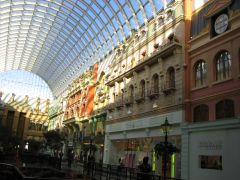
\includegraphics[width=.45\linewidth]{gfx/example_1}} \quad
        \subfloat[Pan ma signo.]
        {\label{fig:example-b}%
         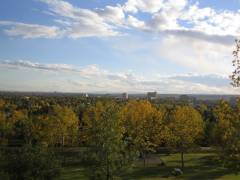
\includegraphics[width=.45\linewidth]{gfx/example_2}} \\
        \subfloat[Methodicamente o uno.]
        {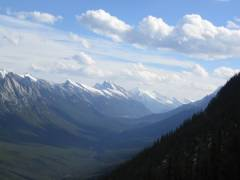
\includegraphics[width=.45\linewidth]{gfx/example_3}} \quad
        \subfloat[Titulo debitas.]
        {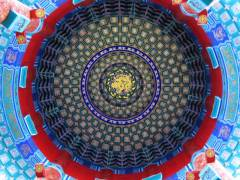
\includegraphics[width=.45\linewidth]{gfx/example_4}}
        \caption[Tu duo titulo debitas latente]{Tu duo titulo debitas
        latente. \ac{DRY}}\label{fig:example}
\end{figure}


%*****************************************
%*****************************************
%*****************************************
%*****************************************
%*****************************************

%\addtocontents{toc}{\protect\clearpage} % <--- just debug stuff, ignore
%%************************************************
\chapter{Math Test Chapter}\label{ch:mathtest} % $\mathbb{ZNR}$
%************************************************
Ei choro aeterno antiopam mea, labitur bonorum pri no. His no decore
nemore graecis. In eos meis nominavi, liber soluta vim cu. Sea commune
suavitate interpretaris eu, vix eu libris efficiantur.

\section{Some Formulas}
Due to the statistical nature of ionisation energy loss, large
fluctuations can occur in the amount of energy deposited by a particle
traversing an absorber element\footnote{Examples taken from Walter
Schmidt's great gallery: \\
\url{http://home.vrweb.de/~was/mathfonts.html}}.  Continuous processes
such as multiple
scattering and energy loss play a relevant role in the longitudinal
and lateral development of electromagnetic and hadronic
showers, and in the case of sampling calorimeters the
measured resolution can be significantly affected by such fluctuations
in their active layers.  The description of ionisation fluctuations is
characterised by the significance parameter $\kappa$, which is
proportional to the ratio of mean energy loss to the maximum allowed
energy transfer in a single collision with an atomic electron:
\graffito{You might get unexpected results using math in chapter or
section heads. Consider the \texttt{pdfspacing} option.}
\begin{equation}
\kappa =\frac{\xi}{E_{\textrm{max}}} %\mathbb{ZNR}
\end{equation}
$E_{\textrm{max}}$ is the maximum transferable energy in a single
collision with an atomic electron.
\[
E_{\textrm{max}} =\frac{2 m_{\textrm{e}} \beta^2\gamma^2 }{1 +
2\gamma m_{\textrm{e}}/m_{\textrm{x}} + \left ( m_{\textrm{e}}
/m_{\textrm{x}}\right)^2}\ ,
\]
where $\gamma = E/m_{\textrm{x}}$, $E$ is energy and
$m_{\textrm{x}}$ the mass of the incident particle,
$\beta^2 = 1 - 1/\gamma^2$ and $m_{\textrm{e}}$ is the electron mass.
$\xi$ comes from the Rutherford scattering cross section
and is defined as:
\begin{eqnarray*} \xi  = \frac{2\pi z^2 e^4 N_{\textrm{Av}} Z \rho
\delta x}{m_{\textrm{e}} \beta^2 c^2 A} =  153.4 \frac{z^2}{\beta^2}
\frac{Z}{A}
  \rho \delta x \quad\textrm{keV},
\end{eqnarray*}
where

\begin{tabular}{ll}
$z$          & charge of the incident particle \\
$N_{\textrm{Av}}$     & Avogadro's number \\
$Z$          & atomic number of the material \\
$A$          & atomic weight of the material \\
$\rho$       & density \\
$ \delta x$  & thickness of the material \\
\end{tabular}

$\kappa$ measures the contribution of the collisions with energy
transfer close to $E_{\textrm{max}}$.  For a given absorber, $\kappa$
tends
towards large values if $\delta x$ is large and/or if $\beta$ is
small.  Likewise, $\kappa$ tends towards zero if $\delta x $ is small
and/or if $\beta$ approaches $1$.

The value of $\kappa$ distinguishes two regimes which occur in the
description of ionisation fluctuations:

\begin{enumerate}
\item A large number of collisions involving the loss of all or most
  of the incident particle energy during the traversal of an absorber.

  As the total energy transfer is composed of a multitude of small
  energy losses, we can apply the central limit theorem and describe
  the fluctuations by a Gaussian distribution.  This case is
  applicable to non-relativistic particles and is described by the
  inequality $\kappa > 10 $ (\ie, when the mean energy loss in the
  absorber is greater than the maximum energy transfer in a single
  collision).

\item Particles traversing thin counters and incident electrons under
  any conditions.

  The relevant inequalities and distributions are $ 0.01 < \kappa < 10
  $,
  Vavilov distribution, and $\kappa < 0.01 $, Landau distribution.
\end{enumerate}


\section{Various Mathematical Examples}
If $n > 2$, the identity
\[
  t[u_1,\dots,u_n] = t\bigl[t[u_1,\dots,u_{n_1}], t[u_2,\dots,u_n]
  \bigr]
\]
defines $t[u_1,\dots,u_n]$ recursively, and it can be shown that the
alternative definition
\[
  t[u_1,\dots,u_n] = t\bigl[t[u_1,u_2],\dots,t[u_{n-1},u_n]\bigr]
\]
gives the same result.  

%*****************************************
%*****************************************
%*****************************************
%*****************************************
%*****************************************

%\include{multiToC} % <--- just debug stuff, ignore for your documents

% \graffito{} für Randbemerkungen
%************************************************
\chapter{Einleitung}\label{kap:eileitung}
%************************************************

Bei der Entwicklung in Richtung \gls{industrie40} werden Industrieanlagen und andere physische Systeme zur effizienten Auslastung und Energienutzung über einen zunehmenden Kommunikationsfluss miteinander vernetzt. Verkabelte Systeme sind in den meisten Anwendungsfällen zu unflexibel oder gar nicht realisierbar, sodass auf kabellose Kommunikation ausgewichen werden muss. Moderne eingebettete Systeme stellen hierbei die nötige Performanz zur Verfügung. So entstehen \acfp{cps}, die eine Dezentralisierung komplexer Systeme ermöglichen und zu steigender Flexibilität führen. In großen Logistiklagern bieten vernetzte Frachtcontainer ein hohes Maß an Selbstorganisation, wie die Überwachung des Frachtgutes oder die automatische Inventarisierung \citep{inBin}. Es entsteht ein \acf{wsn}, in welchem die Frachtcontainer als Netzwerkknoten, den so genannten \glspl{node}, fungieren.

In Logistiklagern ist nur der Betrieb von besonders energieeffizienten oder gar energieautarken Lösungen denkbar, da Batteriewechsel oder Akku-Ladevorgänge die Dynamik und Zuverlässigkeit des gesamten Lagers negativ beeinträchtigen. Aus diesem Grund müssen derartige Systeme besonders sparsam mit der verfügbaren Energie haushalten. Eine Schlüsselrolle stellt in diesem Zusammenhang die Funkkommunikation dar, die im Verhältnis zur übrigen Intelligenz der Frachtcontainer besonders energieintensiv ist \citep{inBin}\citep{inBinTestbed}\citep{xmac}.

Folglich müssen Übertragungen zuverlässig übermittelt werden. Diesem Ziel wirken in einem Logistiklager jedoch zahlreiche Faktoren entgegen: Z.B. erhöht die sehr hohe Teilnehmerzahl die Interferenz auf den einzelnen Übertragungsstrecken, was zu massiven Übertragungskollisionen führt \citep{inBinTestbed}\citep{GreenOrbs}.

Aktuelle Forschungen beschäftigen sich sowohl mit den speziellen Anforderungen intelligenter, vernetzter Logistiklager \citep{inBinTestbed}, als auch mit Skalierungseffekten von Sensornetzen allgemein \citep{GreenOrbs}. Die bei  großskaligen Anwendungen  inhärente Konkurrenz der Teilnehmer wird hierbei wiederholt als wesentliches Problem benannt.

\section{Motivation}
Auf Grund der genannten hohen Anzahl an konkurrierenden \glspl{node} innerhalb eines Netzwerkes ist der Kanalzugriff ein kritischer Punkt im Bezug auf eine verlässliche und effiziente Funkkommunikation. Eine Netzwerküberlastung kann aus einem hohen Datenaufkommen einzelner \glspl{node} oder aus einer großen Zahl konkurrierender \glspl{node} innerhalb eines \ac{wsn} resultieren. Kommen beide Fälle zusammen, wird das Netzwerk noch stärker beansprucht. Schlagen Übertragungen fehl, müssen sie ggf. wiederholt werden, was die Netzlast weiter erhöht und sich negativ auf den Energieverbrauch der \glspl{node} auswirkt.

Diese Arbeit beschäftigt sich daher mit der Entwicklung und Bewertung eines geeigneten Kanalzugriffverfahrens für derartige Logistikszenarien.
Dabei sollen die folgenden Fragestellungen beantwortet werden:
\begin{enumerate}
	\item Wo stoßen gängige Kanalzugriffverfahren an ihre Grenzen?
	\item Wie können sie hinsichtlich ihrer Leistungsstärke modifiziert werden?
	\item Welche Einschränkungen ergeben sich daraus?
	\item Welchen Einfluss nimmt das Kanalzugriffverfahren auf den Energieverbrauch?
\end{enumerate}

\section{Lösungsansatz}
Der Lösungsansatz ist die Analyse des \acf{csma} Verfahrens aus dem \gls{802154} Protokoll. Mit Hilfe eines Simulationsmodells wird der Algorythmus zum Kanalzugriff zunächst mit Standardparametern unter den Rahmenbedingungen eines Logistiklagers untersucht. Im Anschluss werden Auswirkungen der Variation  \acs{csma}-Parameter simuliert. Zur Beurteilung der Energieeffizienz fließen Messdaten realer \gls{transceiver} in die Simulation ein. Durch eine prototypische Implementierung dieses Ansatzes werden die Simulationsergebnisse im Feldversuch hinsichtlich der Zuverlässigkeit und des Energieverbrauchs validiert.

\section{Struktur der Arbeit}
TODO: aktualisieren

Die Arbeit gliedert sich wie folgt. \autoref{kap:verwandtearbeiten} zeigt die Ergebnisse bisheriger Untersuchungen auf und führt hin zur Motivation, welche in \autoref{kap:motivation} ausgeführt wird. Grundlegend für die eigentliche Untersuchung beschreibt \autoref{kap:sensornetzwerkefuerlogistiklager} die Struktur des analysierten Szenarios. In \autoref{kap:zugriffverfahren} werden zwei standardisierte Kanalzugriffsverfahren unter Berücksichtigung des Energieverbrauchs diskutiert. Es folgt eine umfassende Beschreibung des verwendeten Simulationsmodells 

TODO: weitere Beschreibung der Kapitel vervollständigen.

%*****************************************
%*****************************************
%*****************************************
%*****************************************
%*****************************************





%************************************************
\chapter{Grundlagen}\label{kap:grundlagen}
%************************************************
In diesem Kapitel werden die erforderlichen Grundlagen beschrieben, auf denen die Auslegung der Simulation, der Bewertung der Ergebnisse und die prototypische Implementierung aufbauen. Dabei gliedert sich das Kapitel in 5 Teile: \autoref{kap:grundlagen_sec:funk} und \autoref{kap:grundlagen_sec:protokolle} behandeln Grundzüge der Funkkommunikation sowie den damit verbunden Verarbeitungsvorschriften für die Systemsoftware, den Protokollen. Es folgt \autoref{kap:grundlagen_sec:energieverbrauch} mit relevanten Faktoren und Diagnosemöglichkeiten hinsichtlich des Energieverbrauchs bei Funkkommunikation. \autoref{kap:grundlagen_sec:simulation} gibt eine Einführung in ereignisorientierte Simulationen. In \autoref{kap:grundlagen_sec:hardware} werden die verwendeten Hardwareplattformen und ihre Besonderheiten vorgestellt.

\section{Funkkommunikation}\label{kap:grundlagen_sec:funk}

\begin{figure}[bth]
        \myfloatalign
        {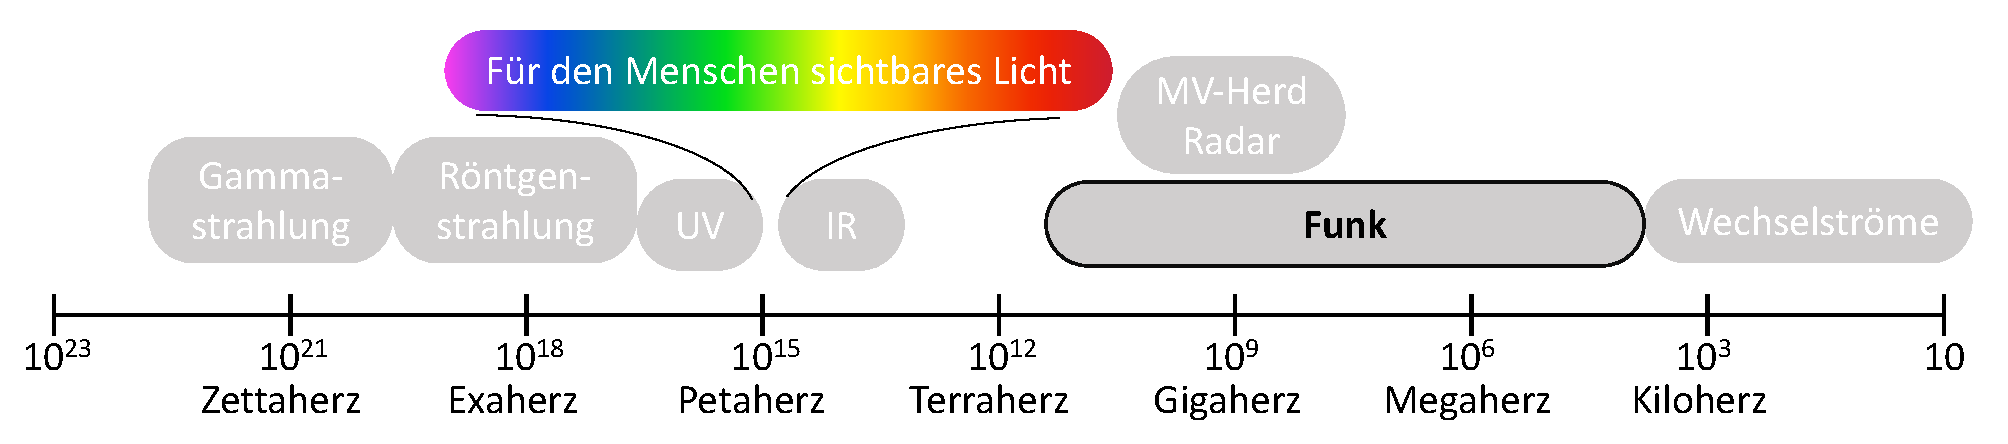
\includegraphics[width=1\linewidth]{gfx/Spektrum}} 
        \caption[Spektrum]{Einordnung von Funkwellen im elektromagnetischen Spektrum}\label{fig:spektrum}
\end{figure}

Funkkommunikation ist die Übertragung von Informationen durch elektromagnetische Wellen. Dabei stehen Funkwellen verschiedener Frequenzen als Übertragungsmedium zu Verfügung. Abschnitte des Funkspektrums werden Bänder genannt. Ein Frequenzband kann je nach Anwendung in weitere Abschnitte, den sogenannten Kanälen, unterteilt werden. Der Radio- und Fernsehrundfunk, der Mobilfunk oder Satellitenübertragungen sind typische Beispiele. Aber auch \acs{wlan}, \gls{bluetooth}, schnurlose Telefone, Rauchmelder oder \acsp{wsn} nutzen Funkwellen zum Informationsaustausch. Eine Einordnung der Funkwellen im gesamten elektromagnetischen Spektrum ist in \autoref{fig:spektrum} zu sehen. Den verschiedenen Anwendungen sind dabei bestimmte Frequenzabschnitte zugeordnet.  Diese Zuordnung ist teilweise mit kostenpflichtigen Lizenzen versehen, die in Deutschland die Bundesnetzagentur verwaltet. So werden \zB einzelne Frequenzbereiche an Mobilfunkanbieter versteigert. Neben den lizensierten Bändern, stehen auch Bereiche speziell für den Einsatz in Industrie, Wissenschaft und Medizin zur Verfügung. Diese Frequenzen werden im \gls{ism} Band zusammengefasst. Die in Deutschland zur Verfügung stehenden Bereiche befinden sich u.a. im $434MHz$ Band, im $2,4GHz$ Band und im $5,7 GHz$ Band. Der $868MHz$ ist vornehmlich für Alarmfunkanlagen vorgesehen. Der Bereich $868,6MHz - 868,7MHz$ steht jedoch auch für allgemeinen Datenaustausch zur Verfügung \citep{ISMBand}.

\subsection{Freiraumausbreitung}\label{kap:grundlagen_sec:wellenausbreitung}

\begin{figure}[bth]
        \myfloatalign
        {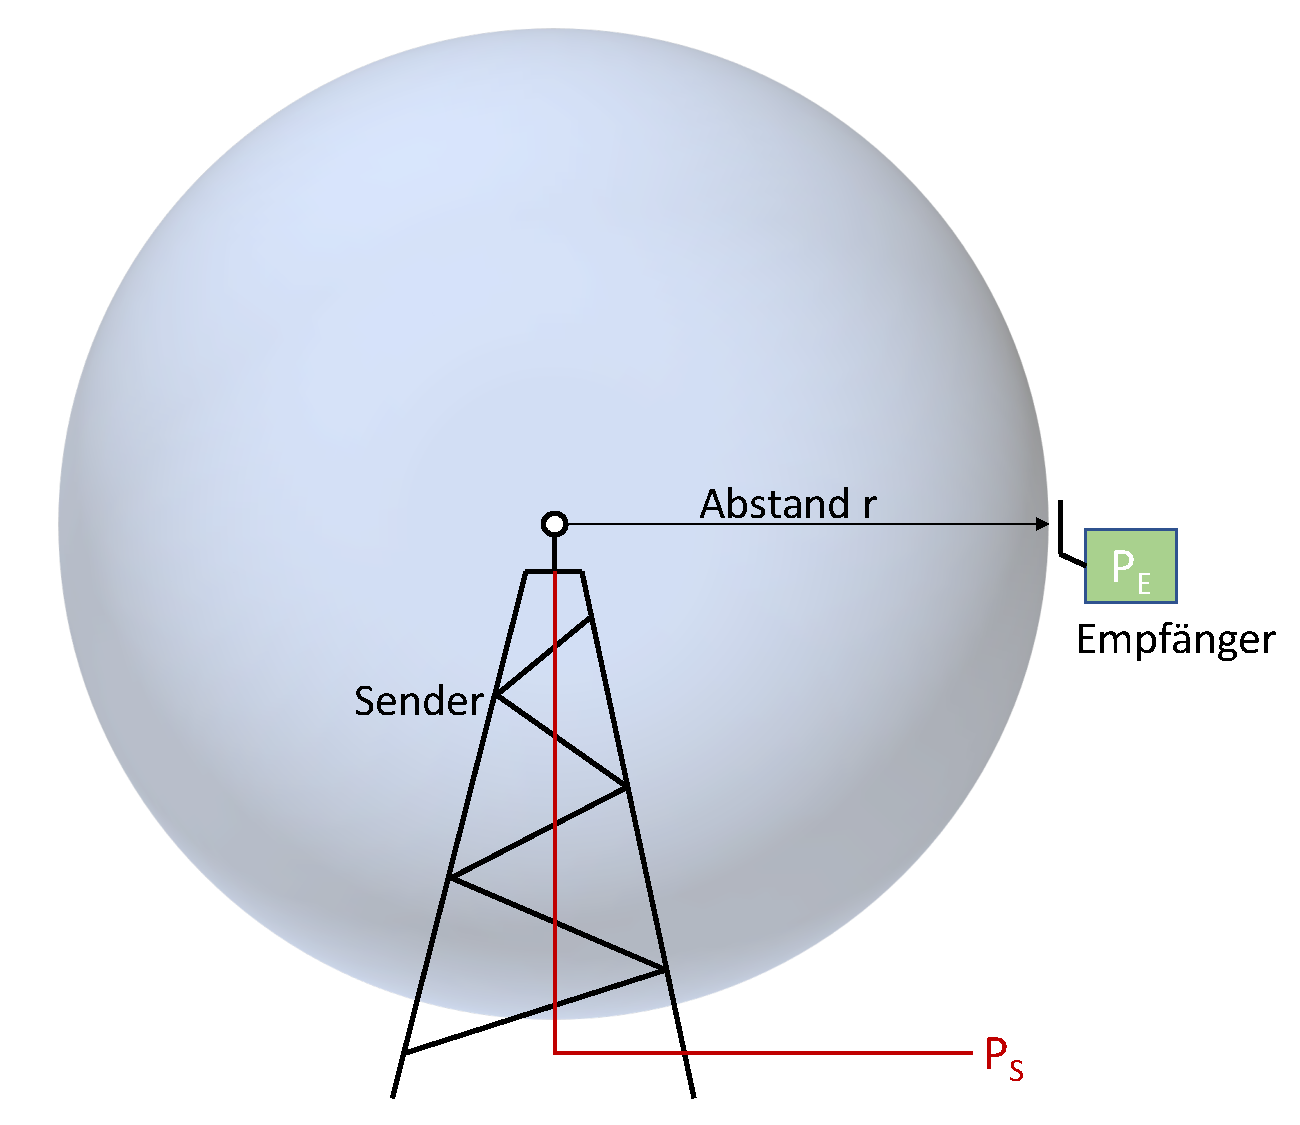
\includegraphics[width=0.6\linewidth]{gfx/Funkausbreitung}} 
        \caption[Ausbreitung]{Idealisierte Funkwellenausbreitung mit isotropen Antennen}\label{fig:Isotropstrahler}
\end{figure}

Zur Beschreibung der Wellenausbreitung seien zunächst isotrope Strahler betrachtet, also Antennen, von denen sich die Funkwellen mit der Lichtgeschwindigkeit $c$ gleichmäßig in alle Raumrichtungen ausbreiten, wie in \autoref{fig:Isotropstrahler} skizziert. Wird ein zu übertragenes Signal mit der Leistung $P\textrm{S}$ in eine solche Sendeantenne eingespeist, so verteilt sich diese Leistung im Abstand $r$ auf die Fläche einer Kugel mit Radius $r$. Die Leistungsdichte an einem beliebigen Punkt im Umfeld des Senders beträgt:
\begin{equation}
{S = \frac{P_\textrm{S}}{A_\textrm{Kugel}} = \frac{P_S}{4{\pi}r^2}}
\label{eq:leistungsdichte}
\end{equation}
Um der elektromagnetischen Welle Leistung zu entnehmen, muss die Empfangsantenne im mathematischen Sinn eine Fläche besitzen, die von der Leistungsdichte durchsetzt wird. Diese wird Antennenwirkfläche $A_W$ genannt.
\begin{equation}
{P_E = S  \cdot A_W}
\label{eq:pe1}
\end{equation}
Die Antennenwirkfläche ist nicht die geometrische Fläche der Antenne, sondern ein frequenzabhängiger Wert. Bei einer isotropen Antenne ist die Antennenwirkfläche definiert zu:
\begin{equation}
{A_W = \frac{c^2}{4{\pi}f^2}}
\label{eq:aw}
\end{equation}
Nach Einsetzen von \autoref{eq:aw} und \autoref{eq:leistungsdichte} in \autoref{eq:pe1} ergibt sich die Empfangsleistung:
\begin{equation}
{P_E = \frac{P_S}{4{\pi}r^2} \cdot \frac{c^2}{4{\pi}f^2} = P_S \cdot \left(\frac{c}{4{\pi}rf}\right)^2}
\label{eq:pe2}
\end{equation}

\begin{table}
    \myfloatalign
  \begin{tabularx}{0.5\textwidth}{Xll} \toprule
    \tableheadline{Abstand} & \tableheadline{$P_E$} \\ \midrule
    $10m$ & $0,57mW$ \\
    $20m$ & $0,14mW$ \\
    $30m$ & $0,06mW$ \\
    \bottomrule
  \end{tabularx}
  \caption[Empfangsleistung]{Empfangsleistung bei Freiraumausbreitung und isotropen Rundstrahler mit der Sendeleistung $1Watt$ bei $100MHz$}  \label{tab:empfangsleistung}
\end{table}

In \autoref{tab:empfangsleistung} sind exemplarisch die Empfangsleistungen einer Übertragung bei $100Mhz$ und eine Sendeleistung von $1Watt$ eingetragen. Dabei wird ersichtlich, dass am Empfänger nur noch ein Bruchteil der ursprünglichen Signalleistung zur Verfügung steht.
Die Verringerung der Sendeleistung wird Dämpfung genannt und als logarithmisches Maß in Dezibel angegeben. Sie ist das Verhältnis von $P_S$ zu $P_E$. Nach \autoref{eq:pe2} ergibt sich die \emph{Freiraumdämpfung} $F$ zu:

\begin{equation}
{F = 10\lg \left(\frac{P_S}{P_E}\right) = 10\lg\left(\frac{4{\pi}rf}{c}\right)^2 }
\label{eq:freiraumdämpfung}
\end{equation}

In \autoref{fig:Isotropstrahler} ist die Freiraumdämpfung für drei verschiedene Frequenzen des \gls{ism}-Bands über die Entfernung zwischen Sender und Empfänger aufgetragen. Es ist gut zu erkennen, dass hohe Frequenzen stärker gedämpft werden als niedrige.

\begin{figure}[bth]
        \myfloatalign
        {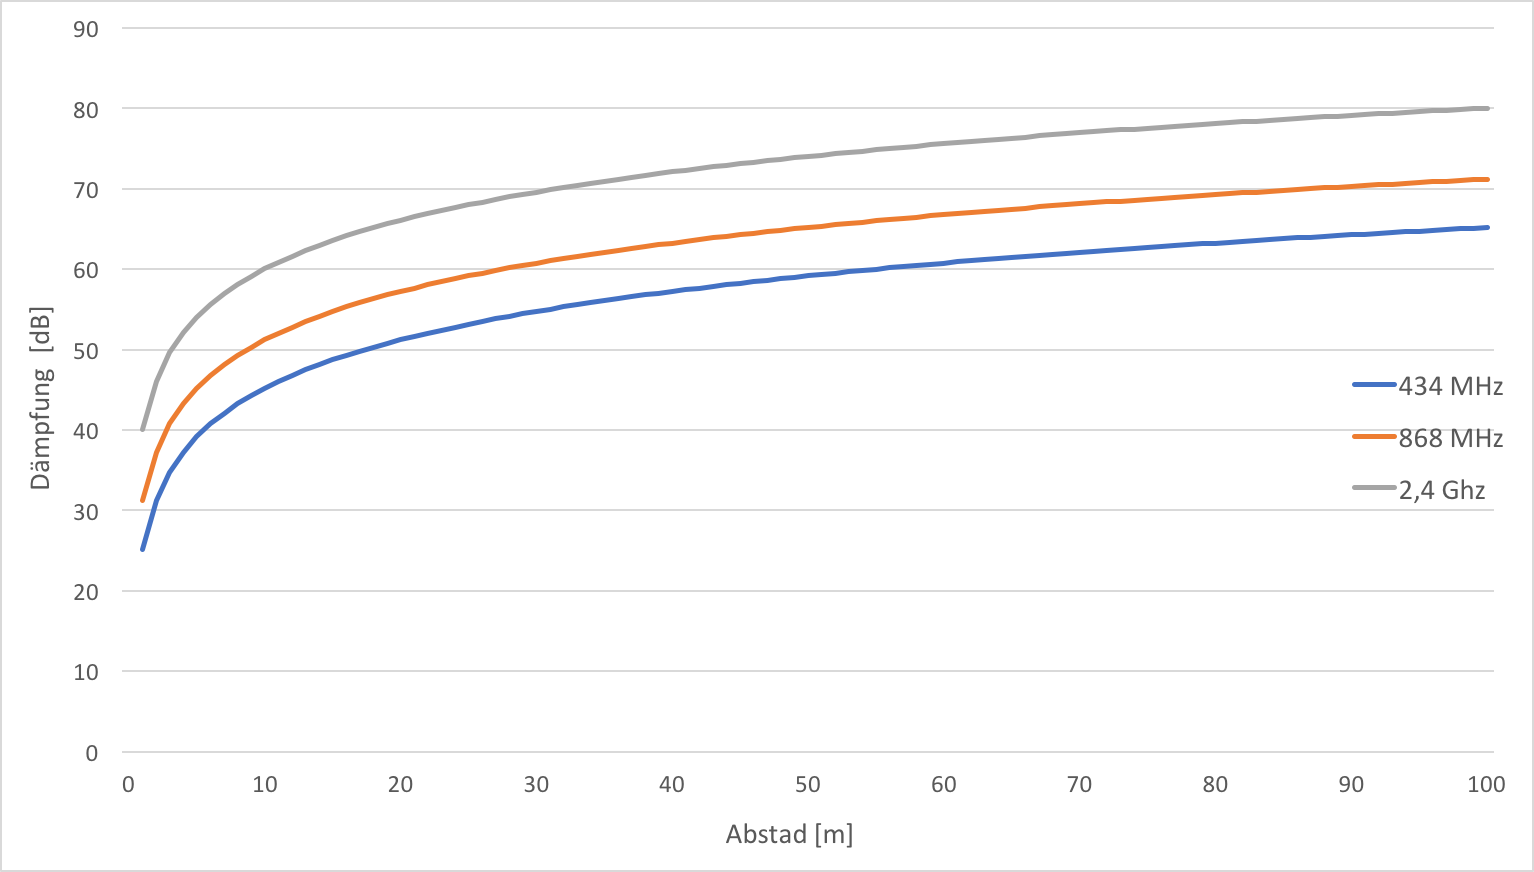
\includegraphics[width=1\linewidth]{gfx/Freiraumdaempfung}} 
        \caption[Freiraumdämpfung]{Freiraumdämpfung bei verschiedene Frequenzen}\label{fig:Isotropstrahler}
\end{figure}

Bei realen Antennen entspricht die abgestrahlte Leistung auf Grund von \zB ohmschen Verlusten innerhalb der Antenne, nicht der eingespeisten Leistung. Dieser Verlustfaktor, also das Verhältnis von abgestrahlter zu eingespeister Leistung wird durch den Antennenwirkungsgrad $\eta$ ausgedrückt. 

In der Regel strahlen Antennen nicht gleichmäßig in alle Raumrichtungen, wie in \autoref{fig:Isotropstrahler}. Antennen können speziell so konzipiert werden, dass sie die abgestrahlte Leistung in bestimmten Richtungen bündeln. Es kann \zB in einigen Anwendungen sinnvoll sein, wenn die Sendeantenne weniger stark nach oben und nach unten strahlt, dafür umso mehr in die Breite. Das ist bei Dipolantennen der Fall. Ein weiteres Beispiel ist der Richtfunk. Hierbei wird die Strahlungsleistung in eine Raumrichtung maximiert. Parabolantennen weisen dieses Merkmal auf. Zur Berechnung wird diese Eigenschaft im Richtfaktor $D$ einer Antenne ausgedrückt. Es ist das Verhältnis der Leistungsdichte $S_max$ in der Hauptstrahlrichtung der Antenne zu der Strahlungsleistung $S$ einer gleichförmig strahlenden Antenne an gleicher Stelle.

Die Größen $\eta$ und $D$ charakterisieren eine Antenne und werden im Antennengewinn $g$ zusammengefasst.
 \begin{equation}
{g = \eta \cdot D}
\label{eq:antennengewinn}
\end{equation}

Unter Berücksichtigung des Antennengewinns von Sende- und Empfangsantenne kann \autoref{eq:pe2} zur Antennengleichung für Freiraumausbreitung erweitert werden:
\begin{equation}
{P_E = P_S \cdot g_S \cdot g_E \cdot \left(\frac{c}{4{\pi}rf}\right)^2}
\label{eq:pe3}
\end{equation}

\subsection{Rauschen}\label{kap:grundlagen_sec:rauschen}
Ein Signal wird während der Übertagung durch äußere Störungen beeinträchtigt, die \zB durch andere Funksender oder die kosmische Hintergrundstrahlung hervorgerufen werden. Die Überlagerung aller störenden äußeren Einflüsse wird als Rauschen bezeichnet. Rauschen kann daher als Überlagerung vieler elektromagnetischer Wellen unterschiedlicher Frequenzen und mit unterschiedlichen Signalamplituden aufgefasst werden. Um diese Effekte auf dem Funkkanal bei Übertragung zu berücksichtigen, ist ein Kanalmodell notwendig.  Unter der Annahme, dass die einzelnen Schwingungen völlig unabhängig von einander sind, liegt ein \acf{awgn} vor und man spricht von einem \acs{awgn}-Kanal.
\begin{figure}[bth]
        \myfloatalign
        {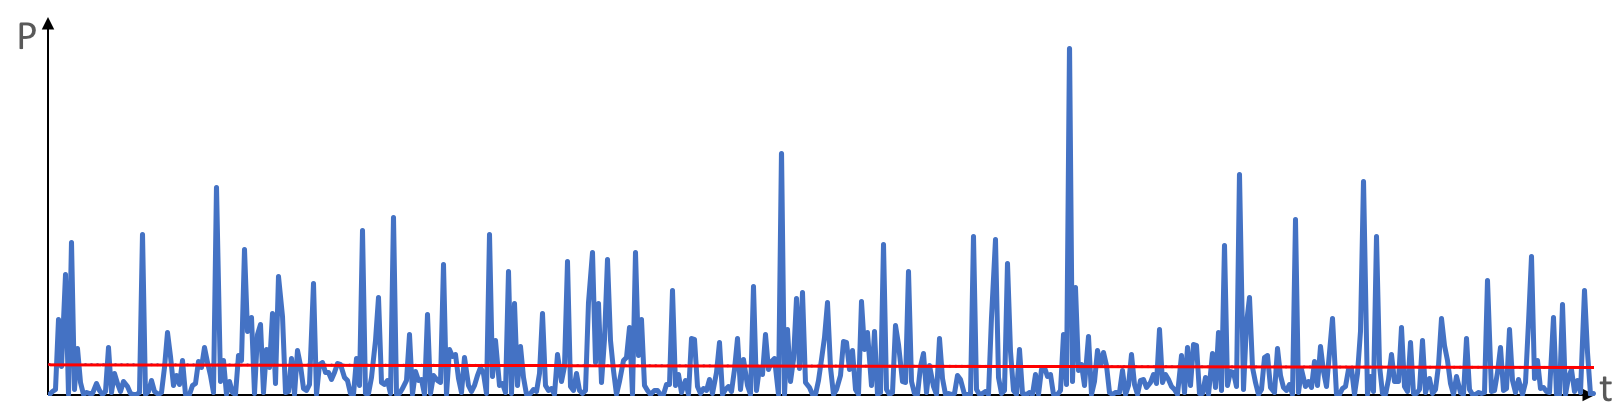
\includegraphics[width=1\linewidth]{gfx/AWGN}} 
        \caption[AWGN]{Zeitlicher Verlauf der momentanen Rauchleistung eines \acs{awgn}-Kanals}\label{fig:awgn}
\end{figure}

Bei diesem Kanalmodell sind die Signalamplituden des Rauschsignals normalverteilt, d.h. der Großteil der vorkommenden Amplituden weicht nur wenig von dem durchschnittlichen Wert ab, wohingegen extreme Amplituden nur selten vorkommen. Der Verlauf der Rauschleisung eines solchen Signals ist in \autoref{fig:awgn} dargestellt. Weiterhin ist die Rauschleistungsdichte $N_0$ bei einem \acs{awgn}-Kanal über alle Frequenzen konstant. Die Rauschleistung $N$ eines Kanals mit der Bandbreite $B$ ergibt sich dann zu:
\begin{equation}
{N = N_0 \cdot B}
\label{eq:pe3}
\end{equation}
Wie in \autoref{kap:grundlagen_sec:wellenausbreitung} beschrieben, fällt die Signalleistung bis zum Ort des Empfängers stark ab. Damit ein Nutzsignal mit der Signalleistung $P$ vom Empfänger dedektiert werden kann, muss $P$ größer als die vorherrschende Rauschleistung $N$ sein. Der Abstand von $N$ zu $P$ wird als \emph{Störabstand} oder als \acf{snr} bezeichnet und logarithmisch in Dezibel angegeben.
\begin{equation}
{SNR = 10\lg\left(\frac{P}{N}\right) = 10\lg\left(\frac{P}{N_0 \cdot B}\right)}
\label{eq:pe3}
\end{equation}




\subsection{Modulation}\label{kap:grundlagen_sec:modulation}
Bei einer digitalen Datenübertragung werden die zu übermittelnden Informationseinheiten als Symbole bezeichnet. Die Geschwindigkeit, mit der Symbole übertragen werden, ist die Symbolrate und hat die Einheit \emph{Baud}. In einem Symbol können mehrere Bits zusammengefasst sein. Die Anzahl der Bits pro Symbol bestimmt den Modulationsindex $M$. In \autoref{fig:modulation} ist eine Bitfolge mit Modulationsindex $M=2$ und $M=4$ gegenübergestellt.
\begin{figure}[bth]
        \myfloatalign
        \subfloat[$M = 2$]
        {\label{fig:nachrichten-a}%
         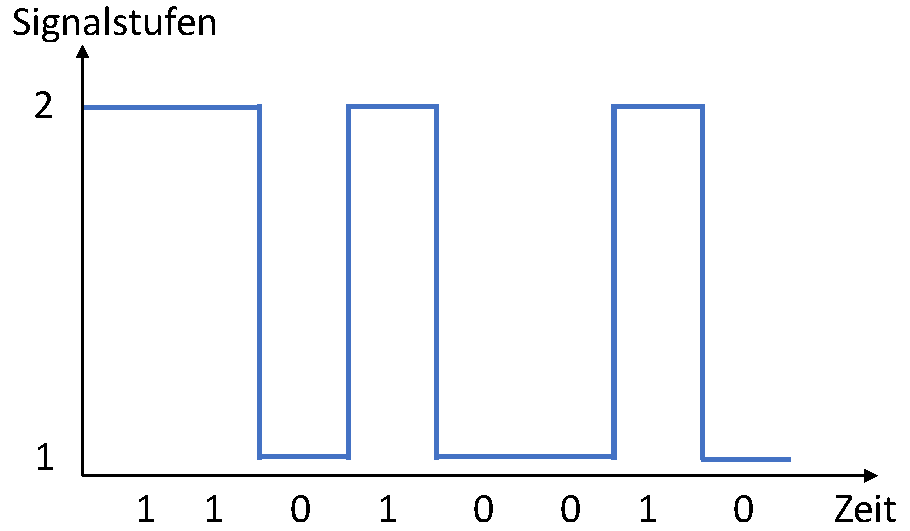
\includegraphics[width=0.5\linewidth]{gfx/ModulationA}} 
        \subfloat[$M = 4$]
        {\label{fig:nachrichten-b}%
        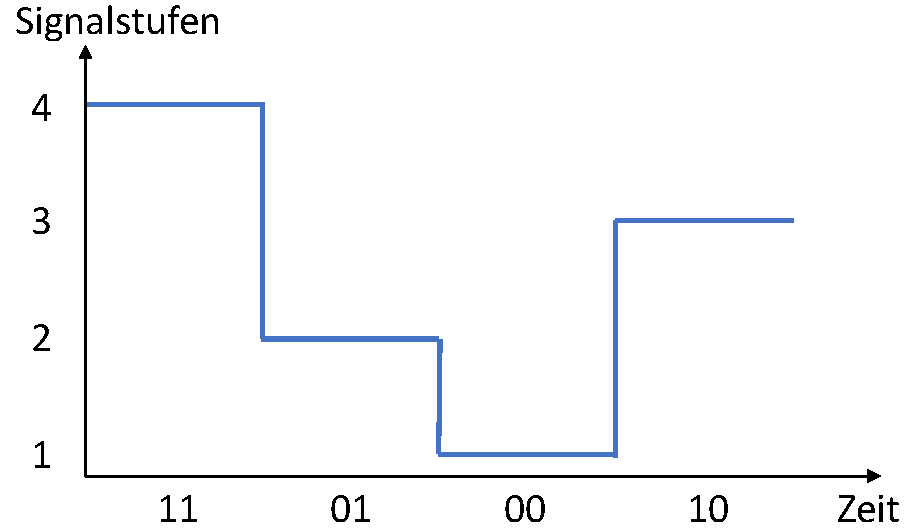
\includegraphics[width=0.5\linewidth]{gfx/ModulationB}} 
        \caption[Moduationsstufe]{Gegenüberstellung einer Bitfolge bei verschiedenen Signalstufen. a) Ein Symbol entspricht einem Bit b) In einem Symbol werden zwei Bits zusammengefasst, es gibt vier Signalstufen}\label{fig:modulation}
\end{figure}
Es ist zu erkennen, dass es bei einem Bit pro Symbol zwei unterschiedliche Symbole gibt, bei zwei Bits pro Symbol dagegen vier unterschiedliche Symbole. Es gilt der Zusammenhang:
\begin{equation}
{M = Anzahl_\textrm{Bits/Symbol}^2}
\label{eq:m}
\end{equation}
Die Anzahl der übertragenen Bits pro Sekunde steigt daher bei größerem Modulationsindex. Für die Datenrate $R$ gilt:
\begin{equation}
{R = \log_{2}(M)}
\label{eq:R}
\end{equation}

Die digitalten Daten müssen für die Übertragung auf ein analoges Signal, den sogenannten Träger, modelliert werden. Dies kann \zB durch die Manipulation der Amplitude, der Frequenz oder der Phasenlage einer Sinusschwingung erzielt werden. Dieser Vorgang wird auch als Umtastung bezeichnet. Besonders robust gegen Überlagerungen anderer Signale ist die \acf{fsk}. Hierbei wird die Frequenz der Trägerschwingung in Abhängigkeit des zu übertragenden Symbols leicht verändert, wie in \autoref{fig:fsk} angedeutet. In dem abgebildeten Beispiel, wird nur ein Bit pro Symbol übertragen, d.h der Modulationsindex $M$ ist gleich zwei. Man spricht daher in dem Fall von einer 2-\acs{fsk}.

\begin{figure}[bth]
        \myfloatalign
        {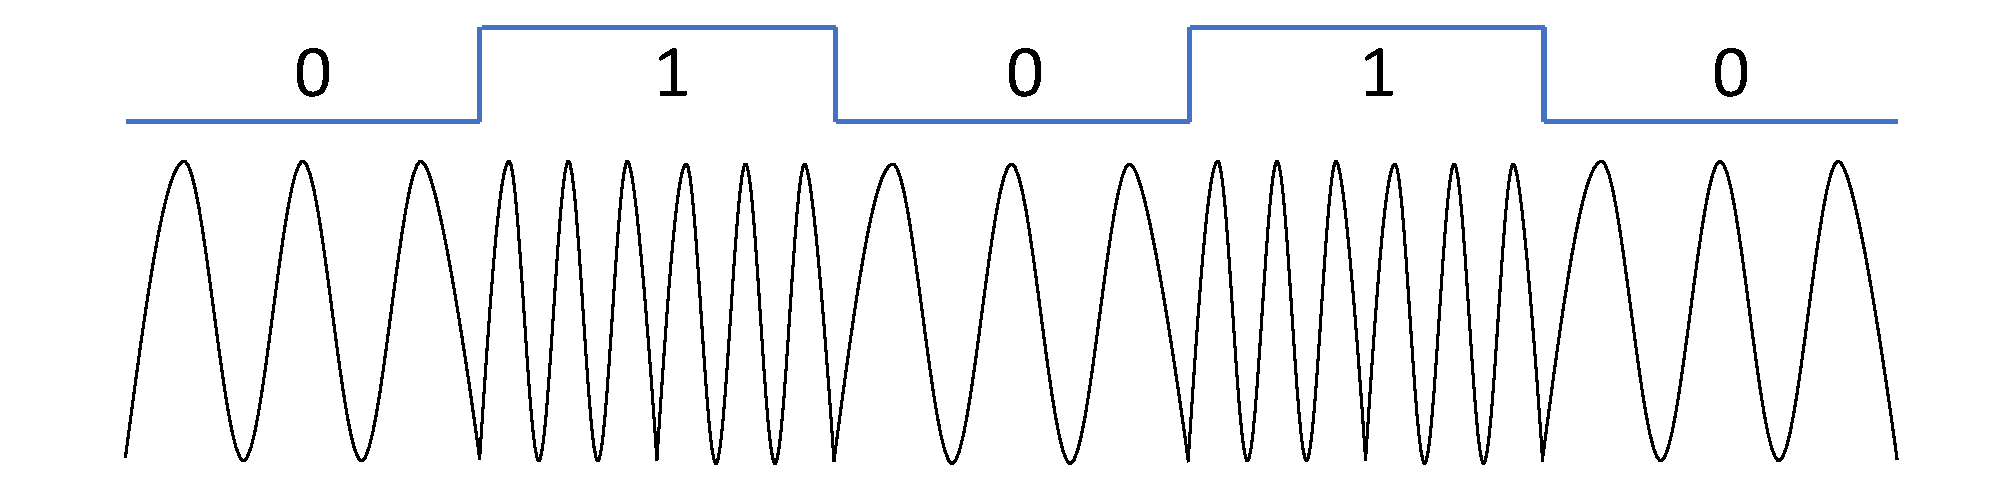
\includegraphics[width=1\linewidth]{gfx/FSK}} 
        \caption[FSK]{Ein digitlaes Signal wird mittels \acs{fsk} mit $M=2$ auf ein Trägersignal modelliert. Dabei wird die Frequenz des Trägers variiert.}\label{fig:fsk}
\end{figure}

Abrupte Übergänge im zeitlichen Signalverlauf führen zu einem breiten Frequenzspektrum. Daher kann bei einer Datenübertragung nicht beliebig schnell zwischen zwei Symbolen umgeschaltet werden, die verfügbare Bandbreite $B$ des Funkkanals begrenzt die Datenrate. Die theoretisch maximal erreichbare Datenrate ist nach Nyquist:
\begin{equation}
{R_{max} = 2 \cdot B \cdot \log_{2}(M)}
\label{eq:nyquist}
\end{equation}

Nach \autoref{eq:R} lässt sich die Datenrate durch Erhöhen des Modulationsindexes steigern. Störungen auf dem Funkkanal erhöhen jedoch dabei die Wahrscheinlichkeit, dass die verschiedenen Symbole am Empfänger nicht mehr korrekt voneinander unterscheiden werden können. Das Shannon-Hartley-Gesetz gibt die maximale Datenrate für eine Übertragung auf einem verrauschten Kanal mit der Rauschleistung $N$ an, bei der die Wahrscheinlichkeit einer fehlerfreien Übertragung noch größer Null ist.
\begin{equation}
{R_{max} =  B \cdot \log_{2}(1 + \frac{P_\textrm{Signal}}{N})}
\label{eq:shannon}
\end{equation}

Ein Datenstrom wird üblicherweise nicht direkt in die Sendefrequenz umgetastet, sondern zunächst auf eine Zwischenfrequenz. Diese wird im Anschluss auf die tatsächliche Sendefrequenz, \zB $868MHz$, gemischt. 

\autoref{kap:grundlagen_sec:wellenausbreitung} hat gezeigt, dass Übertragungen bei  hohen Frequenzen wegen der stärkeren Dämpfung Nachteile in der Ausbreitung  gegenüber niedrigeren Frequenzen aufweisen. In diesem Abschnitt wird deutlich, dass hohe Frequenzen dafür bezüglich hoher Datenraten geeigneter sind. In den höheren Frequenzbereichen steht den einzelnen Kanälen mehr Bandbreite zur Verfügung, was nach \autoref{eq:shannon} eine größere Datenrate erlaubt.

\subsection{Kanalausnutzung}\label{kap:grundlagen_sec:kanalausnutzung}
Um einen Funkkanal für mehrere Benutzer zugänglich zu machen und dabei dennoch eine funktionierende Kommunikation zu gewährleisten, ist ein Zugriffsverfahren notwendig. Nachfolgend sind dazu verschiedene Techniken aufgeführt.
\begin{description}
\item[FDMA] Beim \acf{fdma} wird jedem Nutzer ein eigenes Teilband innerhalb des vorgesehenen Frequenzbereiches zugeordnet, sodass im Endeffekt die Übertragungen der einzelnen Benutzer in parallelen Kanälen stattfinden. Es ist darauf zu achten, dass sich die einzelnen Kanäle nicht gegenseitig stören. Dies kann \zB durch das Hinzufügen von Schutzkanälen realisiert werden, in denen keine Übertragung stattfindet. Dieses Verfahren schränkt die Datenrate der Teilnehmer wegen der geringeren Bandbreite ein (vgl. \autoref{kap:grundlagen_sec:modulation}).

\item[TDMA] Beim \acf{tdma} wird nicht das Funkspektrum als begrenzte Ressource aufgeteilt, sondern die Zeit. Jedem Teilnehmer wird ein eigener Zeitschlitz zugeteilt, in dem dieser senden darf. Dieses Verfahren erfordert eine genaue Synchronisierung aller Teilnehmer im Netzwerk.

\item[CDMA] Bei dem Verfahren mit \acf{cdma} wird ein schmalbandiges Signal  auf einen sehr viel breiteren Frequenzbereich gespreizt. Diese Spreizung erfolgt für jeden Nutzer nach einem individuellen Muster. Die breitbandigen Signale sind unempfindlich gegen schmal- und breitbandige Störungen. Somit können sie trotz Überlagerung am Empfänger wieder von einander getrennt werden. Dazu verwendet der Empfänger jeweils das gleiche Spreizmuster, wie der Sender.

\item[SDMA] Beim \acf{sdma} werden den Nutzern verschiedene räumliche Sektoren zugeteilt. Dies kann mittels der Richtcharakteristik von geeigneten Antennen erreicht werden (vgl. \autoref{kap:grundlagen_sec:wellenausbreitung}).

\item[CSMA] \acf{csma1} ist ein dezentrales, asymmetrisches Verfahren. Das bedeutet, dass keine zentrale Koordination oder Synchronisation der Nutzer nötig ist. Die Nutzer beanspruchen nach einem bestimmten Algorithmus das alleinige Zugriffsrecht auf den Kanal. Zur Koordination beobachten die Nutzer dabei den Kanal. Eine detaillierte Beschreibung solcher Verfahren erfolgt in \autoref{kap:zugriffsverfahren}.
\end{description}

\subsubsection{Hidden Station Problem}\label{kap:grundlagen_sec:hiddenstation}
Ein Effekt, der bei der zuletzt genannten Technik zu beachten ist, ist das \gls{hiddenstation}. Dieser tritt beim Abhören des Funkkanals auf, wenn es Nutzer im Netzwerk gibt, die außerhalb der Reichweite anderer Nutzer liegen.
\begin{figure}[bth]
        \myfloatalign
        {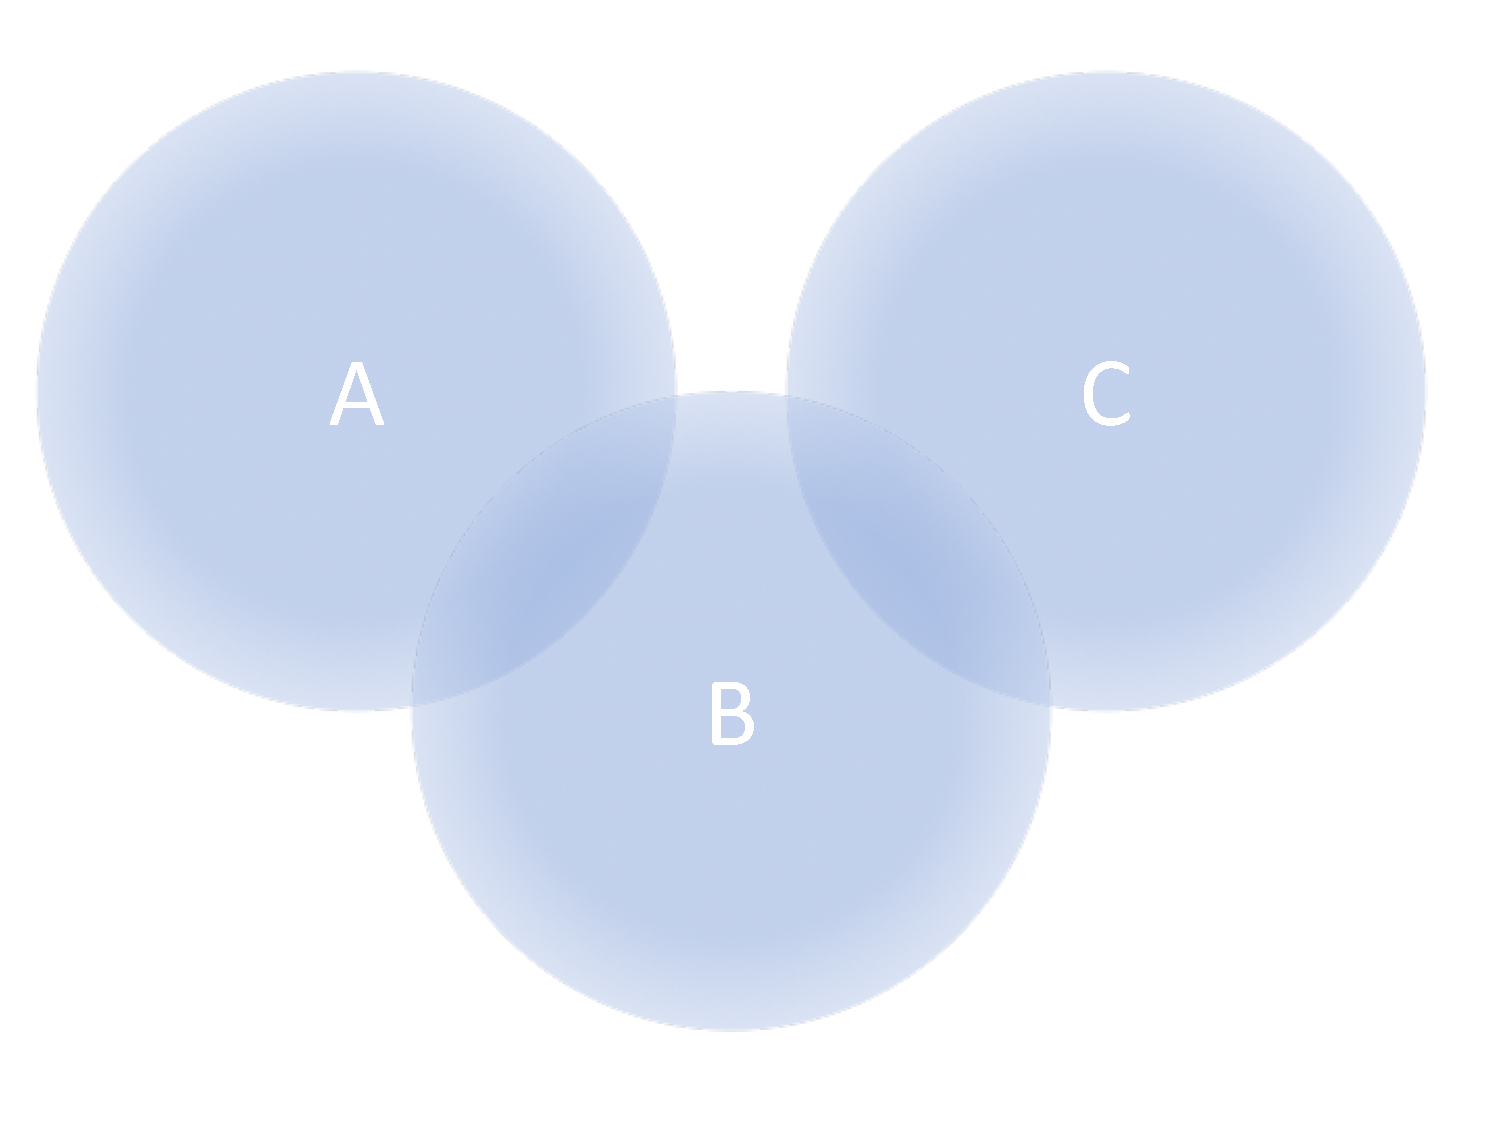
\includegraphics[width=0.7\linewidth]{gfx/HiddenStation}} 
        \caption[Hidden Station]{Veranschaulichung des \gls{hiddenstation} bei drei Nutzern. Abgebildet sind drei Funksender A, B und C und ihre Sendereichweiten}\label{fig:hiddenstation}
\end{figure}
\autoref{fig:hiddenstation} zeigt drei Nutzer mit den jeweiligen Funkreichweiten. Möchte in diesem Szenario Nutzer A an Nutzer B senden, während Nutzer B gerade inaktiv ist, startet A die Übertragung. Wenn nun gleichzeitig auch Nutzer C an Nutzer B senden möchte, ist dieser nicht in der Lage, die Aktivität von A zu detektieren, da Nutzer C außerhalb der Reichweite von Nutzer A liegt. In der Folge kollidieren die Übertragungen von Nutzer A und Nutzer C.

Ein Ansatz, der diesem Problem entgegenwirkt, ist das Versenden von \acs{rts}- und \acs{cts}-Nachrichten. In dem beschriebenen Beispiel würde Nutzer A zunächst eine \acs{rts}-Nachricht versenden, woraufhin Nutzer B mit einer \acs{cts}-Nachricht antwortet. Somit findet bei Nutzer B auch eine Aktivität statt, die Nutzer C detektieren kann.

\section{Kommunikationsprotokolle}\label{kap:grundlagen_sec:protokolle}
In den vorangegangen Abschnitten wurden bereits einige Verfahren beschrieben, die für die erfolgreiche Übermittlung von Informationen in einem Funknetzwerk notwendig sind. Dazu kommen ggf. noch weitere Aspekte, wie die Adressierung der Netzwerkteilnehmer oder das Verlegen und Zusammenfügen von größeren Datenmengen in kleinere Pakete, die für eine Übertragung geeignet sind. Diese Aufgaben werden zum Teil von verschiedenen Protokollen übernommen. Um einen Austausch und eine unabhängige Entwicklung dieser Protokolle zu ermöglichen, werden Protokolle nach den Teilbereichen einer Kommunikation eingeordnet. Dazu existiert das \gls{osi}-Referenzmodell der \acl{iso}. Das Modell besteht aus aufeinander aufbauenden Schichten, den sogenannten \emph{Layern}. Die sieben \emph{Layer} des Modells sind in \autoref{fig:osi} zu sehen.
\begin{figure}[bth]
        \myfloatalign
        {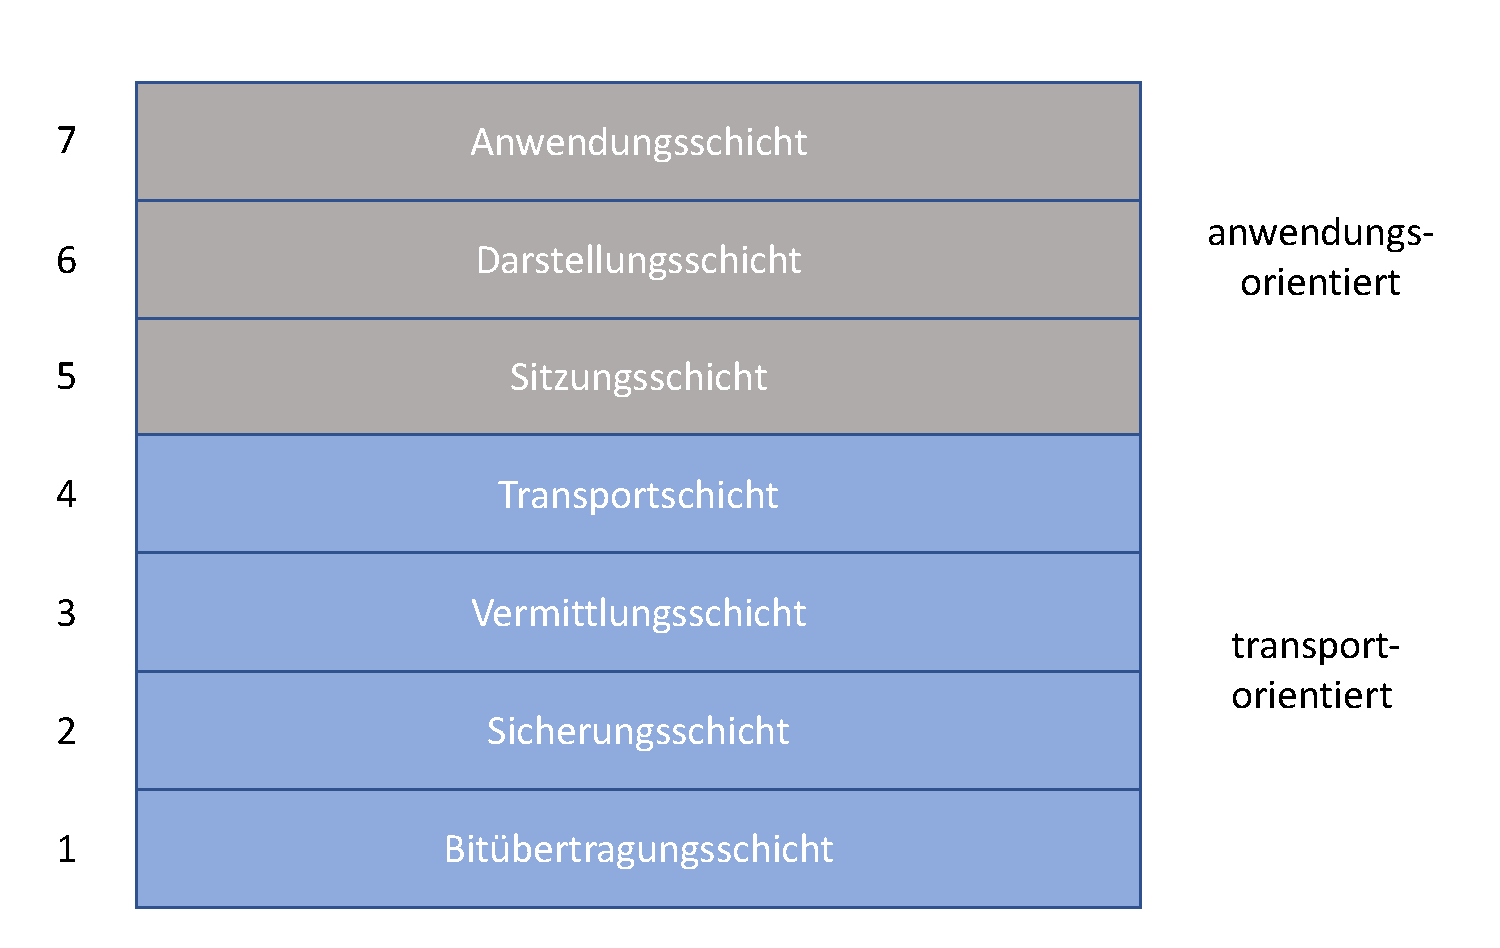
\includegraphics[width=0.6\linewidth]{gfx/OSI}} 
        \caption[OSI Referenzmodell]{\gls{osi}-Referenzmodell}\label{fig:osi}
\end{figure}
\begin{description}
\item[Layer 1:] Umwandlung der Bits in ein für den jeweiligen Übertragungskanal geeignetes Signal.
\item[Layer 2:] Gewährleistung einer fehlerfreien Übertragung und Regelung des Kanalzugriffs.
\item[Layer 3:] Ermittlung eines geeigneten Weges über mehrere Netzwerkknoten (\gls{routing}).
\item[Layer 4:] Zuordnung von Daten zu verschiedenen Anwendungen, welche dieselbe Verbindung nutzen, wie \zB E-Mail Client und Webbrowser.
\item[Layer 5-7:] Diese Schichten werden üblicherweise von dem Anwendungsprogramm zusammenhängend abgedeckt. Sie sind nicht mehr direkt auf die Datenübertragung bezogen, sondern beschreiben die Funktionalität der eigentlichen Anwendung.
\end{description}

Es ist zu ergänzen, dass die Sicherungsschicht im Unterschied zum ursprünglichen \gls{osi}-Modell in einigen Bereichen in zwei Unterschichten aufgeteilt wird. Dies ist der Fall, wenn Protokolle notwendig sind, die explizit den Kanalzugriff regeln. Die untere Teilschicht dient dann der \acf{mac}, während die obere Schicht eine Schnittstelle zur darüber liegenden Vermittlungsschicht beschreibt. Diese wird als \acf{llc}-Schicht bezeichnet.  

Bei Übertragungen wird der Protokollstapel beim Sender von oben nach unten durchlaufen. Dabei fügen die Protokolle der einzelnen Schichten jeweils Informationen zur eigentlichen Nachricht hinzu, bis hin zur Übertragung des Signals über ein physikalisches Medium, \zB ein Kabel oder Funkwellen. Am Empfänger durchläuft das Signal den Protokollstapel dann in umgekehrter Reihenfolge von unten nach oben. Dabei entfernen die Protokolle die jeweils zuvor hinzugefügten Informationen und nutzen diese zur Erfüllung ihrer Aufgaben, bis die ursprüngliche Nachricht in der Anwendung des Empfängers angekommen ist. Dazu definieren die einzelnen Schichten Schnittstellen --- sogenannte \acfp{sap}. Über diese Schnittstellen kommunizieren die Schichten mit Hilfe der vier folgenden Dienst-Primitiven:
\begin{itemize}
\item \texttt{REQ}: \emph{Request}, auf Deutsch \gqq{Anforderung}
\item \texttt{IND}: \emph{Indication}, auf Deutsch \gqq{Meldung}
\item \texttt{RESP}: \emph{Response}, auf Deutsch \gqq{Antwort}
\item \texttt{CONF}: \emph{Confirmation}, auf Deutsch \gqq{Bestätigung}
\end{itemize}
\begin{figure}[bth]
        \myfloatalign
        {
\includegraphics[width=0.4\linewidth]{gfx/Muster}} 
        \caption[Dienstprimitiven]{Struktur der Protokollschichten des \gls{802154} Standard}\label{fig:primitiven}
\end{figure}
\autoref{fig:primitiven} veranschaulicht  die Art und Weise, wie diese Primitiven eingesetzt werden. Mit \texttt{REQ} fordert Schicht $N$ einen Dienst der darunter liegenden Schicht $N-1$ an. Nach der Bearbeitung in Schicht $N-1$ antwortet diese mit \texttt{CONF}. Andersherum wird eine \texttt{IND} immer von der tieferen Schicht $N-1$ ausgelöst, um die höherliegende Schicht $N$ über ein Ereignis zu informieren. In diesem Fall antwortet $N$ mit \texttt{RESP}. Durchläuft beispielsweise eine Nachricht beim Empfänger den Protokollstapel, wie oben beschrieben, informieren die einzelnen Protokollschichten nach der Verarbeitung der Nachricht die nächst höhere Schicht durch eine \texttt{IND} Primitive.
Neben den eigentlichen Nutzdaten ist es auch möglich, dass protokolleigene Kommandos über das Medium übertragen werden. Dies ist der Fall, wenn eine Protokollinstanz des einen Gerätes Informationen mit der entsprechenden Protokollinstanz eines anderen Gerätes austauschen muss. Ein Beispiel dafür ist die Anforderung und Zuweisung einer Geräteadresse. Diese Kommandos werden wie gewöhnliche Nutzdaten vom Sender auch an die darunterliegenden Schichten weitergeleitet und über das Medium übertragen. Empfängerseitig durchlaufen sie den Stapel allerdings nur bis zum entsprechenden Protokoll. Auf diese Art werden die vielseitigen Herausforderungen einer erfolgreichen Kommunikation aufgeteilt. 

\subsection{Der IEEE 802.15.4 Standard}\label{kap:grundlagen_sec:802154}
\begin{figure}[bth]
        \myfloatalign
        {
\includegraphics[width=0.8\linewidth]{gfx/Muster}} 
        \caption[802.15.4 Protokollstapel]{802.15.4 Protokollstapel. Der Standard definiert die physikalische Schicht sowie die Kanalzugriffschicht. Eingezeichnet sind auch die Schnittstellen (\acsp{sap}) zum Datenaustausch zwischen den  Schichten.}\label{fig:802154_stack}
\end{figure}

Der \gls{802154} Standard ist ein Protokollstapel für drahtlose Netzwerke mit geringer Datenrate. \acsp{wsn} sind ein klassisches Beispiel solcher Netze. \gls{802154} definiert die physikalische Schicht --- den \emph{PHY Layer} --- sowie den unteren Teil der Sicherungsschicht --- den \emph{MAC Layer}. Die beiden Schichten übernehmen dabei die folgenden Aufgaben: 
\paragraph{MAC Layer}
Hier geschieht die notwendige Organistation der Nutzdaten. Es wird eine Rahmenstruktur definiert, in der die Nutzdaten zusammen mit Steuerinformationen untergebracht werden. Z.B werden die Nachrichten mit einer Sequenznummer versehen, um ggf. Empfangsbestätigungen zuordnen zu können. Weiterhin ermöglicht das Hinzufügen einer Prüfsumme eine Bitfehlererkennung. Der \emph{MAC Layer} bietet weiterhin die Möglichkeit, periodische Funksignale --- sogenannte \emph{Beacons} --- zu erzeugen, um Netzwerkteilnehmern regelmäßig organisatorische Informationen im Netzwerk bereitzustellen und eine Synchronisation der Teilnehmer zu ermöglichen. Der Standard sieht vor, dass es einen koordinierenden Funknoten im Netzwerk gibt --- den \acs{pan}-\emph{Coordinator}. Dieser kann mithilfe der \emph{Beacons} dann \zB festlegen, dass eine Kommunikation nur innerhalb eines definierten Zeitfensters stattfinden darf und sich daran eine Funkpause anschließt, in der alle Teilnehmer in einen energiesparenden passiven Modus wechseln können. Das Fenster, in dem die Kommunikation stattfindet, wird als \acf{cap} bezeichnet. Dazu wird ein \acs{csma} Algorithmus definiert (vgl. \autoref{kap:grundlagen_sec:kanalausnutzung}) \citep{ieee}.
\paragraph{PHY Layer}
Die Aufgabe der physikalischen Schicht im \gls{802154} Standard ist die Ansteuerung des \glspl{transceiver}. Dazu gehört die Wahl eines geeigneten Frequenzkanals und die Übertragung der einzelnen Bits unter Berücksichtigung der vom \gls{transceiver} bereitgestellten Modulationsverfahren (vgl. \autoref{kap:grundlagen_sec:modulation}). Daneben stellt der \emph{PHY Layer} Dienste zur Bewertung des Funkkanal zur Verfügung (\acs{cca}). Dieser Dienst wird vom darüber liegenden \emph{MAC Layer} während des \acs{csma} Algorithmus angefordert. Eine genaue Beschreibung dies Verfahrens erfolgt in \autoref{kap:zugriffsverfahren_sec:csma}.

Die Struktur des \gls{802154} Protokollstapels ist in \autoref{fig:802154_stack} dargestellt. Dort sind auch die \acsp{sap} eingezeichnet. Die Nutzdaten werden dabei über den \acf{mcps-sap} und den \acf{pd-sap} weitergeleitet. Steuerinformationen und Dienstanfragen werden dagegen über den \acf{mlme-sap} und den \acf{plme-sap} ausgetauscht.



\section{Energieverbrauch}\label{kap:grundlagen_sec:energieverbrauch}
Einleitend sei hier eine Anmerkung zum Begriff \gq{Energieverbrauch}  angeführt: Energie wird im eigentlichen Sinne nicht verbraucht, sondern umgewandelt - \zB von mechanischer Energie in elektrische Energie oder von elektrischer Energie in Strahlungsenergie. Dabei wird ein Teil der Energie immer in Wärme umgewandelt, die in der Regel nicht weiter genutzt werden kann. Mit \gq{Energieverbrauch} ist im Folgenden stets der Bedarf an elektrischer Energie  $E_\textrm{el}$ gemeint, der für die Funktion des Systems, speziell des \glspl{transceiver}, notwendig ist. 

Energie ergibt sich aus der Leistungsaufnahme über die Zeit:
\begin{equation}
{E =  P \cdot t}
\label{eq:energie}
\end{equation}
Die elektrische Leistung $P_\textrm{el}$ ist definiert als Produkt von Spannung und Strom:
\begin{equation}
{P_\textrm{el} =  U \cdot I}
\label{eq:leistung}
\end{equation}

Die SI-Einheit der Leistung ist \emph{Watt}, Sendeleistungen werden oft auch als logarithmisches Maß, bezogen auf ein \emph{Milliwatt}, in \emph{dBm} angegeben. Die SI-Einheit der Energie ist \emph{Joule} ($J$), die elektrische Energie wird üblicherweise auch in \emph{Wattsekunden} ($Ws$) bzw. \emph{Milliwattsekuden} ($mWs$) angegeben.
\begin{equation}
{1mWs = 0,001Ws = 0,001J}
\label{eq:Joule}
\end{equation}

Bei Funksystemen ist der \gls{transceiver} die relevante Komponente für den Energieverbrauch. Dieser ist für das Senden und Empfangen der Nachrichten zuständig. Wie in \autoref{kap:grundlagen_sec:wellenausbreitung} beschrieben, ist für eine erfolgreiche Funkübertragung eine ausreichend hohe Sendeleistung notwendig, aber auch die Verstärkung und Aufbereitung des schwachen Empfangssignals ist mit einer hohen Leistungsaufnahme verbunden. 
\begin{table}
    \myfloatalign
  \begin{tabularx}{\textwidth}{Xll} \toprule
    \tableheadline{Modus} & \tableheadline{Stromaufnahme} & \tableheadline{Leistungsaufnahme}\\ \midrule
    Power Down & $0,0005mA$ & $0,0015mW$ \\
    IDLE & $1,5mA$ & $4,5mW$ \\
    TX mit $14dBm$ & $46,0mA$ & $138mW$ \\
    TX mit $10dBm$ & $36,0mA$ & $108mW$ \\
    RX & $23,5mA$ & $70mW$ \\
    \bottomrule
  \end{tabularx}
  \caption[Leistungsaufnahme]{Nennwerte der Leistungsaufnahme des CC1200 Funkchips von Texas Instruments bei einer Betriebsspannung von 3,0V und einer Sendefrequenz von 869,5MHz \citep{CC1200data}}  \label{tab:leistungsaufnahme}
\end{table}
In \autoref{tab:leistungsaufnahme} sind exemplarisch die Angaben zur Leistungsaufnahme des \texttt{CC1200} Funkchips von \emph{Texas Instruments} aufgelistet. Die Leistungsaufnahme im Sendemodus (TX) und Empfangsmodus (RX) ist um mehrere Zehnerpotenzen höher als in den inaktiven bzw. datenverarbeitenden Modi (Power Down, IDLE). 

\subsection{Energiemodell}\label{kap:grundlagen_sec:energiemodell}
Um den Energieverbrauch des \glspl{transceiver} während der Funkkommunikation zu erfassen, kann dieser mit einem Zustandsautomaten modelliert werden, wie in \autoref{fig:energiemodell} dargestellt.
\begin{figure}[bth]
        \myfloatalign
        {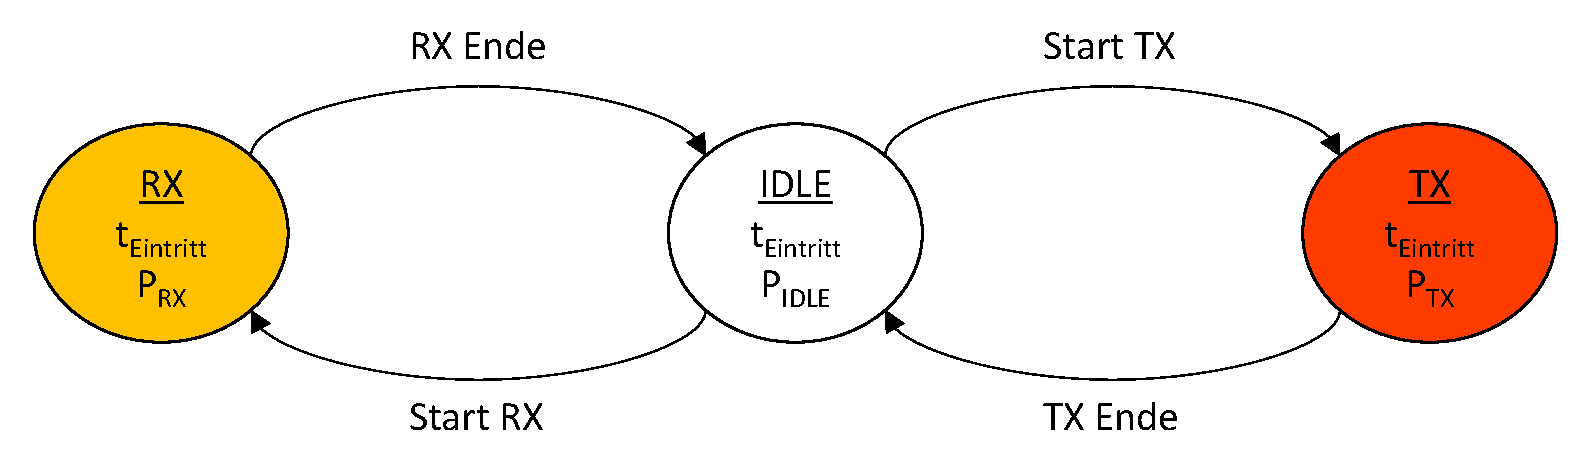
\includegraphics[width=1\linewidth]{gfx/Energiemodell}} 
        \caption[Energiemodell]{Zustandsmodell eines \glspl{transceiver} mit drei Betriebsmodi zur Erfassung des Enerievergrauchs}\label{fig:energiemodell}
\end{figure}
Zu den einzelnen Modi ist jeweils die entsprechende Leistungsaufnahme im Modell hinterlegt. Der \gls{transceiver} startet im IDLE-Zustand, dabei wird $t_\textrm{Eintritt}$ auf Null gesetzt. Findet \zB nach fünf Sekunden der erste Sendevorgang statt, wird zum ersten Mal der Energieverbrauch bestimmt: $E = P_\textrm{IDLE} \cdot 5s$ (vgl. \autoref{eq:energie}) und das Modell wechselt in den TX-Zustand. Der Zeitpunkt des Zustandswechsels wird in $t_\textrm{Eintritt}$ gespeichert. Dauert der Sendevorgang beispielsweise zwei Sekunden, wird beim dann folgenden Zustandsübergang zu IDLE der Energieverbrauch aktualisiert: $E = E + P_\textrm{TX} \cdot 2s$. Bei allen weiteren Zustandsübergängen wird analog verfahren. Durch Hinzufügen weiterer Zustände, für \zB einen \emph{Power Down}- oder Einschwingmodus mit den jeweiligen Leistungsaufnahmen, kann das Modell beliebig verfeinert werden.

\subsection{Energiemessung}\label{kap:grundlagen_sec:energiemessung}
Um die tatsächliche Leistungsaufnahme des verwendeten \glspl{transceiver} zu bestimmen, wird der in diesem Abschnitt beschriebene Messaufbau verwendet. Die Leistungsaufnahme kann bei bekannter Betriebsspannung $U_\textrm{B}$ nach \autoref{eq:leistung} durch die Messung des Stroms ermittelt werden. Dazu wird hier das \emph{PowerScale} System verwendet, das eine Strommessung im $\mu A$ Bereich erlaubt. Dabei wird eine Messeinheit über eine Schnittstelle mit dem zugehörigem Computerprogramm verbunden, wie in \autoref{fig:mess-uebersicht} zu erkennen ist. Der verwendete \gls{transceiver} ist der \gls{cc1200} von \emph{Texas Instruments} (s. \autoref{kap:grundlagen_sec:cc1200}). Dieser wird ebenfalls über eine Schnittstelle mit einem Diagnoseprogramm auf dem Computer verbunden, um den Chip in den zu vermessenden Modus zu versetzen. Zum Vermessen der Leistungsaufnahme im TX-Modus kann hier die Einstellung der verschiedenen Sendeleistungen vorgenommen werden. Zur Messung der Leistungsaufnahme im RX-Modus ist in Ergänzung zu den Komponenten in \autoref{fig:mess-uebersicht}  ein weiterer \gls{cc1200} notwendig, um Funknachrichten zu erzeugen.

\begin{figure}[bth]
        \myfloatalign
        \subfloat[Messaufbau]
        {\label{fig:mess-uebersicht}%
         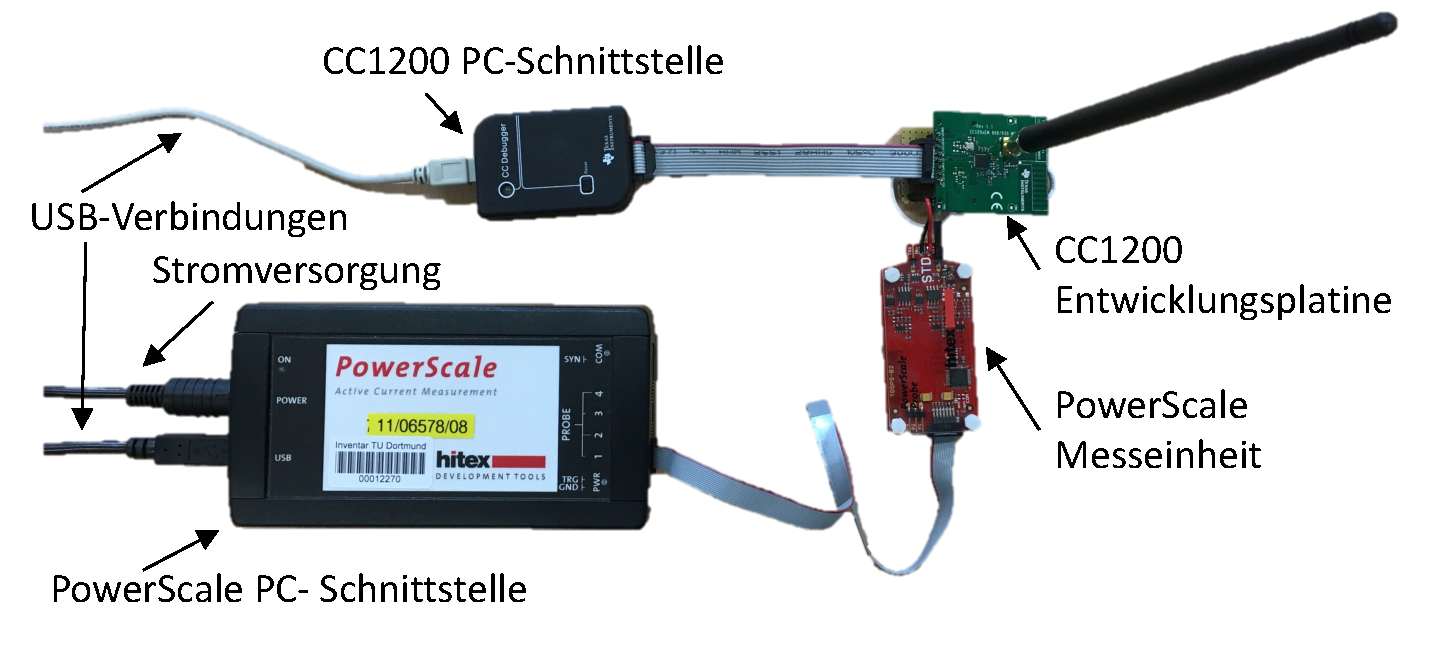
\includegraphics[width=1\linewidth]{gfx/Messuebersicht}} \\
        \subfloat[Messschema]
        {\label{fig:mess-schema}%
        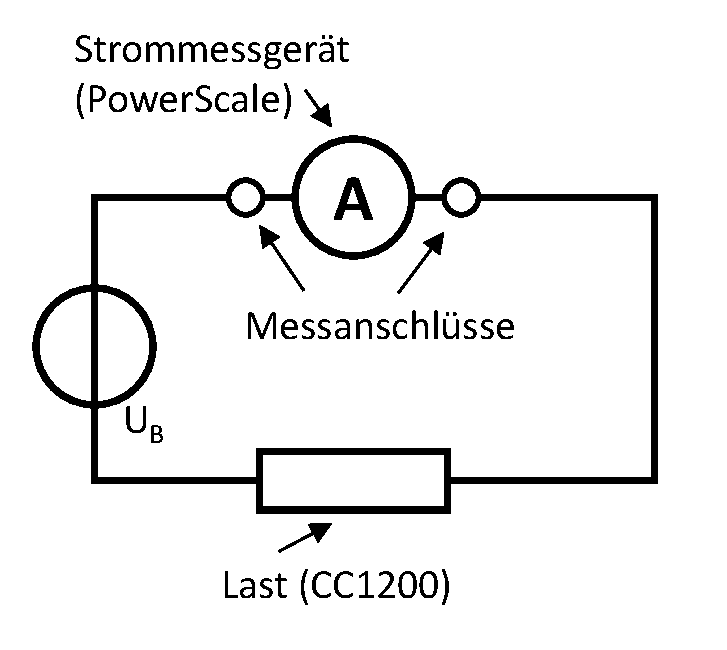
\includegraphics[width=0.4\linewidth]{gfx/Messschema}} 
        \subfloat[Detailansicht]
        {\label{fig:mess-detail}%
        \includegraphics[width=0.4\linewidth]{gfx/Messdetail}} 
        \caption[Energiemessung]{Aufbau zur Energiemessung des CC1200 \glspl{transceiver}}\label{fig:mess}
\end{figure}

Zur Messung des Stroms in einem elektrischen System muss das Strommessgerät in den Stromkreislauf integriert werden. Ein Schaltbild des Messaufbaus ist in \autoref{fig:mess-schema} dargestellt. Um diese Integration des PowerScale-Systems zu ermöglichen, ist ein Adapter notwendig, der die Stromzufuhr des gls{cc1200} unterbricht und die Anschlusspunkte für das Messsystem bereitstellt. \autoref{fig:mess-detail} zeigt den Anschluss im Detail. Durch die Verbindungen zur Messeinheit wird die Stromzufuhr zum Funkchip wieder geschlossen.

Das Messprogramm auf dem Computer speichert den Verlauf der momentanen Leistungsaufnahme. Im Anschluss kann der für den jeweiligen Betriebsmodus relevante Zeitbereich ausgewählt werden und das Programm berechnet den Energieverbrauch durch Aufsummierung der gemessenen Leistungswerte für den markierten Zeitraum.

\section{Simulationen}\label{kap:grundlagen_sec:simulation}

Simulationen können dann eingesetzt werden, wenn ein System zu komplex für eine konkrete Berechnung ist oder ein Versuchsaufbau unverhältnismäßig aufwendig wäre. Nachdem ein System in einem Simulationsmodell implementiert ist, liegt der Vorteil darin, schnell einen Überblick über die Auswirkungen verschiedener Parametervariationen zu erhalten. Nachteilig ist, dass ein Simulationsmodell in der Regel nicht alle Aspekte des realen Systems berücksichtigt. Je detailreicher das Modell sein muss, desto größer ist der Aufwand der Implementierung. 

Im Bezug auf Netzwerke liegt der Vorteil von Simulationen darin, dass an vielen Stellen des Netzwerkes, \zB an Empfängern in einem Sensornetzwerk, derselbe Prozess stattfindet. Dieser Prozess muss nur einmal formal beschrieben sein und kann in der Simulation dann immer wieder zu entsprechender Zeit durchlaufen werden. Ebenso ist eine Übersicht aller in der Simulation enthaltenen Größen zu jedem Zeitpunkt möglich. Ein weiterer Vorteil besteht in der exakten Reproduzierbarkeit der Untersuchung.
\subsection{Ereignisorientierte Simulation}
Bei \acfp{des} werden die zu bearbeitenden Ereignisse $($engl. \emph{Events}$)$ in eine Liste, die so genannte \acf{fel}, eingeordnet und gemäß ihrer zeitlichen Abfolge bearbeitet. Ein einfaches Beispiel für eine \acs{des} ist der Kassiervorgang an der Supermarktkasse, wie in \autoref{fig:kasse} angedeutet. Eine entsprechende Simulation könnte ein Modell der einkaufenden Personen, ein Modell der Kasse und ein Modell der Warteschlange beinhalten. Wenn das Personenmodell die Menge an eingekauften Artikeln enthält, das Modell der Kasse die Bearbeitungszeit in Abhängigkeit der Artikelanzahl und das Modell der Schlange die Zahl der wartenden Personen verwaltet, läuft die Simulation wie folgt ab: Das Simulationsprogramm kann nach einer geeigneten Zufallsverteilung \gqq{Anstellen-\emph{Events}} erzeugen. Ist die Warteschlange leer, wird von dem Modell der Warteschlange direkt ein \gqq{Kassieren-\emph{Event}} erzeugt. Dadurch wird das Modell der Kasse aufgerufen, das die Bearbeitungszeit berechnet und ein \gqq{Verlassen-\emph{Event}} an entsprechender Stelle in die \acs{fel} einfügt.
Der Vorteil besteht darin, dass die Simulation nur die einzelnen \emph{Events} berechnen muss, die Zeit dazwischen wird nicht simuliert. Mit diesem Beispiel kann dann \zB die durchschnittliche Länge der Warteschlange in Abhängigkeit von der Menge der eingekauften Artikel berechnet werden.

\begin{figure}[bth]
        \myfloatalign
        {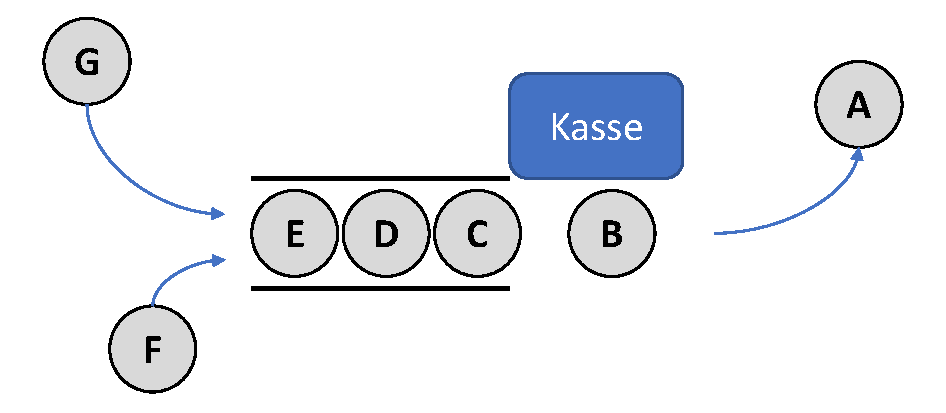
\includegraphics[width=0.6\linewidth]{gfx/kasse}} 
        \caption[Kasse]{angedeuteter Kassiervorgang als Beispiel für eine ereignisorientierte Simulation}\label{fig:kasse}
\end{figure}

Betrachtet man das genannte Beispiel aus einer abstrakten Sicht, so handelt es sich um ein System, bei dem eine Instanz, hier die Kasse, nach einer festgelegten Art eingehende Aufträge abarbeiten muss. Dieses Muster liegt auch den Vorgängen in Kommunikationsnetzen zugrunde, daher eignet sich eine \acl{des} besonders gut zur Unterschung von Netzwerken.

\subsection{OMNeT++}\label{kap:grundlagen_sec:omnet}
\gls{omnet} ist ein Simulationsframework für \acsp{des}, bei dem die Modellierung der einzelnen Komponenten in der Programmiersprache \gls{cpp} erfolgt. Wesentliche Aufgabe des Frameworks ist die Verwaltung der \acs{fel} und der Aufruf des Programmcodes der einzelnen Komponenten. \gls{omnet} bietet zusätzlich eine eigene Programmiersprache --- die \emph{NED}-Sprache --- an. Mit dieser können Gruppierung, Anordnung und Verbindungen der einzelnen Komponenten beschrieben werden.
Die wichtigsten Bestandteile von \acs{omnet} sind:
\begin{description}
\item[Module] Die einzelnen Komponenten der Simulation werden Module genannt. Mit der \gls{cpp}-Klasse \texttt{cModule} stellt das Framework eine Basisklasse zur Implementierung bereit. Während die Implementierung in \gls{cpp} erfolgt, wird die gegenseitige Beziehung zwischen verschiedenen Modulen in \emph{NED} beschrieben. Module können ineinander verschachtelt werden und besitzen Verbindungen zu anderen Modulen.

\item[Gates] Um \emph{Events} an andere Module zu senden, besitzen Module \emph{Gates}. Diese sind die eindeutigen Endpunkte einer Verbindung zwischen zwei Modulen. Schickt ein Modul ein \emph{Event} an ein \emph{Gate}, wird es genau dem Modul zugestellt, welches mittels der \emph{NED}-Sprache damit verknüpft ist. Module können mehrere \emph{Gates} besitzen. Außerdem können \emph{Events} direkt an ein \emph{Gate} eines anderen Moduls geschickt werden, ohne eine zuvor festgelegte Verbindung. Dies ist \zB für große Netzwerke mit variabler Anzahl an Teilnehmern sinnvoll. 

\item[Messages] \emph{Events} werden in \gls{omnet} \emph{Messages}, auf Deutsch \gqq{Nachrichten}, genannt. Im Zusammenhang mit Netzwerksimulationen ist anzumerken, dass dabei nicht zwangsläufig Nachrichten im Sinne des Netzwerkes gemeint sind, sondern dass es sich hierbei um jegliche Art von \emph{Event} in der Simulation handeln kann, \zB ein \emph{Timer-Event}.
\end{description}

\section{Hardware}\label{kap:grundlagen_sec:hardware}
In diesem Kapitel werden die Hardwarekomponenten vorgestellt, die zur prototypischen Implementierung des Systems verwendet werden. Die für die Funkkommunikation zentrale Komponente ist der CC1200 Funkchip von Texas Instruments. Für die Implementierung des Kanalzugriffprotokolls und zur Ansteuerung des Funkchips kommt der MSP430FR9596 Mikrocontroller von Texas Instruments zum Einsatz. Für beide Chips steht eine Entwicklungsplatine zur Verfügung.
\begin{figure}[bth]
        \myfloatalign
        \subfloat[MSP430 LaunchPad]
        {\label{fig:platinen-msp}%
        \includegraphics[width=0.5\linewidth]{gfx/MSP_Board}} 
        \subfloat[CC1200 EM]
        {\label{fig:platinen-cc1200}%
        \includegraphics[width=0.5\linewidth]{gfx/CC1200_Board}} 
        \caption[Entwicklungsplatinen]{Entwicklungsplatinen für Mikrokontroller und \gls{transceiver} zur prototypischen Anwendungsimplementierung}\label{fig:platinen}
\end{figure}
Entwicklungsplatinen vereinfachen die Entwicklung von Anwendungen, indem sie die nötige Beschaltung der Chips mit zusätzlichen Bauelementen realisieren und wichtige Schnittstellen zur Verfügung stellen. \autoref{fig:platinen-msp} zeigt das MSP430 \emph{LaunchPad}. Dieses verfügt neben zwei \acsp{led} und zwei Tastern über Elektronik zur Programmierung des Mikrocontrollers per USB Verbindung. Daneben sind einige der \acs{gpio}-Pins zur einfachen Verdrahtung an Stiftleisten herausgeführt. In \autoref{fig:platinen-cc1200} ist die CC120x EM Platine zu sehen. Darauf ist der CC1200 Funkchip mit den entsprechenden externen Kondensatoren und Widerständen versehen, die für exakte Frequenzerzeugung notwendig sind. Weiterhin ist ein coaxialer Antennenanschluss vorhanden. An der Stiftleiste auf der linken Seite befinden sich die Signalleitungen zur Ansteuerung des Funkchips.

Die folgenden Abschnitte beschreiben die beiden Hardwarekomponenten im Detail und geben wichtige Hinweise für die Implementierung.

\subsection{MSP430}\label{kap:grundlagen_sec:msp430}
Mikrocontroller vereinen einen Prozessor (\acs{cpu}), Speicher und weitere Peripherie, wie Timer, acf{adc} und serielle Kommunikation in einem Chip. Die einzelnen Pins des Mikrocontrollers können zur Ansteuerung von Aktoren oder zum Auslesen von Sensoren genutzt werden. Die Pins werden als \acf{gpio}-Pins bezeichnet. Die Mikrocontroller der MSP430 Reihe sind darüber hinaus speziell für Anwendungen mit begrenzten Energieressourcen konzipiert. \autoref{tab:msp} zeigt die Hauptmerkmale des verwendeten Modells.

\begin{table}
    \myfloatalign
  \begin{tabularx}{0.7\textwidth}{Xll} \toprule
    %\tableheadline{Modus} & \tableheadline{Stromaufnahme} & \tableheadline{Leistungsaufnahme}\\ \midrule
    Modell & MSP430FR9596 \\
    Hersteller & Texas Instruments \\
    Betriebsspannung & 1,8V - 3,6V \\
    Architektur & 16 Bit \gls{risc} \\
    Taktrate & 32kHz - 24MHz \\
    Speicher & 64kB \acs{fram} \\
    \bottomrule
  \end{tabularx}
  \caption[MSP Merkmale]{Eigenschaften des MSP430 Mikrocontrollers \citep{MSPdata}}  \label{tab:msp}
\end{table} 

Die Programmierung erfolgt üblicherweise in der Programmiersprache \gls{c}. Für die Konfiguration und Ansteuerung der einzelnen Peripheriekomponenten sind spezielle Register im Speicher des Mikrocontrollers vorgesehen. Obwohl sie sich für das Programm wie normale Speicheradressen verhalten und auch so beschrieben oder gelesen werden können, steuern die Bits dieser Register das Verhalten der integrierten Peripherie. So bestimmt beispielsweise der Wert in einem \acs{gpio}-Register die Spannungspegel der Pins am entsprechenden Port. Andersherum kann aus Registern, die dem \acs{adc} zugeordnet sind, das Ergebnis der Analog-Digital Wandlung entnommen werden. Da auf Mikrocontrollern in vielen Fällen kein Betriebssystem läuft, das einzelne Programmstarts verwaltet, wird ein Programm für Mikrocontroller als Endlosschleife programmiert, wie in \autoref{lst:while} angedeutet.
\begin{lstlisting}[float=h,language=C,frame=tb,captionpos=b,caption={Strukturbeispiel eines Programms für Mikrocontroller},label=lst:while]
// Code, der zu Beginn einmal durchlaufen wird
// zB. Konfigurationen der Peripherie

while(1) {
	// hier erfolgt die Implementierung der Anwendung
}

// Programmende wird nie erreicht
\end{lstlisting}

Da die Entwicklung des Programms nicht auf dem Mikrocontroller selbst stattfindet, wird eine Software benötigt, die das \gls{c}-Programm für die Verwendung auf dem Chip kompiliert. Im Anschluss wird der Quellcode mit einem \emph{Programmer} auf den Chip übertragen. Auf dem \emph{LaunchPad} ist dieser, wie eingangs erwähnt, bereits vorhanden.

Für die Realisierung von Anwendungen mit geringer Leistungsaufnahme kann der MSP430 in sieben unterschiedliche Energiesparmodi versetzt werden, bei denen stufenweise einzelne Komponenten und Taktquellen abgeschaltet werden. Bei der 	Rückkehr aus den Modi 3.5 und 4.5 bleiben alle Pins des Controllers durch das Kontrollbit \texttt{LOCKLPM5} im \texttt{PM5CTL0} Register gesperrt, um zunächst alle Konfigurationen vorzunehmen und die Pins anschließend freizugeben. Dieser Zustand tritt auch nach jedem Systemstart ein. Um die Pins des MSP430 nutzen zu können, muss dieses Bit zu beginn des Programms auf Null gesetzt werden.

Eine weitere Besonderheit beim MSP430 ist, dass der \gls{watchdog}-\emph{Timer} standardmäßig aktiviert ist. Ein \gls{watchdog}-\emph{Timer} ist ein Zähler, der unabhängig von der \acs{cpu} hardwareseitig in einigen Mikrocontrollern integriert ist und bei Erreichen eines eingestellten Wertes einen Neustart des Systems auslöst, so er nicht regelmäßig vor seinem Ablauf durch die Software zurückgesetzt wird. Diese Technik dient dem automatischen Neustart des Controllers, für den Fall eines unerwarteten Fehlverhaltens. Es ist beim MSP430 daher darauf zu achten, den \gls{watchdog}-Timer entsprechend regelmäßig zurückzusetzen oder ganz zu deaktivieren.

Drei für die Programmierung des Funkchips und die Implementierung des Kanalzugriffverfahrens wichtige Komponenten sind die Interrupt-Behandlung, die Verwendung von \emph{Timern} und die \gls{gl:spi} Kommunikation.

\paragraph{Interrupts}
Um auf Ereignisse Ereignisse, wie das eintreffen eines Bytes über die serielle Schnittstelle, die Änderung des Spannungspegels an einem Pin oder den Ablauf eines \emph{Timers} reagieren zu können, kann der normale Programmablauf durch einen Interrupt unterbrochen werden. Tritt ein Interrupt ein, wird zunächst das zugehörige Interrupt /emph{Flag} zur Signalisierung gesetzt. Ist der jeweilige Interrupt softwareseitig aktiviert, beginnt der Mikrocontroller mit der Abarbeitung einer separaten Programmsequenz - der \acf{isr}. Die Startadresse dieses Programmabschnitts ist in der Interruptvektor Tabelle gespeichert. Der MSP430 verfügt über 26 verschiedene Interruptvektoren, die zum Großteil den Peripheriekomponenten zugeordnet sind. Einigen Komponenten sind auch zwei Vektoren zugeordnet. So können individuelle Behandlungsroutinen (\acsp{isr}) geschrieben werden, ohne erst die Quelle des Interrupts ermitteln zu müssen. Dies führt zu einer schnelleren Behandlung des Ereignisses. Ist die \acl{isr} abgearbeitet, wird mit dem normalen Programmablauf fortgefahren. 

Bei der Verwendung von Interrupts ist darauf zu achten, dass es nicht zu unkontrollierten Manipulationen von gemeinsam genutzten Daten kommt. Durchläuft das Hauptprogramm \zB ein Array, in dem die Daten der letzten seriellen Übertragung gespeichert sind, muss sicher gestellt werden, dass diese Daten bis zum Ende des Durchlaufs nicht von einer \acs{isr} überschrieben werden.

\paragraph{Timer}
Der Grundbaustein eines \emph{Timers} ist ein Zählregister, dessen Wert in definierten Abständen inkrementiert wird. Diese Abstände hängen mit dem Systemtakt zusammen. Die Taktrate des Zählers lässt sich über Vorteiler bezogen auf die Systemtaktrate einstellen. Durch diese Einstellung wird die minimal zu messende Zeit des \emph{Timers} festgelegt. Die Größe des Zählregisters bestimmt die Auflösung des \emph{Timers}, also die Anzahl von Schritten bis zum Erreichen des Höchstwertes und damit zum Ablauf \emph{Timers}. Die Funktionsweise ist in \autoref{fig:timer} für eine Auflösung von vier Bit, also acht Zählwerten, verdeutlicht. Die Auflösung beim MSP430 beträgt 16 Bit.
\begin{figure}[bth]
        \myfloatalign
        {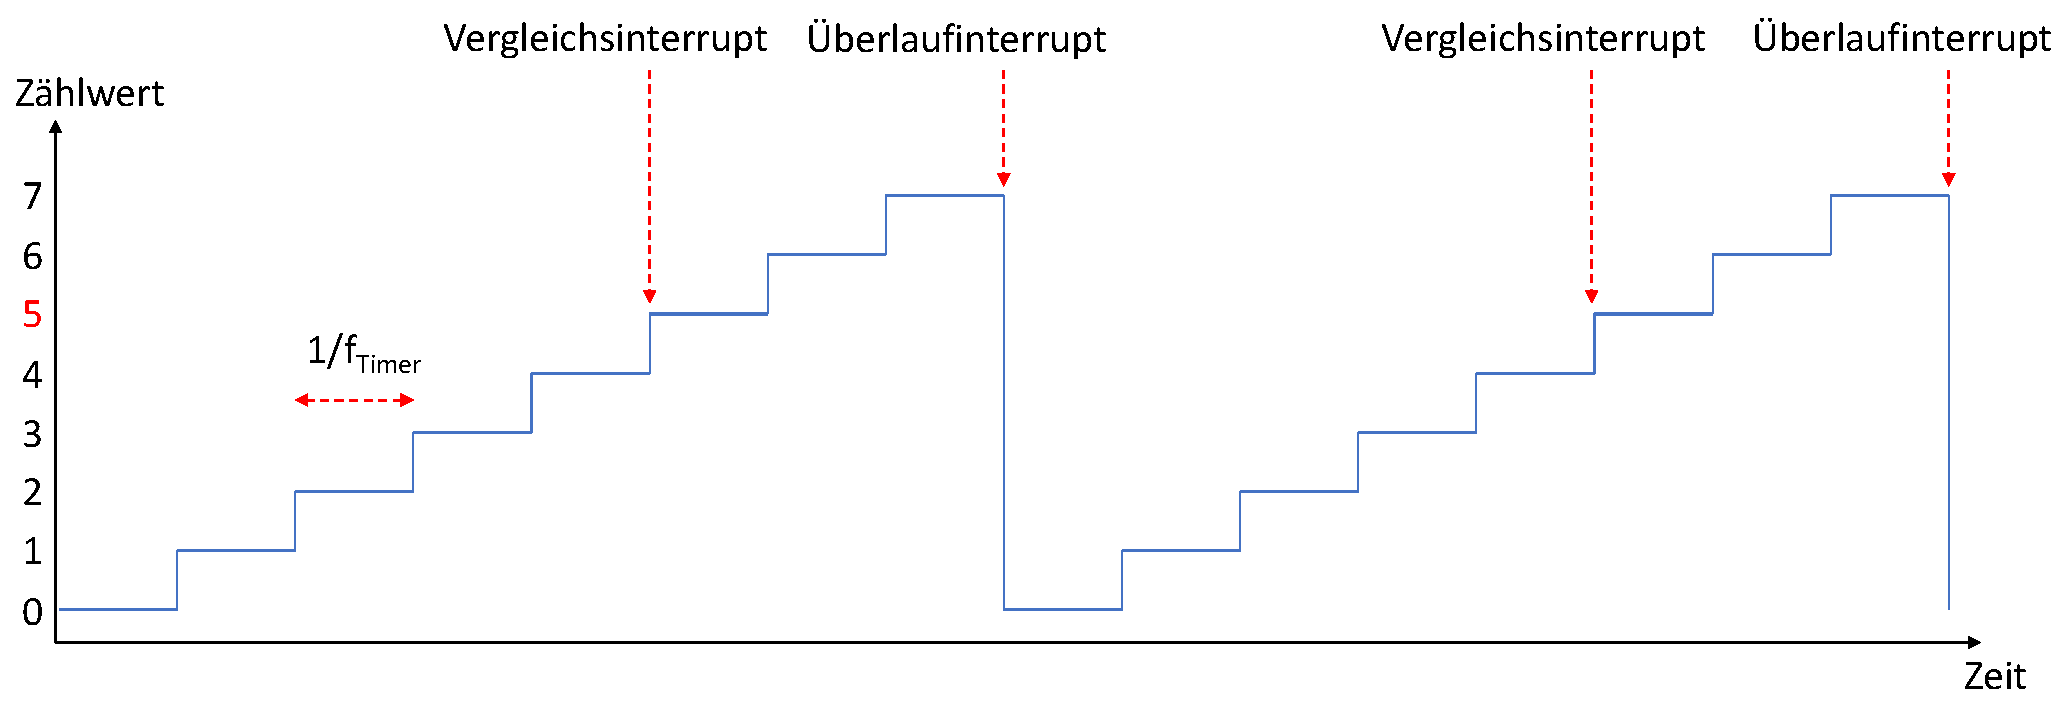
\includegraphics[width=\linewidth]{gfx/Timer}} 
        \caption[Timer]{Funktionsweise eines 4-Bit \emph{Timers}. Der rotmarkierte Wert kennzeichnet den eingestellten Vergleichswert.}\label{fig:timer}
\end{figure}
Da die Einstellung der Taktrate $f_\textrm{Timer}$ nur in bestimmten Schritten möglich ist, bietet der MSP430 zusätzlich die Möglichkeit, einen Interrupt auszulösen, wenn ein definierter Vergleichswert erreicht wird, in \autoref{fig:timer} in rot markiert. Dieser Wert kann über ein Register eingestellt werden und erlaubt so ein sehr feine Einstellung des Interruptzeitpunkts.

\paragraph{SPI}
Das \acf{spi} des Mikrocontroller bietet die Möglichkeit eine synchrone serielle Buskommunikation mit Peripheriegeräten, wie \zB dem CC1200 Funkchip, herzustellen. Die Kommunikation wir dabei stets von einem Gerät initialisiert, dem \emph{Master}. Die angeschlossenen Geräte werden als \emph{Slaves} bezeichnet. Dazu werden drei gemeinsame Signalleitungen benötigt und zusätzlich eine Leitung pro \emph{Slave}:
\begin{enumerate}
\item \gls{gl:mosi}
\item \gls{gl:miso}
\item \gls{gl:scl}
\item \gls{gl:cs}
\end{enumerate}

Zu Beginn der Kommunikation muss der \emph{Master} die beteiligten Kommunikationspartner aktivieren, dies geschieht über die \gls{gl:cs}, engl. \acl{cs}.
Anschließend erzeugt der \emph{Master} auf der \gls{gl:scl} regelmäßige Signalflanken, engl. \acl{scl}. Mit dieser Frequenz wird dann der Pegel der \gls{gl:mosi} entsprechend der zu übertragen Bits auf Null oder Eins geändert, sodass der \emph{Slave} diese bei jeder Taktflanke abtasten kann, engl. \acl{mosi}. Gleichzeitig kann der \emph{Slave} über die \gls{gl:miso} Daten an den \emph{Master} in analoger Weise senden, engl. \acl{miso}.
Der MSP430 realisiert diese Bussystem in einer Hardwareeinheit zur seriellen Kommunikation. Nach entsprechender Konfiguration, kann ein zu sendendes Byte in dafür vorgesehenes Register geschrieben werden. Der Controller startet dann automatisch den Kommunikationsvorgang. Die übertragenen Daten des \emph{Slaves} werden ebenfalls in einem Register abgelegt und können ausgelesen werden. Nach vollständiger Übertragung kann ein Interrupt ausgelöst werden. Ein Mitschnitt der \gls{gl:spi} Kommunikation zwischen MSP430 und dem CC1200 Funkchip ist in \autoref{fig:spi} zu sehen.

\subsection{CC1200 Funkchip}\label{kap:grundlagen_sec:cc1200}
Der CC1200 Funkchip von Texas Instruments ist ein Transceiver für den Sub-GHz Bereich mit umfassenden Konfigurationsmöglichkeiten zur Sendefrequenz, Moduation (vgl. \autoref{kap:grundlagen_sec:modulation}), zur Paketverarbeitung und Kanalprüfung. Die wesentlichen Merkmale sind in \autoref{tab:cc1200} aufgelistet. Einen besonders sparsamen Betrieb erreicht der CC1200 durch den sogenannten \emph{Sniff}-Modus. \autoref{fig:sniff} veranschaulicht die Vorteile gegenüber dem normalen Empfangsmodus. Der \gls{transceiver} fügt vor den Nutzdaten eine Präambel und ein Synchronisationsbyte ein, um den Beginn der Nachricht zu markieren und die Empfangselektronik kalibrieren zu können. Der CC1200 ist in der Lage, den Beginn einer Nachricht nach vier Präambel-Bits zu detektieren. Des Weiteren benötigt der Chip nur ca. $0,6ms$, um vom Ruhemodus in den Empfangsmodus zu wechseln \citep{CC1200data}. Diese Eigenschaften erlauben es im \emph{Sniff}-Modus in regelmäßigen Abständen kurz in den Empfangsmodus (RX) zu schalten, während der Chip zum größten Teil im energiesparenden Ruhemodus verbleibt. Dazu muss die Präambellänge deutlich erhöht werden, um kein Paket zu verpassen, wie in \autoref{fig:sniff2} zu erkennen ist. Sie muss so groß sein, dass im dargestellten ungünstigsten Fall --- das Paket beginnt genau nachdem der Chip gerade in den Ruhemodus gewechsel ist --- noch mindestens vier Präambel-Bytes beim nächsten Wechsel zu RX detektiert werden können. Es ist noch anzumerken, dass dieses Verfahren nur für den Empfang von Paketen vorgesehen ist. Zum Zweck der Kanalüberprüfung ist der kontinuierliche RX-Modus nötig.

\begin{table}
    \myfloatalign
  \begin{tabularx}{\textwidth}{Xll} \toprule
    %\tableheadline{Modus} & \tableheadline{Stromaufnahme} & \tableheadline{Leistungsaufnahme}\\ \midrule
    Modell & CC1200 \\
    Hersteller & Texas Instruments \\
    Betriebsspannung & 3,3V \\
    primäre Frequenzen & 169MHz, 433MHz, 868MHz, 915MHz \\
    maximale Sendeleistung & 16dBm \\
    Empfindlichkeit & -109dBm bei 50kBits/s \\
    maximale Datenrate & 1,25MBits/s  \\
    Sende-/Empfangsspeicher & je 128 Byte  \\
    \bottomrule
  \end{tabularx}
  \caption[CC1200 Merkmale]{Eigenschaften des CC1200 Funkchips \citep{MSPdata}}  \label{tab:cc1200}
\end{table}

\begin{figure}[bth]
        \myfloatalign
        \subfloat[Normaler Empfangsmodus]
        {\label{fig:sniff1}%
        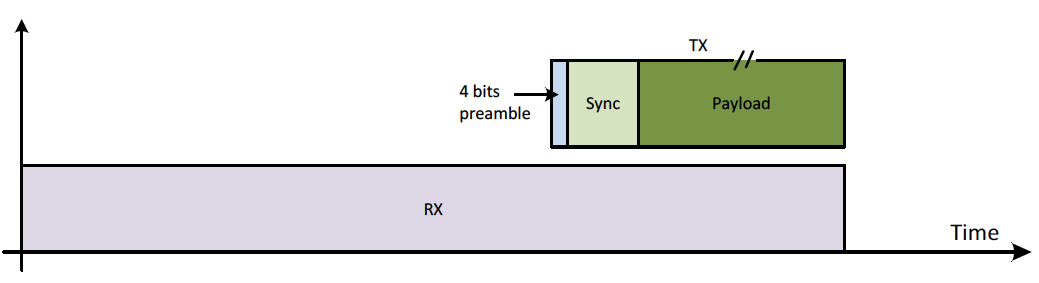
\includegraphics[width=\linewidth]{gfx/Sniff1}} \\
        \subfloat[Sniff Modus]
        {\label{fig:sniff2}%
        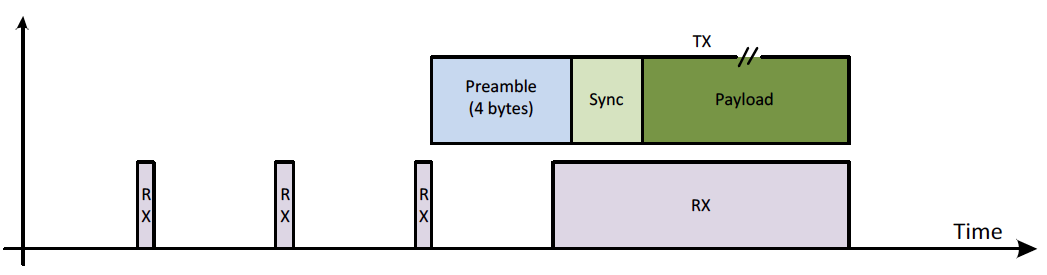
\includegraphics[width=\linewidth]{gfx/Sniff2}} 
        \caption[CC1200 Sniffmode]{Auszug aus dem CC1200 \emph{User's Guide} zur Veranschauichung des energiespareden \emph{Sniff}-Modus \citep{CC1200guide}}\label{fig:sniff}
\end{figure}

Die Ansteuerung des CC1200 Funkchips erfolgt über \gls{gl:spi}. Der Informationsaustausch zwischen Mikrocontroller und CC1200 lässt sich dazu in drei Rubriken einteilen:
\begin{enumerate}
\item Schreiben bzw. Lesen der insgesamt 209 Konfigurationsregister zur Einstellung der Sendefrequenz, Modulationsart, Paketlänge, etc..
\item Senden von Kommandos, den so genannten \emph{Strobes}, um den Funkchip in den gewünschten Modus zu versetzen.
\item Austausch von Sende- und Empfangsdaten.
\end{enumerate}

Die Art der Informationsübertragung wird durch das erste Byte bestimmt, welches der Mikrocontroller an den Funkchip sendet. Letzterer erwartet dann weitere Informationen in Form von Bytes in einem festgelegten Muster. Wird durch das erste Byte signalisiert, dass der Chip seinerseits Daten über den Bus senden soll, gilt dies analog. Für den Fall, dass keine Daten vom Chip angefordert werden, sendet dieser bei jeder Übertagung ein Statusbyte an den Mikrocontroller, aus dem der aktuelle Modus und etwaige Fehlermeldungen entnommen werden können. Diese individuellen Übertragungsmuster erfordern, dass die \gls{gl:cs} während des ersten Bytes und allen evtl. folgenden Bytes kontinuierlich durch den Mikrocontroller auf Null-Pegel gehalten wird. Dies ist bei Konfiguration des MSP430 zur automatischen \gls{gl:spi} Steuerung (vgl. \autoref{kap:grundlagen_sec:msp430}) nicht gegeben, da die \gls{gl:cs} dabei nach jedem Byte wieder deaktiviert wird. Um die Übertragung nicht abzubrechen, muss der Pin für die \gls{gl:cs} separat durch die Software angesteuert werden. Beispielhaft ist in \autoref{fig:spi} der Schreibvorgang in ein Konfigurationsregister des CC1200 zu sehen, das sich im erweiterten Adressraum befindet. In diesem Fall signalisiert das erste Byte lediglich, dass es sich um einen Zugriff auf den erweiterten Adressraum handelt. Der Funkchip erwartet dann die Adresse im zweiten übertragenen Byte und schließlich den Wert, der an diese Adresse geschrieben werden soll.


\begin{figure}[th]
        \myfloatalign
        {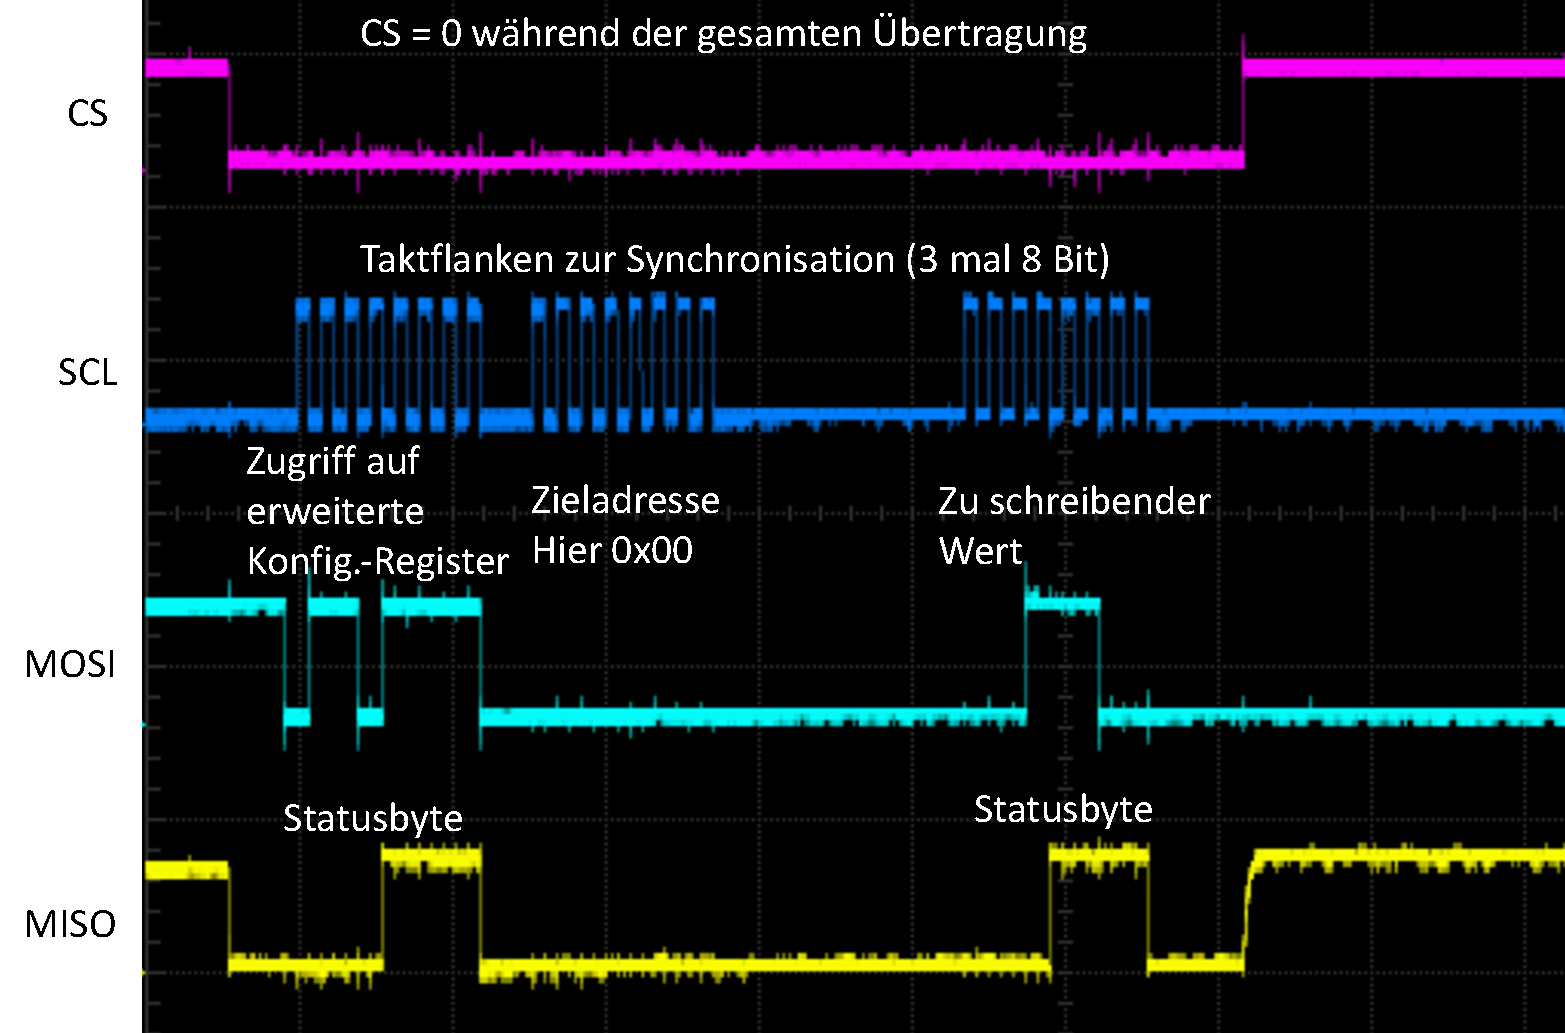
\includegraphics[width=\linewidth]{gfx/SPI}} 
        \caption[SPI]{Mitschnitt der SPI-Kommunikation zwischen MS430 und CC1200. Zu sehen ist der Schreibvorgang eines Konfigurationsregisters des CC1200 im erweiterten Adressraum.}\label{fig:spi}
\end{figure}

\section{Entwicklungssoftware}\label{kap:grundlagen_sec:software}

Neben der bereits in \autoref{kap:grundlagen_sec:omnet} beschriebenen Simulationsumgebung \gls{omnet} und dem in \autoref{kap:grundlagen_sec:energiemessung} vorgestellten \emph{PowerScale} Systems sind noch weitere Entwicklungs- und Diagnosewerkzeuge für diese Arbeit notwendig. Deren Aufgaben im Rahmen dieser Arbeit werden hier aufgeführt.

\begin{description}
\item[Code Composer Studio] Eine Entwicklungsumgebung zur Programmierung des MSP430 Mikrocontrollers. Neben der Verwaltung der einzelnen Quellcodedateien und der in \autoref{kap:grundlagen_sec:msp430} genannten Übersetzung des \gls{c}-Codes in Maschinenbefehle, bietet diese Software die Möglichkeit zum \emph{Debugging}, auf Deutsch \gqq{Fehlersuche}. Dabei kann der auf den Mikrocontroller geladene Programmcode schrittweise ausgeführt werden. Außerdem können die Registerwerte und Variablen ausgelesen werden. Die Möglichkeit des \emph{Debuggings} muss von der Hardware unterstützt werden. Das \emph{LaunchPad} bietet diese Möglichkeit.

\item[RF Studio / Packet Sniffer] Zwei Softwarewerkzeuge die über eine Hardwareschnittsstelle --- dem \emph{CC12xx Debugger} --- die Register des CC1200 Funkchips direkt schreiben und auslesen können. Zum einen kann der Funkchip so auch ohne Mikrocontroller konfiguriert und in Betrieb genommen werden, zum anderen ist es möglich, empfangene Daten auf dem Computer anzeigen zu lassen und einige Verarbeitungsinformationen des CC1200 auszulesen. Dazu gehören die Empfangsqualität, das Ergebnis der Bitfehlerprüfung sowie der Zeitstempel von empfangenen Nachrichten.

\item[hterm] Ein Terminalprogramm zur byteweisen seriellen Datenübertragung. Dieses wird benutzt, um Informationen mit dem Mikrocontroller auszutauschen. Dieser Informationsaustausch bezieht sich nicht auf die Programmierung des Controllers, sondern auf den Austausch von Daten aus dem laufenden Programm heraus. Dabei besteht die Möglichkeit, die Daten sowohl in Textform, als auch in binärer oder hexadezimaler Darstellung einzugeben und anzeigen zu lassen. 
\end{description}
%*****************************************
%*****************************************
%*****************************************
%*****************************************
%*****************************************





%************************************************
\chapter{Verwandte Arbeiten}\label{kap:verwandtearbeiten}
%************************************************

Die Untersuchung von \ac{wsn} und den damit verbundenen Fragestellungen ist Forschungsgegenstand auf vielen verschieden Gebieten. Dieses Kapitel gibt einen Überblick über verschiedene Anwendungsfelder sowie zu Untersuchungen spezieller Aspekte. Anschließend werden drei Projekte mit besonderer Relevanz für die vorliegende Arbeit genauer beschrieben.

\section{Übersicht}

Obwohl Simulationen zur Erforschung von \acp{wsn} wegen der großen Anzahl unterschiedlicher Einflüsse nur bedingt zu umfassenden Ergebnissen führen können, sind sie dennoch wichtiger, begleitender Bestandteil vieler Untersuchungen.
\begin{description}

\item[IEEE 802.15.4 Modell] Ein Modell für die Simulationsumgebung \acs{omnet} aus dem Jahr 2007 \citep{oldmodel}. Der Fokus dieser Implementierung liegt auf der Modellierung des \acs{csma} Algorithmus

\item[Standalone IEEE 802.15.4 Modell] Eine nahezu vollständige Modellierung des \gls{802154} Protokolls für \gls{gl:omnet} \cite{model}. Neben den eigentlichen Protokollschichten, ist die Einbindung einer Anwendungsschicht bereits vorgesehen. Die Implementierung berücksichtigt einige Neuerungen des Protokolls im Vergleich zum zuvor genannten Modell.

\item[Batteriemodell] Zur genaueren Abbildung der Batterielaufzeit energiesensitiver Geräte innerhalb eines Simulationsszenarios wird in \cite{batterymodel} ein Batteriemodell vorgestellt, welches die komplexen elektro-chemischen Vorgänge berücksichtigt.

\end{description}
Um den Einschränkungen und Vereinfachungen bei simulativen Untersuchungen von \acs{wsn} entgegen zu wirken, gibt es eine Vielzahl von Versuchsplattformen, so genannten \emph{Testbeds}. Dort können die zu untersuchenden Systeme unter Real- \bzw Laborbedingungen erprobt werden.
\begin{description}

\item[MoteLab] Dieser Versuchsaufbau wurde 2005 an der Universität von Harvard errichtet und ist eine der ersten und am längsten betriebenen Untersuchungsplattformen für Sensornetze \citep{survey}. Diese besteht aus 190 drahtlos verknüpften \glspl{node}. Dabei kommt die \gqq{MicaZ}-Hardwareplattform zum Einsatz. Diese unterstützt u.a. Licht-, Temperatur-, Luftdruck,- und Beschleunigungssensoren und nutzt das \gls{zigbee} Protokoll im $2,4GHz$ Band zur Kommunikation. Zusätzlich sind die \glspl{node} kabelgebunden mit einem zentralen Server verbunden. Dieser ermöglicht es, die \glspl{node} zu programmieren und Daten mitzuschreiben. Über eine Webschnittstelle können Benutzer auf das Testbed zugreifen und individuelle Anwendungen darauf testen \cite{Motelab}.

\item[Kansei] Diese Plattform setzt sich aus drei Testsystemen zusammen. Hauptbestandteil bildet ein statisches Netz mit 210 \glspl{node} in eimem Labor. Dazu kommt ein Satz an portablen Sensorknoten, der je nach Anwendungsfall zur Messgrößenerfassung an bestimmten Orten eingesetzt werden kann. Des Weiteren gibt es \glspl{node}, die an mobilen Robotern angebracht sind \cite{Kansei}. Die \glspl{node} sind neben Licht-, Temperatur- und Infrarotsensoren auch mit einem Magnetometer und einem Mikrofon ausgestattet. Die Kommunikation findet im $433MHz$ Band statt.

\item[WISEBED] Insgesamt 750 \glspl{node} sind Bestandteil dieses Testbeds. Dabei sind sie in mehrere Gruppen aufgeteilt, die sich an neun verschiedenen Orten in Europa befinden. Die Sensorhardware der einzelnen Gruppen ist unterschiedlich. Alle Sensorknoten könnnen Umgebungsmesswerte wie Licht und Temperatur erfassen, einige besitzen darüber hinaus noch Beschleunigungssensoren. Mit der Ausnahme von zwei Hardwareplattformen, die im $869 MHz$ Band operieren, nutzen die Sensoren das $2,4 GHz$ Band. Die Teilnetze sind über das Internet miteinander verbunden, sodass sich ein hierarchisches \acs{wsn} ergibt \cite{WISEBED}. Die Auswirkungen mehrerer Netzwerkebenen lassen sich so untersuchen.

\end{description}
 \acp{wsn} werden in  verschiedenen Anwendungsfällen eingesetzt. Genauso vielfältig sind die Anforderungen an die Netze in den einzelnen Szenarien. Forschungen an Sensornetzen in ihrer vorgesehen Umgebung sind daher die logische Folge.
\begin{description}

\item[Vinelab] In \cite{VineLab} wird ein Sensornetzwerk zur intelligenten Gebäudesteuerung untersucht. Dazu sind 48 \glspl{node} innerhalb eines Gebäudes verteilt.  Die Messung von Temperatur, Licht und Luftfeuchtigkeit an den einzelnen Stellen erlaubt die Erstellung einer Gradientenkarte.

\item[City Sense] Hier sind 100 \glspl{node} vorgesehen, die in der Stadt Cambridge an Laternen und Häusern verteilt werden, um Wetterbedingungen und Luftverschmutzung zu überwachen. Dieses Netzwerk nutzt dabei den \gls{wlan} Standard \gls{80211g} zur Kommunikation \cite{CitySense}.

\item[Oulu Smart] Dieses Projekt erprobt die Integration von Computersystemen in innerstädtischen Gebieten in den Bereichen Kommunikation, Information und Mensch zu Computer Interaktion. Das System in der nordfinnischen Stadt Oulu besteht aus drei Komponenten. Das \emph{panOULU WLAN} bildet aus mehreren \glspl{wlan} eine das gesamte Stadtgebiet überspannende Struktur zum Internetzugang. Zudem stellt \emph{panOULU BT} eine Gruppe von \gls{bluetooth} Netzwerken zur Verfügung. Durch die Kenntnis über den Ort der Zugangspunkte und die begrenzte Reichweite von einigen zehn Metern  können hiermit ortsbezogene Dienste angeboten werden. Die dritte Komponente stellt das \emph{panOULU WS} dar --- ein \acs{wsn}, das die gesammelten Messdaten an großen Bildschirmen öffentlich zugänglich macht. Dabei kommt das \gls{802154} Protokoll sowie \gls{gl:6lowpan} zum Einsatz. Die Messdaten können über mehrere \glspl{node} hinweg zum \acs{ap} übertragen werden \cite{OuluSmart}.

\item[GreenOrbs] Im Rahmen von \emph{GreenOrbs} werden mit 330 Sensorknoten Informationen zur Forstbeobachtung gesammelt. Dabei werden die Messdaten aller \glspl{node} an einer zenralen Datensenke gesammelt. Die Studie \cite{GreenOrbs} zu dieser Struktur wir in \autoref{kap:verwandtearbeiten_sec:2} näher beschrieben.

\end{description} 
Neben den grundlegenden Untersuchungen in Laborprüfstanden und der realen Umgebung, werden auch technologiespezifische Themen untersucht.
\begin{description}

\item[Collection Tree Protokoll] In \cite{CTP} werden umfassende Untersuchungen zum \gls{routing} vorgenommen. Ausgehend von der Annahme, dass Daten an verschiedenen Stellen, in verschiedenen \acsp{wsn} gesammelt werden und über weitere übergeordnete Netze weitergeleitet werden, wird hier ein Protokoll zu diesem Zweck untersucht. Dazu werden Messungen auf 13 verschiedenen Testbeds vorgenommen.

\item[Topologie Kontrolle] Um in Sensornetzen mit dichter Anordnung der \glspl{node} --- gerade auch in industriellen Anwendungen --- die nötige Sendeleistung der einzelnen Teilnehmer zu senken, wird in \cite{topology} eine Technik zur optimalen Auslegung der Netzwerktopologie vorgestellt.

\end{description}
Die Energieeffizienz ist, wie eingangs beschrieben, ein wesentliches Kriterium bei der Entwicklung zukünftiger drahtloser Sensornetze. Daher gibt es auch Untersuchungen, die diesen Aspekt in besonderer Weise aufgreifen. 
\begin{description}

\item[FlockLab] In diesem Testbed mit 21 \glspl{node} sind diese jeweils auf eine spezielle Überwachungseinheit aufgesteckt. Ziel ist die exakte Überwachung der Software und des Energieverbrauchs. Eine zeitlich genaue Überwachung einzelner Pins der Sensorhardware ist möglich \cite{FlockLab}.

\item[SenseLab] Auch in diesem Testbed ist die Überwachung des Energieverbrauchs an jedem \gls{node} möglich. Das Netzwerk umfasst 1024 Messpunkte, die auf vier Stellen in Frankreich verteilt sind und über das Internet miteinander in Verbindung stehen. Die Sensorhardware ist so ausgelegt, dass die Internetverbindung sowohl kabelgebunden, als auch drahtlos per \acs{wlan} erfolgen kann. \citep{SensLAB}.

\item[XMAC] Hierbei handelt es sich um eine Erweiterung des \gls{802154} Standards hinsichtlich der Verwendung auf Geräten mit extrem reduzierter Leistungsaufnahme \cite{xmac}. Durch eine effizientere Präambeldetektion wird die Zeit, die der Empfänger aktiv auf dem Kanal lauschen muss, deutlich reduziert.

\end{description}
Abschließend sind im Folgenden drei Arbeiten aufgeführt, die sich speziell mit energieeffizienten, vernetzten Logistiklagern beschäftigen:
\begin{description}

\item[inBin] In \cite{inBin} wird ein energieautarkes Ladehilfsmittel vorgestellt.
Der Schwerpunkt liegt dabei auf der Erzeugung der nötigen Energie durch \gls{energyharvesting}

\item[inBin Testbed] \cite{inBinTestbed} befasst sich mit der Untersuchung zur Leistungsstärke eines vernetzten Logistiklagers. Eine genaue Beschreibung folgt in \autoref{kap:verwandtearbeiten_sec:2}

\item[PhyNetLab] Das in \cite{Falkenberg2017b} vorgestellte Testbed  ist darauf ausgerichtet, industrielle Anforderungen in Ergänzung zu typischen \acs{wsn}-Tests zu unterstützen. Exemplarisch wird die Leistungsfähigkeit eines gängigen Kanalzugriffsverfahren evaluiert. Eine genauere Beschreibung folgt ebenfalls in \autoref{kap:verwandtearbeiten_sec:2}
\end{description}

\section{Drei Projekte im Detail}\label{kap:verwandtearbeiten_sec:2}

Drei Arbeiten, die relevante Aspekte für die Untersuchungen in dieser Arbeit enthalten, werden an dieser Stelle noch einmal ausführlicher beschrieben. Die erste beschäftigt sich mit Skalierungseffekten von \acsp{wsn} im Allgemeinen, während die weiteren den Anwendungsfall in Logistklagern berücksichtigen.

\paragraph{GreenOrbs} Die in \cite{GreenOrbs} beschriebene Studie untersucht die Skalierungseffekte eines Langzeit-Sensornetzwerks unter Realbedingungen am Anwendungsbeispiel des \emph{GreenOrbs} Projektes, wie zuvor erwähnt. Es handelt sich um ein nicht-hierarchisches Netzwerk, bei dem die Informationen per Multi-Hop von den einzelnen \glspl{node} zur Datensenke geleitet werden.  Die Untersuchungen erstrecken sich daher von Routing-Anforderungen bis hin zur Analyse einzelner Verbindungen im Hinblick auf Signalstärke und Paketverlustrate. Die generierten Daten pro \glspl{node} variieren von drei Paketen in einer Stunde bis zu drei Paketen in 200 Sekunden. Der Kanalzugriff erfolgt dabei nach einem Standard \ac{csma} Verfahren\footnote{In \cite{GreenOrbs} wird \emph{TinyOS} als Betriebssystem benannt. Dieses verwendet laut Dokumentation das genannte Verfahren innerhalb des Software Stacks \citep{tinyOS}.}. Eine Betrachtung des Energieverbrauches erfolgt nicht. 
Die Studie listet drei verschiedene Ursachen für verlorene Pakete auf:
\begin{itemize}
	\item Übertragungsabbrüche
	\item Empfangsspeicher-Überlauf
	\item Sendespeicher-Überlauf
\end{itemize}
Erstere sei mit 61,08 Prozent die wesentliche Ursache \cite{GreenOrbs}. Bezogen darauf stellt sich die hohe Anzahl an Kollisionen als wesentliches Problem heraus. In dem Zusammenhang wird auch auf das \gqq{Hidden-Station-Problem} hingewiesen \cite{GreenOrbs}. Zusammenfassend liege das Problem in der Parallelität der Netzwerkoperationen und müsse beim Entwurf skalierbarer Netzwerkprotokolle weiter untersucht werden \cite{GreenOrbs}.

\paragraph{inBin Testbed} Die Leistungsstärke von \acp{wsn} im Kontext eines Logistiklagers ist Untersuchungsgegenstand in \cite{inBinTestbed}. Die Bedeutung einer energieeffizienten und zuverlässigen Funkkommunikation wird hierbei herausgestellt. Dazu formulieren die Autoren eine Kommunikationsinfrastruktur mit Stern-Topologie als passend für die Anwendung in einem Logistiklager. Alle \glspl{node} kommunizieren direkt mit einem zentralen Server, eine Kommunikation zwischen den \glspl{node} erfolgt nicht. Weiterhin werden zwei verschiedene Arten von Datenverkehr benannt.
\begin{itemize}
	\item Hintergrund-Datenverkehr
	\item Datenverkehr bei Transportanfragen
\end{itemize}
Während ersterer in regelmäßigen Abständen von den Frachtcontainern selbst initiiert wird, beschreibt letzterer einen \emph{Request-Response} Prozess ausgehend vom zentralen Server. Neben einem kleinskaligen Versuchsaufbau stellt das Paper Simulationsergebnisse der beschriebenen Szenarios mit 10500 \glspl{node} vor. Als Kommunikationsprotokoll kommt ein \gls{aloha}-ähnliches \citep{aloha} Protokoll zum Einsatz --- mit dem Ergebnis, dass für hohes Datenaufkommen ein alternatives Kanalzugriffverfahren nötig sei \cite{inBinTestbed}.

\paragraph{PhyNetLab} Dieses Testbed ist für die Erprobung von modernen vernetzten Logistikprozessen in einem Warenlager konzipiert. Die energieeffiziente Kommunikation der Frachtcontainer ist hierbei eine wesentliche Komponente. Neben der strukturellen Beschreibung dieses speziellen Szenarios eines Sensornetzes erfolgt eine detaillierte Beschreibung der Hard- und Softwarekomponenten.  Das System besteht aus drei Schichten, so genannten \emph{Layern}.
\begin{enumerate}
	\item \emph{Application-Layer}: Zur Datenerhebung, Firmwareverwaltung und Verbindung zu anderen Diensten.
	\item \emph{Edge-Layer}: \acfp{ap} bilden die Schnittstelle vom Sensornetzwerk zum Internet.
	\item \emph{Device-Layer}:  Hier sind die intelligenten Frachtcontainer angesiedelt.
\end{enumerate}
Während die Dienste des \emph{Application-Layers} auf Internet-\gls{server} ausgelagert werden können, bilden die \acsp{ap} des \emph{Edge-Layers} und die Frachtcontainer als Teil des \emph{Device-Layers} die Komponenten des Sensornetzwerks innerhalb des Logistiklagers: Ein \acs{ap} ist zum einen über eine mobile Internetverbindung mit Geräten des \emph{Application-Layers} verbunden, zum anderen kommuniziert er über zwei separate Netzwerke mit den Frachtcontainern. Eines davon ist ein \gls{zigbee} Netzwerk, welches als Hintergrundnetzwerk fungiert. Hierüber können statistische Daten gesammelt oder Einstellungen an den Frachtcontainern für bestimmte Experimente vorgenommen werden. Darüber hinaus lässt sich über dieses Hintergrundnetzwerk die Firmware der eigentlichen Sensorhardware des Frachtcontainers aktualisieren  \cite{Falkenberg2017b}.

Beispielhaft wird die Leistungsfähigkeit des \acl{lbt} Algorithmus als etabliertes Kanalzugriffverfahren mit dem Testbed untersucht. Dazu sendet ein \acs{ap} eine Anfrage nach einem bestimmten Produkt und die entsprechenden Frachtcontainer antworten. So kommt es zu besonders vielen nahezu gleichzeitigen Zugriffen auf den Funkkanal.
Dabei kommen ab einer Anzahl von 17 gleichzeitig antwortenden Frachtcontainern bereits weniger als die Hälfte der Antworten am \ac{ap} an. Diese Rate sei für diesen Anwendungsfall noch hinreichend, katastrophal sei dagegen der drastisch steigende Energiebedarf der einzelnen Frachtcontainer \cite{Falkenberg2017b}. Bei zwei beteiligten Sendern steigt der durchschnittliche Energiebedarf um mehr als das Doppelte im Vergleich zu einem Sender. Sind 38 Sender beteiligt, steigt der Energiebedarf um den Faktor 18. Der effiziente Kanalzugriff stelle daher noch Optimierungspotential dar. Das Wissen über die Leistungsfähigkeit des Netzwerks sei auch grundlegend für die Festsetzung der Anzahl an \acsp{ap} im gesamten Lager\\
\\
Die vorliegende Arbeit greift die dargelegten Probleme in den genannten Arbeiten auf: Sie untersucht den Kanalzugriff in der Funkkommunikation für den Anwendungsfall in einem Logistiklager unter Berücksichtigung der Energieeffizienz.



%*****************************************
%*****************************************
%*****************************************
%*****************************************
%*****************************************





%************************************************
\chapter{Auswahl des Kanalzugriffsverfahrens}\label{kap:zugriffsverfahren}
%************************************************

Nach dem zunächst kurz das ALOHA Protokoll als klassisches Kanalzugriffverfahren beschrieben wird, stellt dieses Kapitel zwei etablierte Verfahren im Detail vor.

\section{ALOHA}\label{kap:zugriffsverfahren_sec:aloha}
Als traditionelles Beispiel des Kanalzugriffes sei hier das \emph{ALOHA}-Protokoll aufgeführt. Kern des Verfahrens ist ein zufälliger Kanalzugriff der Netzwerkteilnehmer. Dabei wird davon ausgegangen, dass die Zwischenankunftszeit der gesendeten Pakete negativ exponentiell verteilt ist. Wird eine Kollision erkannt, wiederholt sich der Sendevorgang. In \autoref{fig:aloha} ist dieser Fall bei dem ersten bzw. zweiten Sendeversuch der Geräte A und B zu sehen. Die Geräte schließen auf eine Kollision, da nach einer bestimmten Zeit eine Bestätigung des Empfängers ausbleibt. Die Übertragung wird dann jeweils nach einer zufälligen Zeit wiederholt. Der maximale Durchsatz liegt dabei bei ca. 18 Prozent \citep{aloha}. 

\begin{figure}[bth]
        \myfloatalign
        {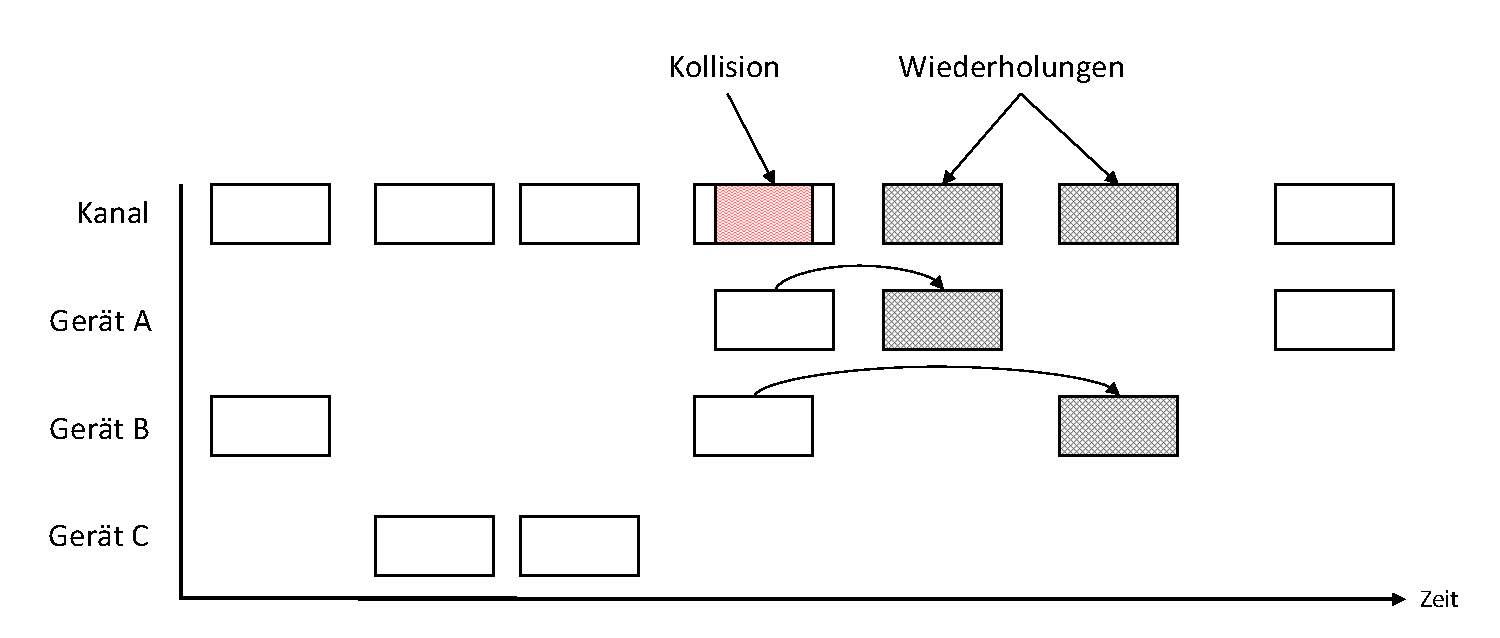
\includegraphics[width=1\linewidth]{gfx/ALOHA}} 
        \caption[ALOHA]{Beispiel für den Kanlazugriff nach dem ALOHA Protokoll }\label{fig:aloha}
\end{figure}

Die wiederholten Sendevorgänge wirken sich ungünstig auf den Energieverbrauch der \glspl{node} aus. Mit steigender Anzahl der Teilnehmer, wie es in Logistanwendungen der Fall ist, stößt dieses System an seine Grenzen \citep{inBinTestbed}. 

\section{Listen Before Talk}\label{kap:zugriffsverfahren_sec:lbt}
Das \emph{\ac{etsi}} befasst sich in \citep{lbt} mit der elektromagnetischen Verträglichkeit und der Nutzung des Funkspektrums durch \acp{srd}. Um die Ausnutzung des Funkkanals als begrenzte physikalische Ressource zu maximieren, beschreibt dieser Standard einen \ac{lbt} Kanalzugriff. 

Ist ein Gerät im Begriff, eine Übertragung zu starten, soll es zunächst den Funkkanal nach Aktivitäten anderer Geräte abhören und die eigentliche Übertragung noch zurückhalten. Die Abhörzeit $t_{\textrm{L}}$ setzt sich aus einer festen und einer zufälligen Komponente zusammen:
\begin{equation}
{t_{\textrm{L}}} = {t_{\textrm{F}}} + {t_{\textrm{PS}}}
\end{equation}
${t_{\textrm{F}}}$ beträgt $5ms$, während ${t_{\textrm{PS}}}$ einen zufälligen Wert zwischen $0ms$ und $5ms$ annimmt. Wird innerhalb von ${t_{\textrm{F}}}$ keine Aktivität erkannt, beginnt der Sendevorgang direkt im Anschluss und ${t_{\textrm{PS}}}$ wird zu $0$ gesetzt. Wohingegen im Fall eines belegten Kanals die Abhörzeit unterbrochen wird bis der Kanal wieder frei ist. Im Anschluss wird der Kanal für die gesamte Dauer von ${t_{\textrm{L}}}$ abgehört, die durch den Anteil von ${t_{\textrm{PS}}}$ variieren kann. \autoref{fig:lbt} verdeutlicht diese Verfahren exemplarisch für drei Geräte. \texttt{Gerät C} detektiert keine Aktivität auf dem Kanal innerhalb der $5ms$ Abhörzeit und startet daher unverzüglich mit der Übertragung. \texttt{Gerät B} und \texttt{Gerät A}, die zu diesem Zeitpunkt jeweils eine Übertragung ausstehen haben, können diese erst nach zwei bzw. drei Abhörzyklen beginnen.

In \autoref{fig:lbt} wird auch deutlich, wann sich die Geräte im Sende- , bzw. Empfangsmodus befinden. Um den Kanal abzuhören, muss sich ein Gerät im Empfangsmodus befinden. Der \ac{lbt} Algorithmus sieht vor, dass im Fall eines belegten Kanals solange gewartet wird, bis dieser wieder frei ist. Auch in dieser Zeit muss ein Gerät im Empfangsstatus verbleiben, um den Zeitpunkt festzustellen, wann der Kanal wieder frei ist und der Backoff-Mechanismus erneut gestartet werden kann. Im Vergleich zu \texttt{Gerät C} ergibt sich für \texttt{Gerät A} eine erheblich längere Zeitspanne im Empfangsmodus.

\begin{figure}[bth]
        \myfloatalign
        {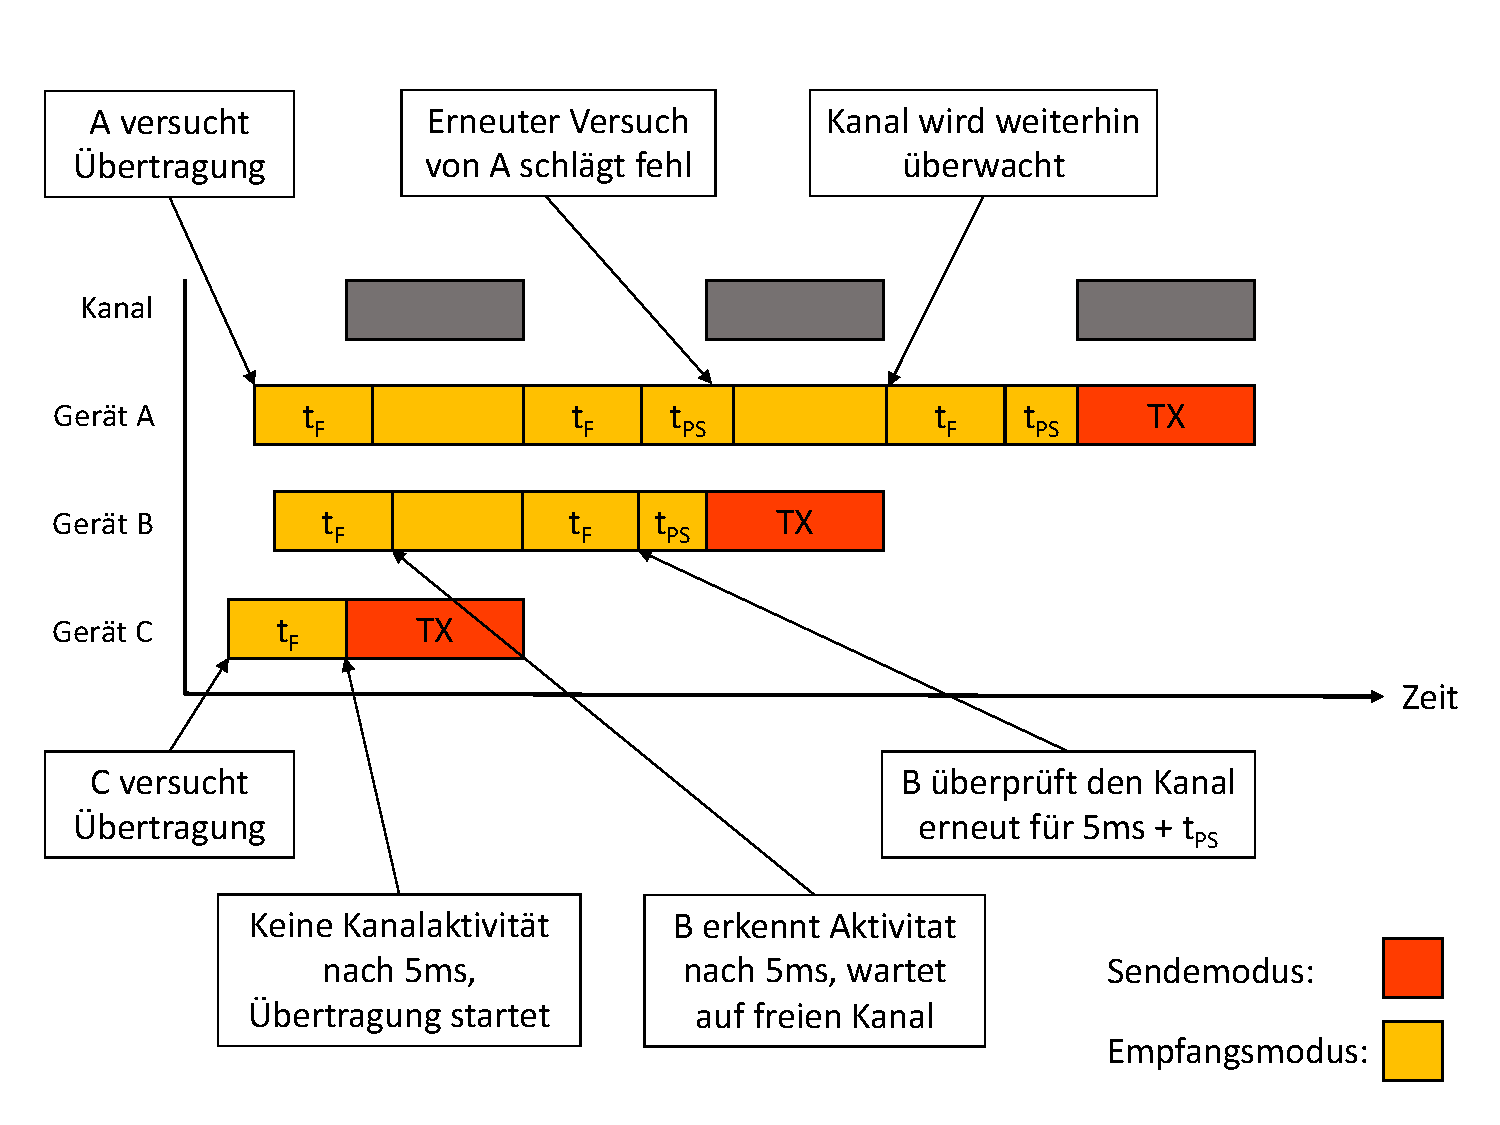
\includegraphics[width=1\linewidth]{gfx/LBT}} 
        \caption[Listen Before Talk]{Beispiel für den LBT Algorithmus bei drei konkurrierenden Kanalzugriffen. Die orange markierten Zeiten repräsentieren Empfangsstatus, die roten Sendestatus.}\label{fig:lbt}
\end{figure}

\section{Carrier Sense Multiple Access / Collision Avoidance}\label{kap:zugriffsverfahren_sec:csma}
Das \ac{ieee} standardisiert in \cite{ieee} die Bitübertragung (\emph{Physical Layer}) und den Kanalzugriff (\acs{mac}-\emph{Layer}) als Teil der Verbindungssicherung\footnote{im Bezug auf das \acl{osi} Referenzmodell der \acs{iso}} für Sensornetzwerke mit niedriger Datenrate. Das Protokoll sieht vor, dass vor Beginn einer Übertragung ein \acl{csma} Algorithmus durchlaufen wird. Ähnlich dem \acs{lbt} sieht dieser vor, eine Übertragung zunächst nach einem bestimmten Muster zurückzuhalten. Dieser Vorgang wird \emph{Backoff} genannt. In der Grundversion muss ein Gerät zwei Variablen zur Durchführung des Algorithmus verwalten:
\begin{enumerate}
	\item $NB$: Anzahl der Durchläufe des Algorithmus für den aktuellen Sendeversuch
	\item $BE$: Backoff-Exponent, der den Backoff-Zeitraum eingrenzt
\end{enumerate}
Alle Zeitangaben, die in dem Standard beschrieben werden, beziehen sich auf die Übertragungsdauer eines Symbols, die \emph{Symbol Period}. Dem \acs{csma} Verfahren liegt der Einheitszeitraum \emph{Unit Backoff Period} zugrunde, der aus 20 \emph{Symbol Periods} besteht \cite{ieee}. Mit den in dieser Arbeit gewählten Einstellungen\footnote{Symbolrate = $20 \frac{kSymbols}{s}$, (Bitrate = $20 \frac{kBit}{s}$, BPSK Modulation)} ergibt sich:
\begin{center}
\emph{Unit Backoff Period} $ = 1ms$
\end{center}
Die Backoff-Zeiten sind ganzzahlige Vielfache dieses Zeitraums und  werden zufällig bestimmt. Die Menge der möglichen Werte ist: 
\begin{center}
$\{0, (2\textsuperscript{BE})-1)\}$  \emph{Unit Backoff Periods}
\end{center}
Die Variable $BE$ begrenzt somit die Auswahl der möglichen Backoff-Zeiten. Ein Blockdiagramm des Algorithmus ist in \autoref{ahg:csmablock} zu sehen. In \autoref{fig:csma} ist das Verfahren exemplarisch mit drei konkurrierenden Sendeversuchen dargestellt. Jedes Gerät hält seine Übertragung zunächst für eine zufällige Zeit, wie zuvor beschrieben, zurück. Im Anschluss wird die Aktivität auf dem Funkkanal überprüft (\acf{cca}). Die Prüfung des Kanals soll nach \citep{ieee} $0,4ms$ dauern. In \autoref{fig:csma} stellt Gerät B nach der Kanalprüfung keine Aktivität fest und beginnt mit dem Sendevorgang. Für dieses Gerät hat der Algorithmus an dieser Stelle erfolgreich terminiert. Die Kanalprüfung der Geräte A und C fällt negativ aus, sodass der Algorithmus die nächste Iteration durchläuft. Dabei werden nun die Variablen $NB$ und $BE$ jeweils um eins erhöht, wie \autoref{ahg:csmablock} zu entnehmen ist. Dadurch steigt die Anzahl der möglichen Backoff-Zeiten mit jedem Durchlauf. Dies bedeutet nicht, dass die konkreten Backoff-Zeiten stetig größer werden, es stehen nur mehrere verschiedene Zeiträume zur Verfügung.
Anzumerken ist, dass sich die Geräte während des Backoffs nicht im Empfangsstatus befinden müssen. 

\begin{figure}[bth]
        \myfloatalign
        {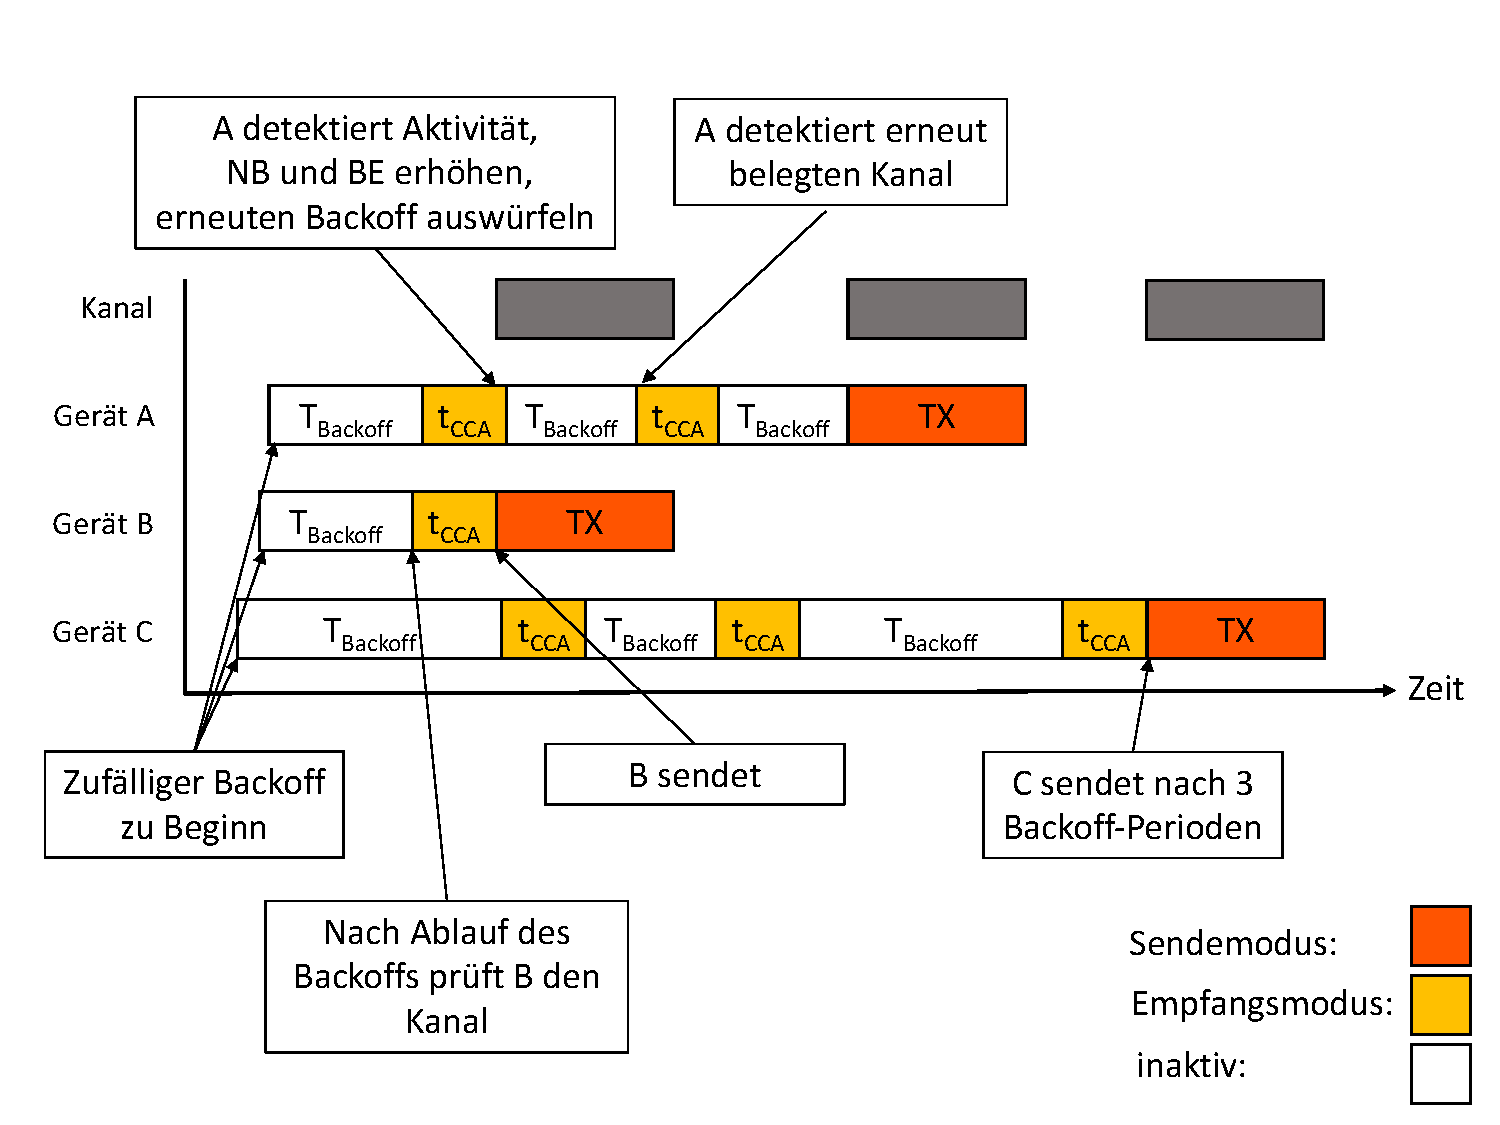
\includegraphics[width=1\linewidth]{gfx/CSMA}} 
        \caption[Carrier Sense Multiple Access]{Beispiel für den CSMA-CA Algorithmus bei drei konkurrierenden Kanalzuriffen. Die orange markierten Zeiten repräsentieren Empfangsmodus, die roten Sendemodus. Während der weiß markierten Zeiten ist kein aktiver Modus notwendig. }\label{fig:csma}
\end{figure}

\section{Schlussfolgerung für die weitere Untersuchung}

Ein unkoordinierter Kanalzugriff nach dem ALOHA Ansatz führt bei einer großen Teilnehmeranzahl zu vielen Kollisionen. Übertragungen müssen dann wiederholt werden, was sich negativ auf den Energieverbrauch auswirkt. Dieser Ansatz ist daher für den Einsatz in einem großskaligen \acs{wsn} mit stark eingeschränkter Energieverfügbarkeit der \glspl{node} nicht geeignet \cite{inBinTestbed}. 

Die eine genaue Untersuchung des \acs{lbt} und des \acs{csma} Verfahrens sind dagegen in Erwägung zu ziehen \cite{Falkenberg2017b}\citep{GreenOrbs}. Im Vergleich von \autoref{fig:lbt} und \autoref{fig:csma} wird jedoch deutlich, dass der \acs{csma} Algorithmus hinsichtlich der Energieeffizienz deutliche Vorteile aufweist. Der dramatische Anstieg des mittleren Energieverbrauchs pro \gls{node} bei Verwendung von \acs{lbt} wird in \citep{Falkenberg2017b} demonstriert.
Daher wird im Folgenden das \acs{csma} Zugriffsverfahren nach dem \gls{802154} Standard näher untersucht. 

%*****************************************
%*****************************************
%*****************************************
%*****************************************
%*****************************************





%************************************************
\chapter{Systembeschreibung und Analysemethode}\label{kap:systembeschreibung}
%************************************************

Dieses Kapitel gliedert sich in zwei Teile. Im ersten Teil werden zum Zweck der Vergleichbarkeit die Rahmenbedingungen der in \autoref{kap:simulation} beschriebenen Simulation festgelegt, der zweite Teil beschäftigt sich mit der Analysemethode und definiert Messgrößen für die spätere Bewertung der Ergebnisse.

\section{Ein geeignetes Szenario}
\begin{figure}[bth]
        \myfloatalign
        {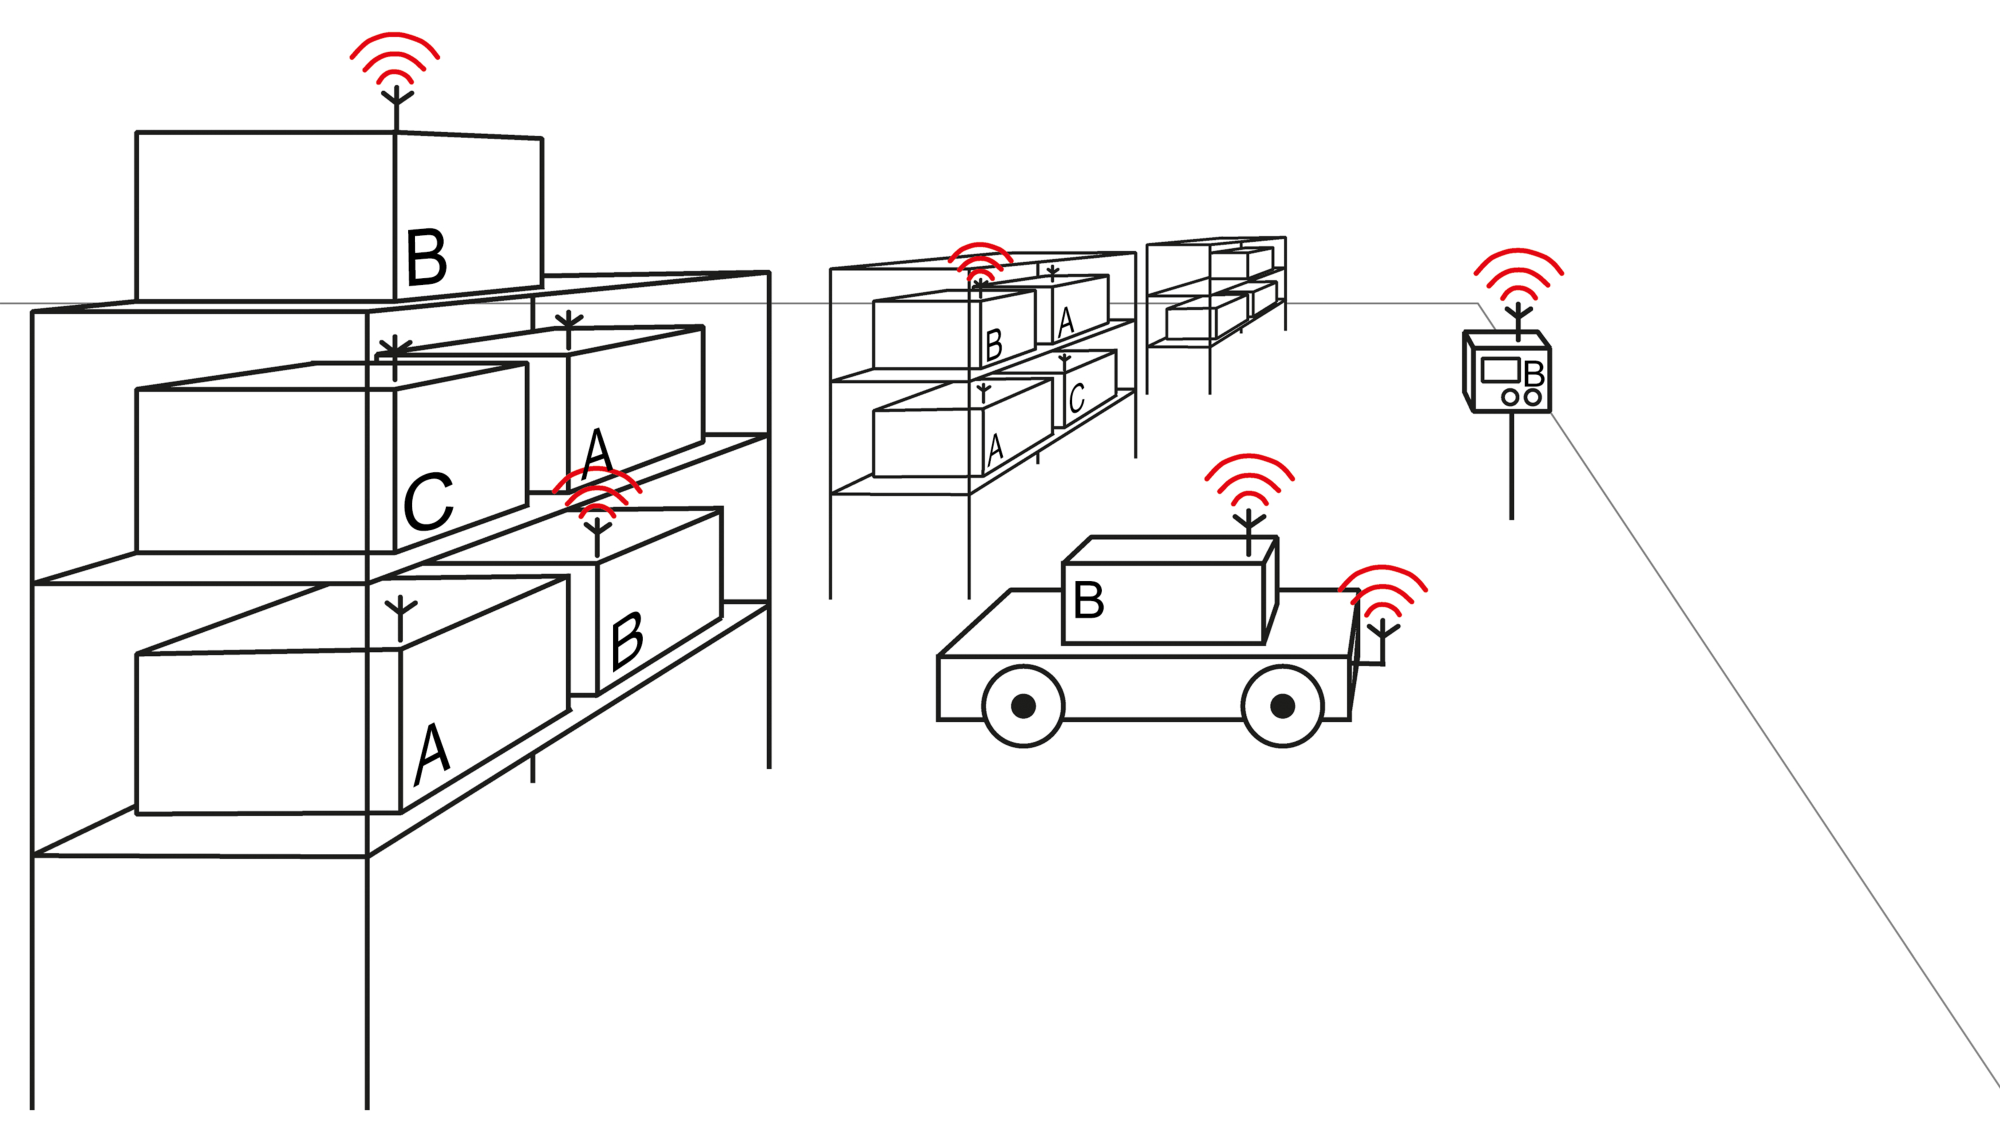
\includegraphics[width=1\linewidth]{gfx/uebersicht}} 
        \caption[Scenario]{Beispiel für ein Logistikszenario mit vernetzten Frachtcontainern. Die Beschriftungen A, B, C stehen für drei verschiedene Produkte}\label{fig:lageruebersicht}
\end{figure}
Hauptbestandteil eines intelligenten Logistiklagers sind die Frachtcontainer mit den verschiedenen Gütern. Daneben gibt es Systeme zur Beförderung und Einlagerung der Frachtcontainer, dafür können auch mobile Roboter zu Einsatz kommen, wie in \autoref{fig:lageruebersicht} angedeutet. Dienstprogramme, wie eine automatische Inventarisierung oder Kommissionierung, also das Zusammenstellen von bestimmten Produkten für einen Auftrag, gehören ebenfalls zu  einem selbst organisierten Warenlager. Sowohl die Systeme zur Beförderung als auch die Computer, auf denen die Dienstprogramme ausgeführt werden, müssen in der Lage sein, mit den Frachtcontainern zu kommunizieren. Sie werden damit Teil des Funknetzwerkes. Üblicherweise sind in einen Kommunikationsprozess die Container involviert, die das gleiche Produkt oder eine bestimmte Kategorie an Frachtgütern beinhalten. In \autoref{fig:lageruebersicht} hat \zB gerade ein Kommunikationsprozess bezogen auf das Produkt B begonnen. Charakteristisch ist, dass dabei eine Anfrage von einer Stelle ausgeht und für eine Vielzahl an Empfängern --- den Frachtcontainern --- bestimmt ist, die diese Anfrage beantworten. Von welcher Quelle genau die Anfrage stammt, ist für die Funktion des Kanalzugriffverfahren unerheblich, da sich immer o.g. Muster ergibt. Eine mobile Transporteinheit, die den kürzesten Weg zu einem Produkt finden möchte, oder eine Verfügbarkeitsanfrage über das Internet sind nur zwei Beispiele.

\subsection{Anordnung}
Als Grundlage für die spätere Simulation wird ein Anordnung angenommen, die der typischen Platzierung von Frachtcontainern in Logistiklagern entspricht. Dabei werden die Container in mehreren Zeilen von Hochregalen eingelagert, sodass sich die \glspl{node} des zu untersuchenden \ac{wsn} in einer dreidimensionalen Matrix befinden. 

\begin{figure}[bth]
        \myfloatalign
        {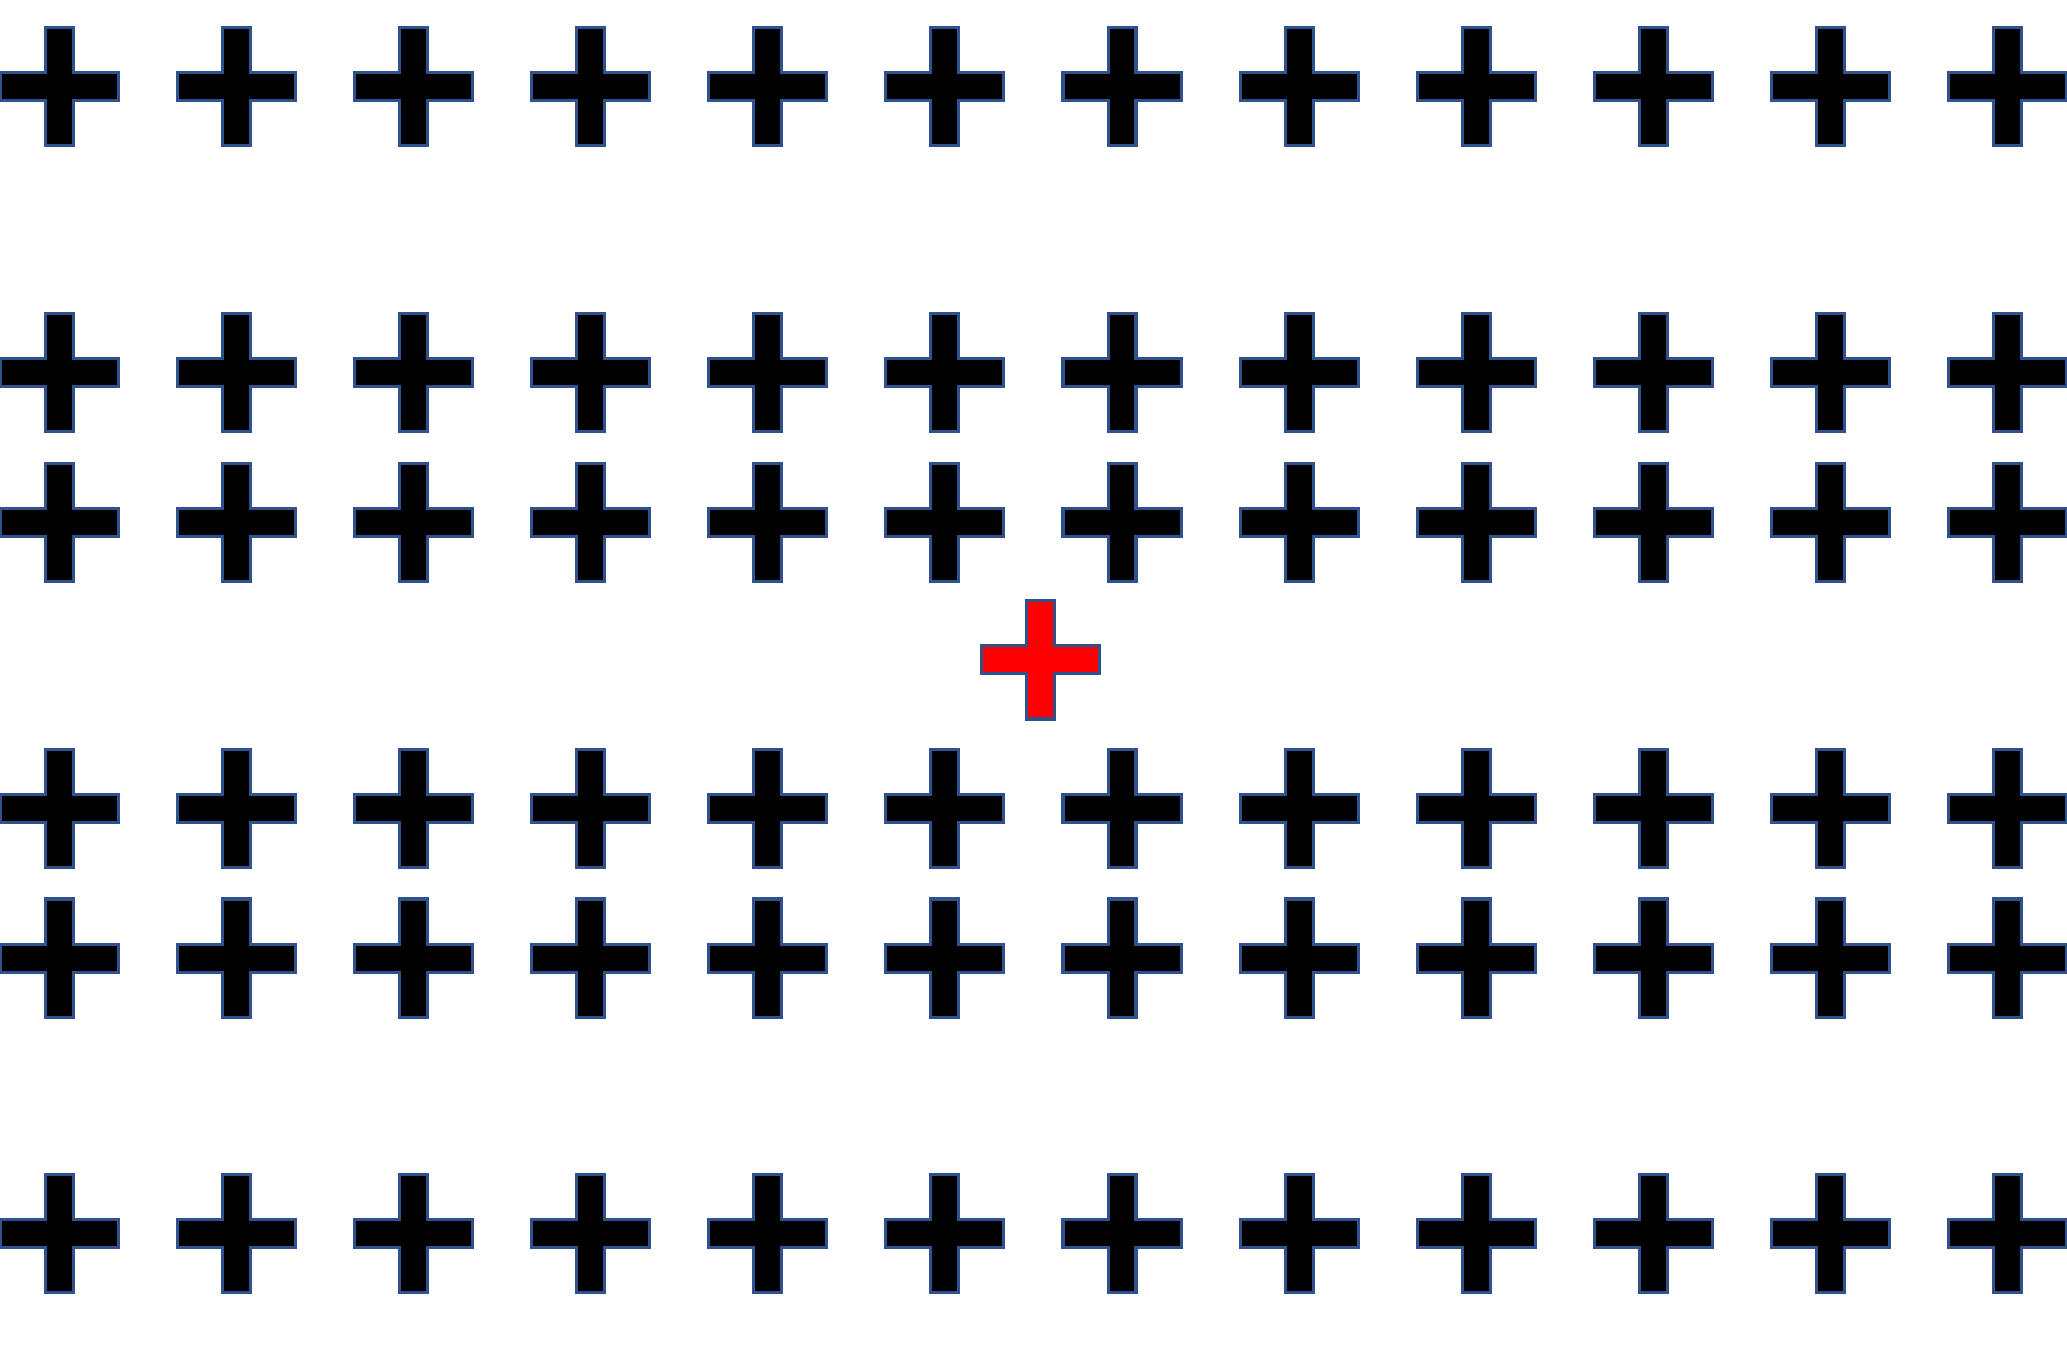
\includegraphics[width=0.5\linewidth]{gfx/anordnung}} 
        \caption[Anordnung von Frachtcontainern in einem Logistiklager]{Die einzelnen Frachtcontainer werden in einem Logistiklager in Hochregalen zeilenweise eingelagert. Die Grafik zeigt die Aufsicht der Containerpositionen. An der rot markierten Position befindet sich der \acs{ap}}\label{fig:lager}
\end{figure}

Weiterhin wird in dieser Arbeit angenommen, dass es einen einzelnen Funkknoten gibt dessen Reichweite das gesamte Lager abdeckt und im weiteren Verlauf dieser Arbeit als \ac{ap} bezeichnet wird. Eine Anordnung mit mehreren \acp{ap} zur Reduzierung der Sendeleistungen ist sinnvoll \citep{Falkenberg2017b}, jedoch hier nicht Gegenstand der Untersuchung. Die Beobachtungen hinsichtlich der Netzlast in dem hier gewählten Ansatz lassen sich unter Berücksichtigung von Überlappungen auf ein Szenario mit mehreren \acsp{ap} übertragen. \autoref{fig:lager} zeigt diese Anordnung aus der Aufsicht.

\subsection{Energieversorgung}
Für die spätere Bewertung der Energiebilanz wird angenommen, dass der \ac{ap} über eine unkritische Energieversorgung verfügt --- \zB direkt an das Stromnetz angeschlossen ist. Dagegen steht an den einzelnen \glspl{node} nur eine sehr begrenzte Menge an Energie zu Verfügung, mit der effizient zu haushalten ist \cite{inBin}.

\subsection{Datenaufkommen} \label{kap:systembeschreibung_sek:datenaufkommen}
Um die Paketgröße der ausgetauschten Nachrichten abzuschätzen, werden die folgenden Punkte berücksichtigt:
\begin{description}
	\item[Identifizierung des Frachtcontainers] Um einen Frachtcontainer zu identifizieren, ist eine eindeutige Adresse notwendig. Hier bietet sich die \ac{mac} Adresse an, die im  IEEE 802.15.4 Standard verwendet wird \cite{ieee}. Diese ist acht Byte lang \cite[151]{ieee}.
	\item[Identifikation des Frachtgutes] Wie in \citep{inBin} beschrieben, werden Güter in automatisierten Logistikprozessen mit der \acs{rfid}-Technologie identifiziert. Hierbei wird der \acf{epc} des Produkts ausgelesen. Zur Identifizierung eines einzelnen Produkts dient die \acf{gtin}, die typischerweise in einem Strichcode codiert ist. Da die  \acs{rfid}-Technologie aber auch das berührungslose Auslesen von größeren Gebinden erlaubt, enthält der \acs{epc} zusätzlich Informationen über die logistische Einheit, wie \zB Verpackungseinheit oder Palette. Der \acs{epc} besteht in der gebräuchlichsten Form aus 12 Byte \citep{epc}. 
	\item[Nachrichten Typ] Die unterschiedlichen Nachrichten-Arten können in einem Byte codiert werden. Das erlaubt theoretisch bis zu 256 verschiedene Nachrichtenarten oder das Verwenden von einzelnen Bits innerhalb dieses Bytes für Steuerinformationen, \zB Sequenznummern.
	\item[Parameter] Dieser Teil der Nachricht bietet Platz für zusätzliche Informationen je nach Nachrichtenart und wird pauschal mit zwei Byte veranschlagt.
\end{description}

Die genannten Punkte bilden die wesentlichen Bestandteile für den Informationsaustausch innerhalb eines Logistklagers. \autoref{tab:pktlen} gibt einen Überblick über die resultierende Paketlänge. Es wird hierbei davon ausgegangen, dass eine Nachricht in der Regel alle Felder, jedoch mindestens Nachrichten-Typ und ein weiteres Feld enthält. Daher wird in \autoref{fig:frame} ein Nachrichtenrahmen mit fester Länge definiert.

\begin{table}
    \myfloatalign
  \begin{tabularx}{0.7\textwidth}{Xll} \toprule
    \tableheadline{Feld} & \tableheadline{Länge in Byte} \\ \midrule
    Node ID $($\acs{mac}-Adresse$)$ & 8 \\
    Produkt ID $($\acs{epc}$)$ & 12 \\
    Nachrichten-Typ & 1 \\
    Parameter & 2 \\
    \midrule
    Summe & 23 \\
    \bottomrule
  \end{tabularx}
  \caption[Nachrichtenfelder]{Bestandteile einer exemplarischen Nachricht für die Kommunikation in Logistiklagern}  \label{tab:pktlen}
\end{table}

\begin{figure}[bth]
        \myfloatalign
        {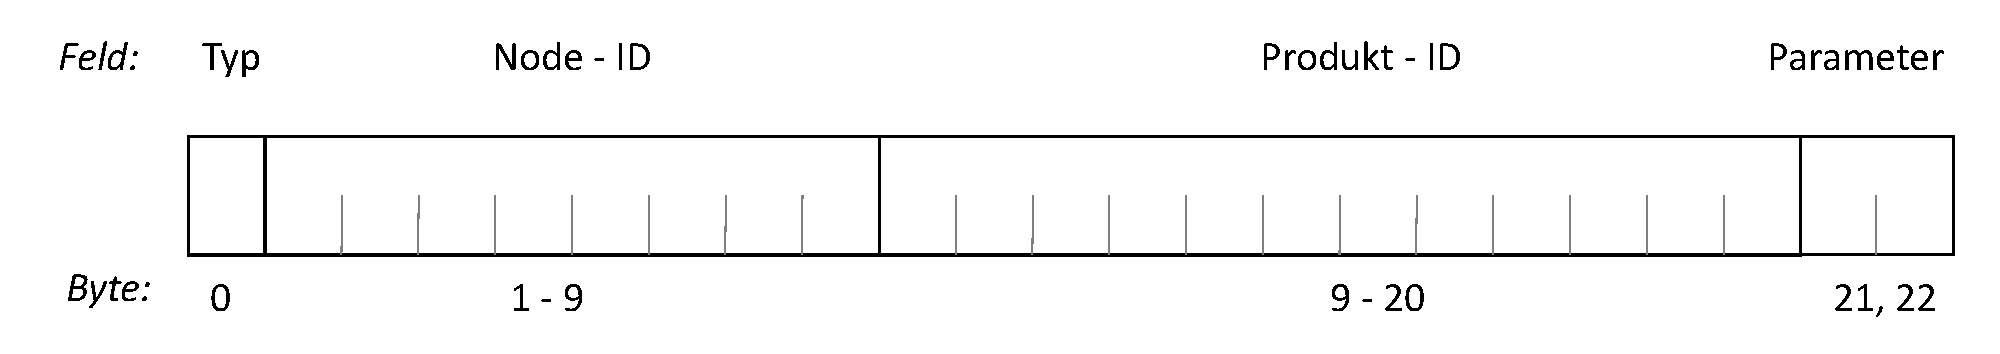
\includegraphics[width=1\linewidth]{gfx/Frame-Muster}} 
        \caption[Nachrichtenrahmen]{Nachrichtenrahmen mit fester Länge für den Informationsaustausch im Logistiklager}\label{fig:frame}
\end{figure}


\subsection{Kommunikationsfluss}
Die zwei Kernpunkte des Informationsaustausches für das zu untersuchende Szenario sind:
\begin{enumerate}
\item Anfragen nach einem bestimmten Produkt
\item Meldung der Frachtcontainer über deren Inhalt
\end{enumerate}
Darüber hinaus sind weitere Nachrichten zur Organisation nötig, wie etwa:
\begin{aenumerate}
\item Anmeldung neuer Frachtcontainer
\item Zuweisung eines Produktes zu einem Frachtcontainer
\item Meldung der Frachtcontainer über geringen Warenbestand
\item Fehlermeldungen
\end{aenumerate}
Für die Untersuchung eines leistungsfähigen Kanalzugriffprotokolls spielen diese Nachrichten jedoch eine untergeordnete Rolle. Die Erprobung des Kanlzugriffprotokolls bezieht sich auf einen \emph{Anfrage-Antwort} Zyklus, der vom \acs{ap} initiiert wird. Dazu werden in \autoref{fig:nachrichten} zwei Nachrichtentypen nach dem Schema aus \autoref{kap:systembeschreibung_sek:datenaufkommen} definiert. Der erste Typ ist \emph{PAGE} und dient der Anfrage nach einem Produkt, der zweite Typ heißt \emph{QUANTITY} und ist für die Antworten der Frachtcontainer vorgesehen. Die PAGE-Nachricht wird als Broadcast in das Netz geschickt und löst damit nahezu gleichzeitige QUANTITY-Nachrichten der \glspl{node} aus. Im Gegensatz zu \cite{inBinTestbed} wird von regelmäßigen Status-Nachrichten von Seiten der Frachtcontainer abgesehen. Der Ablauf eines Kommunikationszyklus ist in \autoref{fig:sequenz} als Sequenzdiagramm dargestellt.

\begin{figure}[bth]
        \myfloatalign
        \subfloat[Typ 1 Nachricht: PAGE]
        {\label{fig:nachrichten-a}%
         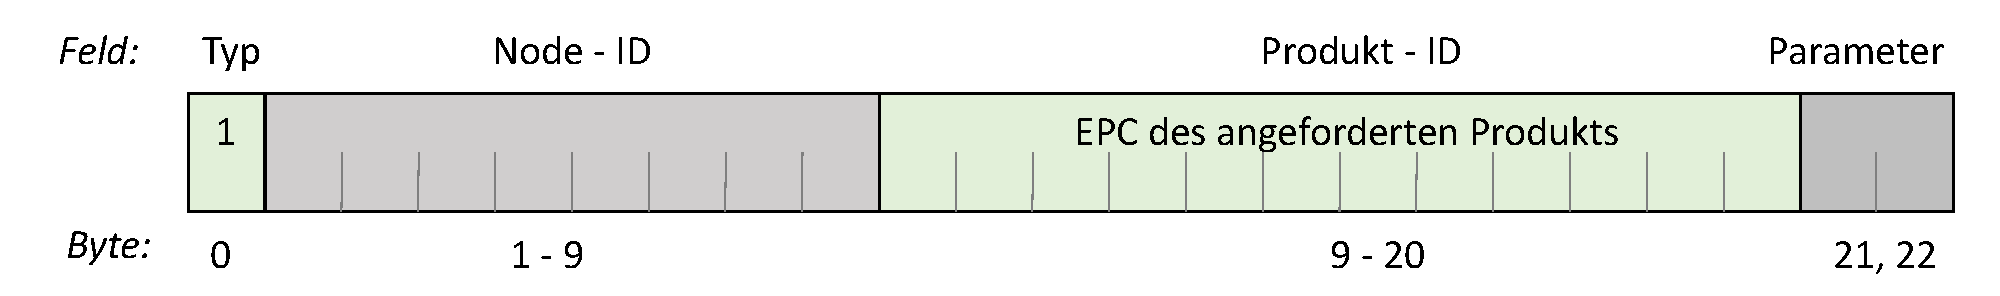
\includegraphics[width=1\linewidth]{gfx/Page-Frame}} \\
        \subfloat[Typ 2 Nachricht: QUANTITY]
        {\label{fig:nachrichten-b}%
        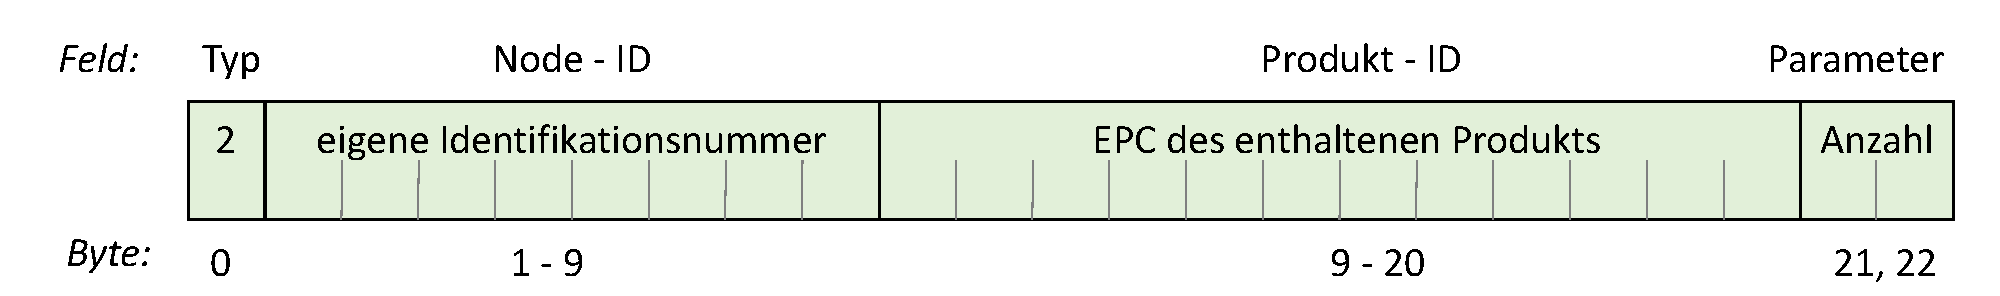
\includegraphics[width=1\linewidth]{gfx/Quantity-Frame}} 
        \caption[Nachrichtentypen]{Nachrichtentypen zur Abfrage von bestimmen Produkten. a) PAGE Nachricht mit angefordertem Produkt. b) QUANTITY Nachricht mit Anzahl der im Frachtcontainer verfügbaren Menge.}\label{fig:nachrichten}
\end{figure}

\begin{figure}[bth]
        \myfloatalign
        {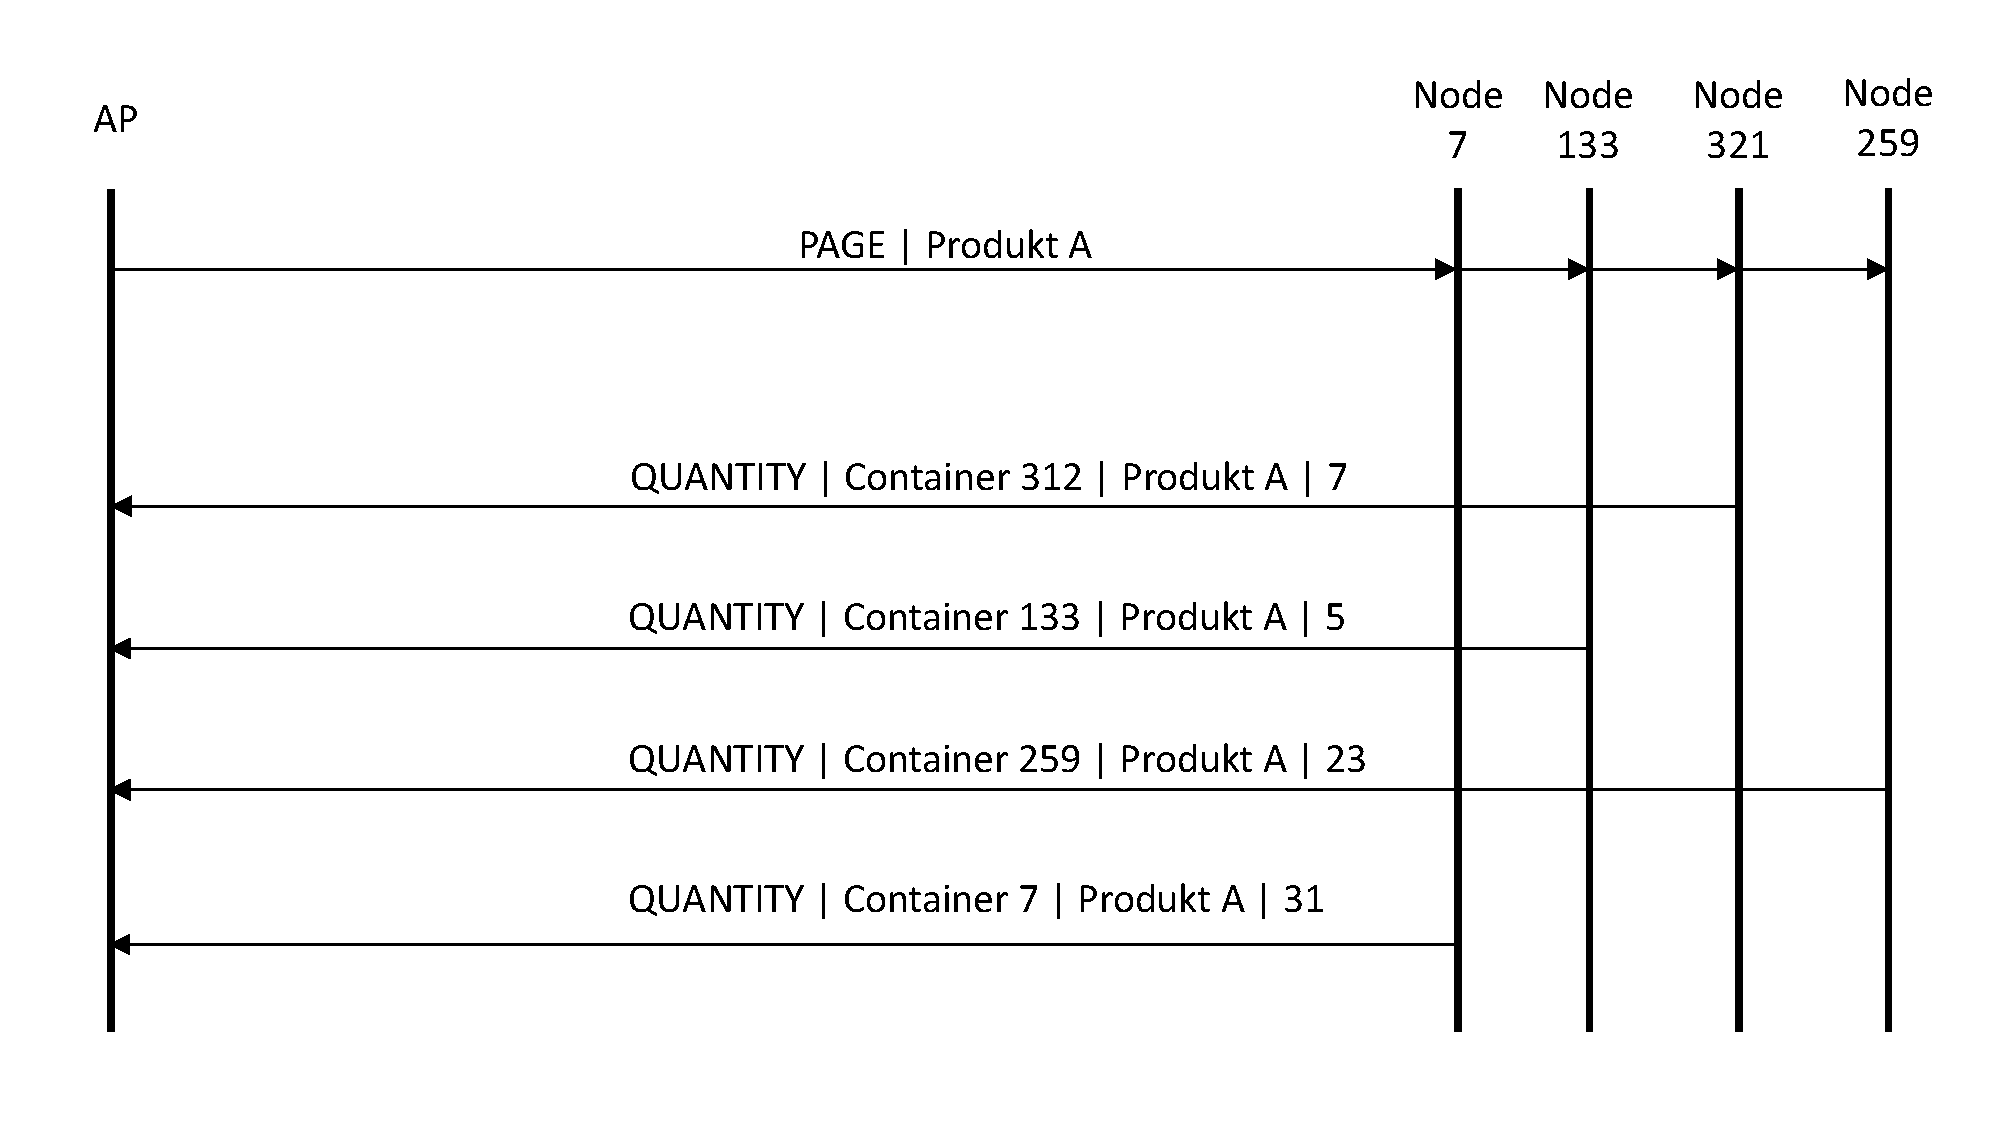
\includegraphics[width=1\linewidth]{gfx/Sequenzdiagramm}} 
        \caption[Sequenzdiagramm]{Sequenzdiagramm der Nachrichten zwischen \acs{ap} und \glspl{node} bei einer Produktanfrage}\label{fig:sequenz}
\end{figure}

Wie in \autoref{kap:verwandtearbeiten} aufgezeigt, sinkt die Leitungsfähigkeit der Systeme in \citep{GreenOrbs} und \citep{inBinTestbed} mit steigender Anzahl an parallelen Vorgängen innerhalb des Netzwerkes. Die Wahl des oben beschriebenen Kommunikationsflusses provoziert diese parallelen Vorgänge durch die hohe Zahl nahezu gleichzeitig versandter \emph{QUANTITY}-Nachrichten und ist daher zur Untersuchung der Kanalzugriffverfahrens geeignet.

Anzumerken ist, dass eine Anfrage über den \ac{ap} immer ein bestimmtes Produkt betrifft. Somit antwortet nur eine Teilmenge der sich insgesamt im Lager befindlichen Frachtcontainer.
Die Ergebnisse dieser Arbeit können daher auch zu einer optimalen Verteilung einer Ware auf Frachtcontainer genutzt werden.


\subsection{Kanalmodell}
Im hier untersuchten Szenario wird als Kanalmodell die Freiraumausbreitung angenommen. 
Eine Analyse mit anderen Kanalmodellen ist zwar nicht Gegenstand dieser Arbeit, die Simulation erlaubt jedoch den Austausch des Kanalmodells für künftige Untersuchungen.

\section{Analyse- und Messmethode}

Ein zentrales Kriterium zur Beurteilung der Leistungsfähigkeit eines Kanalzugriffverfahrens in dem geschilderten Szenario ist die Anzahl an \emph{QUANTITY}-Nachrichten, die nach einer \emph{PAGE}-Nachricht beim \acs{ap} ankommen. Weiterhin ist für die Bewertung der Energieeffizienz des Protokolls der Energieverbrauch an den einzelnen \glspl{node} relevant.
Weiterhin ist die Zeitspanne relevant, nach welcher der \acs{ap} alle Nachrichten empfangen hat. Im Folgenden werden dazu Messgrößen für die Simulation definiert.

\paragraph{Product Specific Delivery Ratio} Die \acf{psdr} bezieht die am \acs{ap} erfolgreich empfangenen Antworten auf die Anzahl der Frachtcontainer mit gleichem Produkt:
\begin{equation}
{r_\textrm{PS}} = \frac{N_\textrm{Antworten}}{N_\textrm{Container mit gleichem Produkt}}
\end{equation}

\paragraph{Mittlerer Energieverbrauch}
.. TODO ..
Bespr. mit Robert, 
passive knoten ausgelassen, da Energieverbrauch unabhängig von Kanalzugriff .. sniffen sowieso nur minimalistisch auf dem kanal

Kanalauslastung

\subsection{Messaufbau}\label{kap:systembeschreibung_sec:analyseaufbau}

\begin{figure}[bth]
        \myfloatalign
        {\includegraphics[width=1\linewidth]{gfx/Analyseaufbau}} 
        \caption[Ananlyseaufbau]{ToDo}\label{fig:sequenz}
\end{figure}

\begin{aenumerate}
\item \emph{PowerScale} System zur Messung des Energieverbrauchs am \gls{node}
\item \emph{Code Composer Studio} Entwicklungsumgebung zur Ausführungssteuerung Prototypenprogramms
\item \emph{Packet Sniffer} Analysesoftware zum Auslesen des CC1200 Funkchips
\item \emph{Real Time Spectrum Analyzer} Messgerät zur kontinuierlichen Anzeige der momentanen Signalstärke im eingestellten Frequenzbereich
\item \emph{hterm} Terminalpraogramm zum seriellen Datenaustausch mit dem \acs{ap}

\end{aenumerate}



%*****************************************
%*****************************************
%*****************************************
%*****************************************
%*****************************************





%************************************************
\chapter{Simulation}\label{kap:simulation}
%************************************************
\section{IEEE 802.15.4 Modell}\label{kap:simulation_sec:beschreibung}
Beschreibung, Aufbau \\
Besonders wichtig : Modellierung des Funkkanals \\
Beschreibung des Fehlers in der Datensammlung für Kollisionen \\
Bewertung des Modells für die Verwendung in dieser Arbeit \\

\section{Erweiterungen des Modells}\label{kap:simulation_sec:erweiterung}
Austausch/Neuerstellung der Anwendungsschicht \\
Ergänzung um automatische, zufällige Platzierung der Container \\
Besonders wichtig: Anpassung der Transceivermodi -> Energiemodell \\
--> Einbindung realer Messwerte \\

\section{Simulationsergebnisse}\label{kap:simulation_sec:ergebnisse}
\begin{figure}[bth]
        \myfloatalign
        {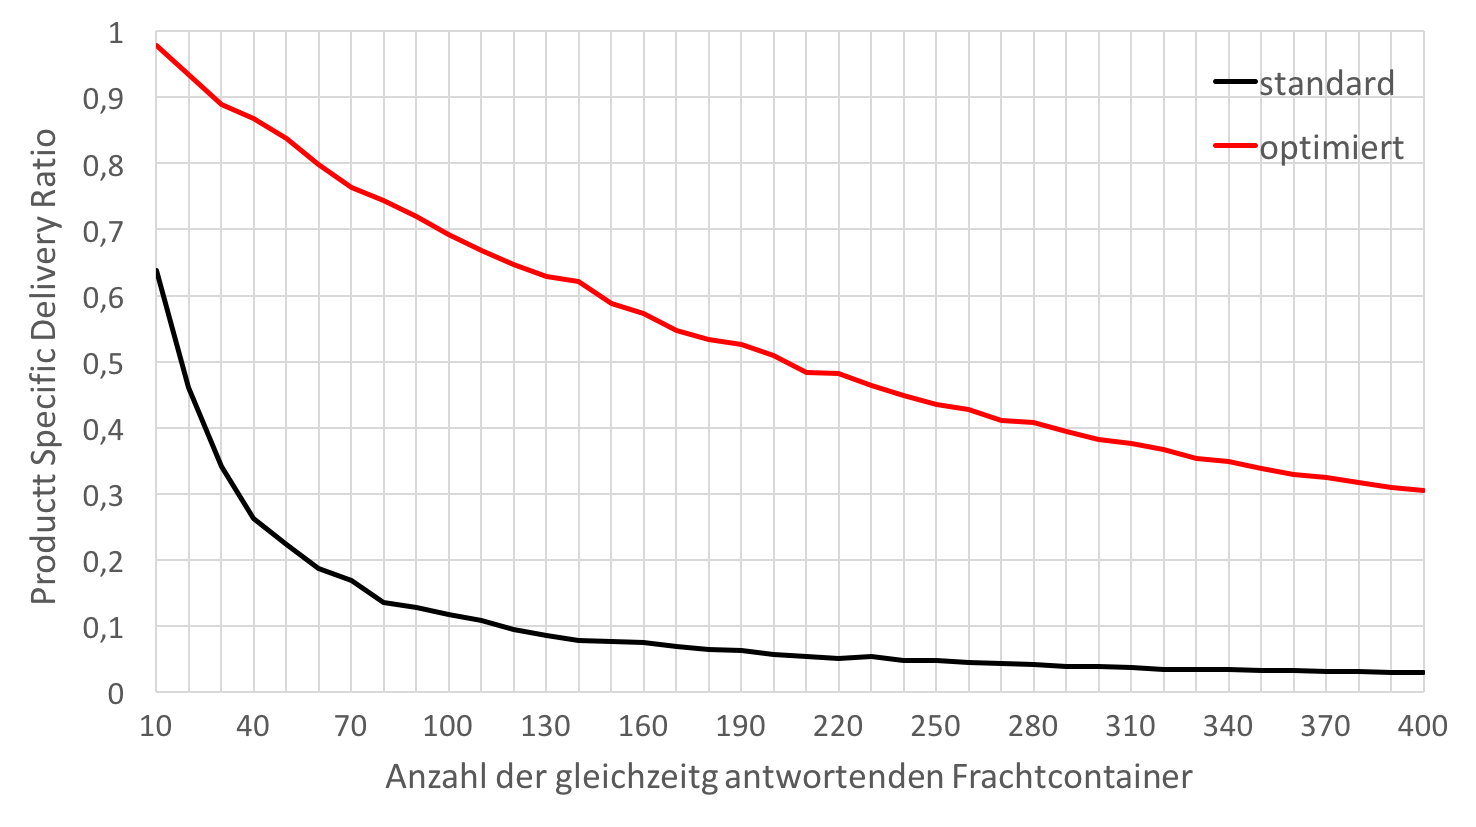
\includegraphics[width=1\linewidth]{gfx/Diag_Durchsatz_10_400}} 
        \caption[Durchsatz]{ToDo}\label{fig:diag_durchsatz_10_400}
\end{figure}

Beschreibung -> näherungsweise neg.exp. \\
Konvergenz interessant evtl. noch ein Durchlauf bis 1000 \\
Begründung des höheren Durchsatzes: Erleuterung der Auswahl von BE \\
evtl. Statistik mit einbeziehen \\

\begin{figure}[bth]
        \myfloatalign
        {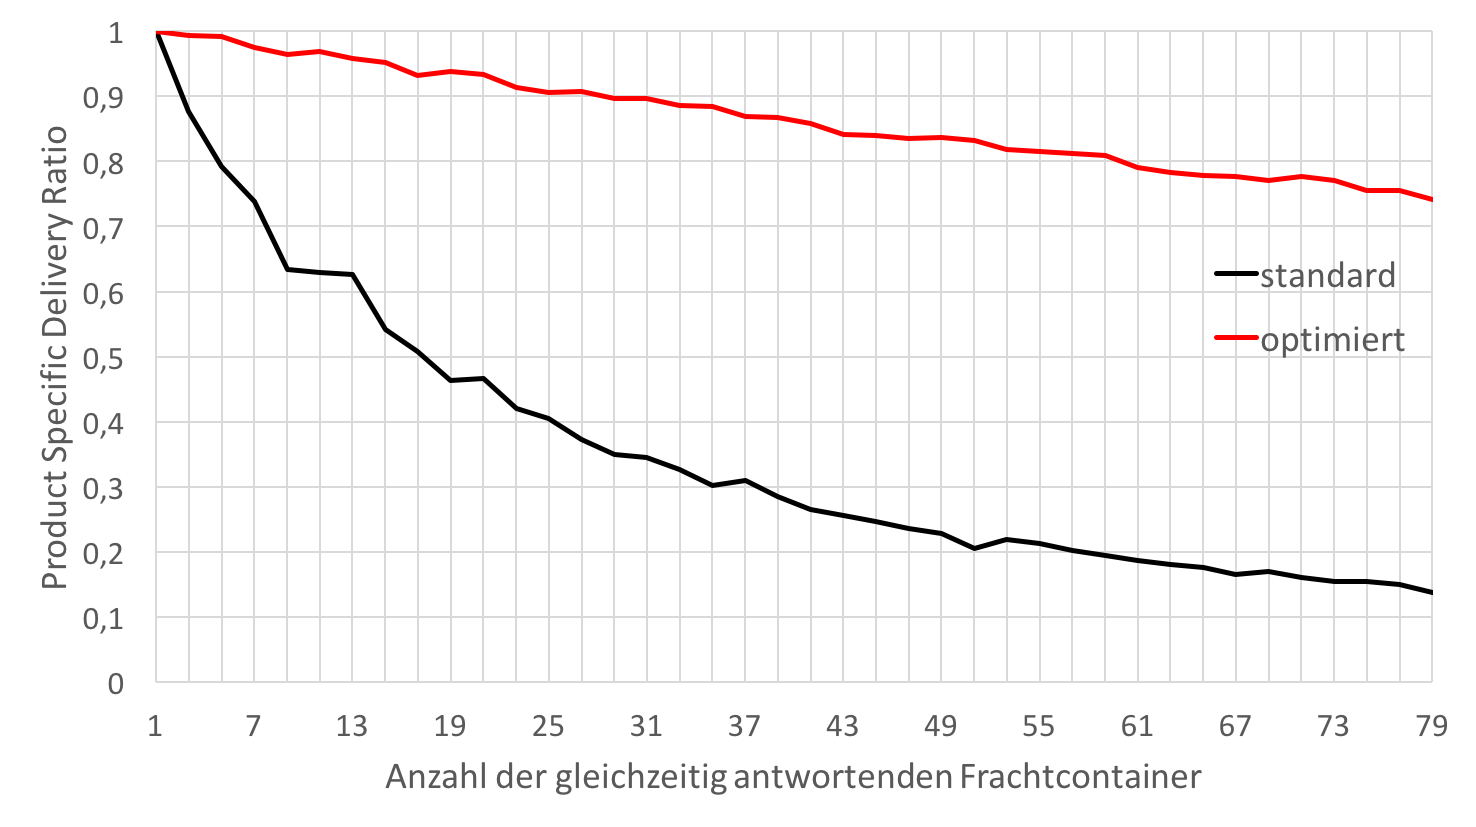
\includegraphics[width=1\linewidth]{gfx/Diag_Durchsatz_1_80}} 
        \caption[Durchsatz im Detail]{ToDo}\label{fig:diag_durchsatz_1_80}
\end{figure}

besonders effizient im Bereich bis ca. 80 Sendern \\
bei standard bereist bei wenigen Sendern massive Kollisionen

\begin{figure}[bth]
        \myfloatalign
        {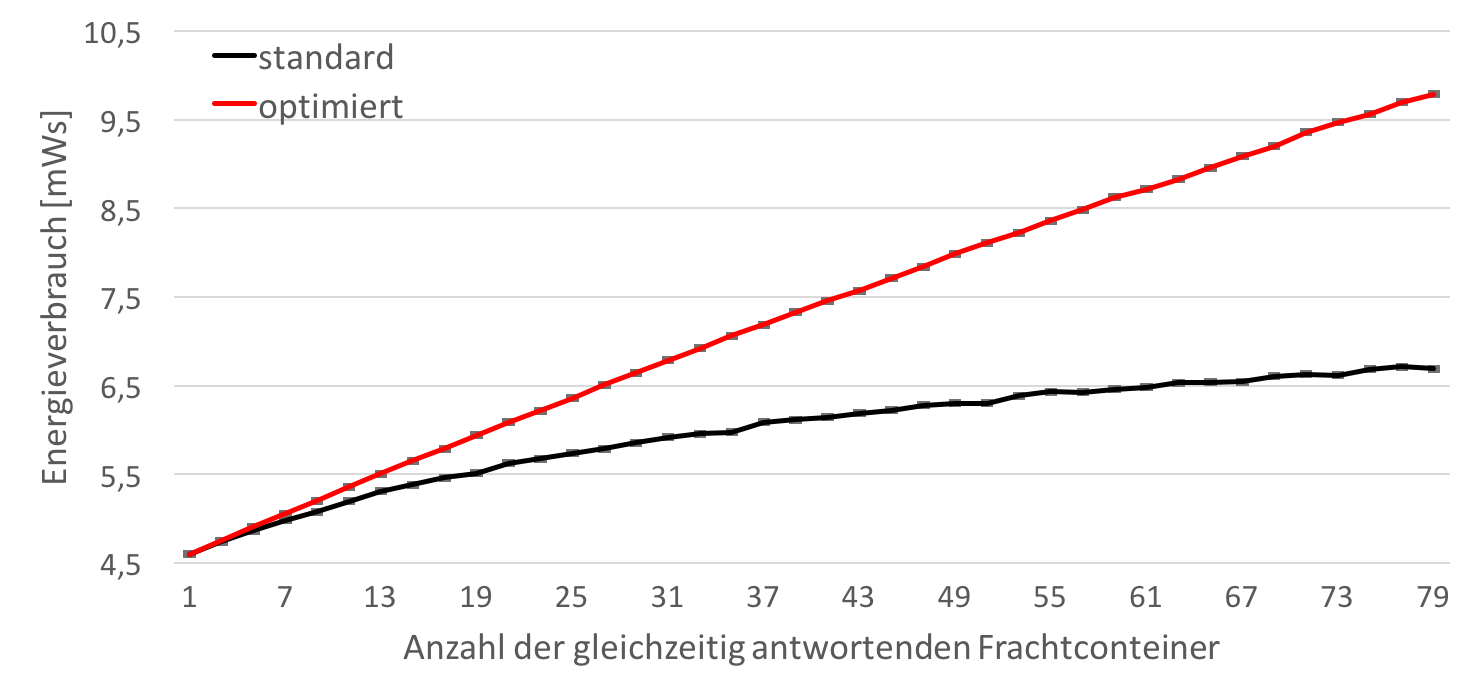
\includegraphics[width=1\linewidth]{gfx/Diag_Energie_1_80}} 
        \caption[Energieverbrauch]{ToDo}\label{fig:diag_Energie_1_80}
\end{figure}

Hinweis auf Energieverbrauch pro Sender während gesamter Laufzeit \\
Bezug von Energieverbruach auf erfolgreich zugestellte Nachrichten\\
--> dazu evtl. noch ein Diagramm \\
Energieverbrauch pro Sendeversuch \\

\begin{figure}[bth]
        \myfloatalign
        \subfloat[standard]
         {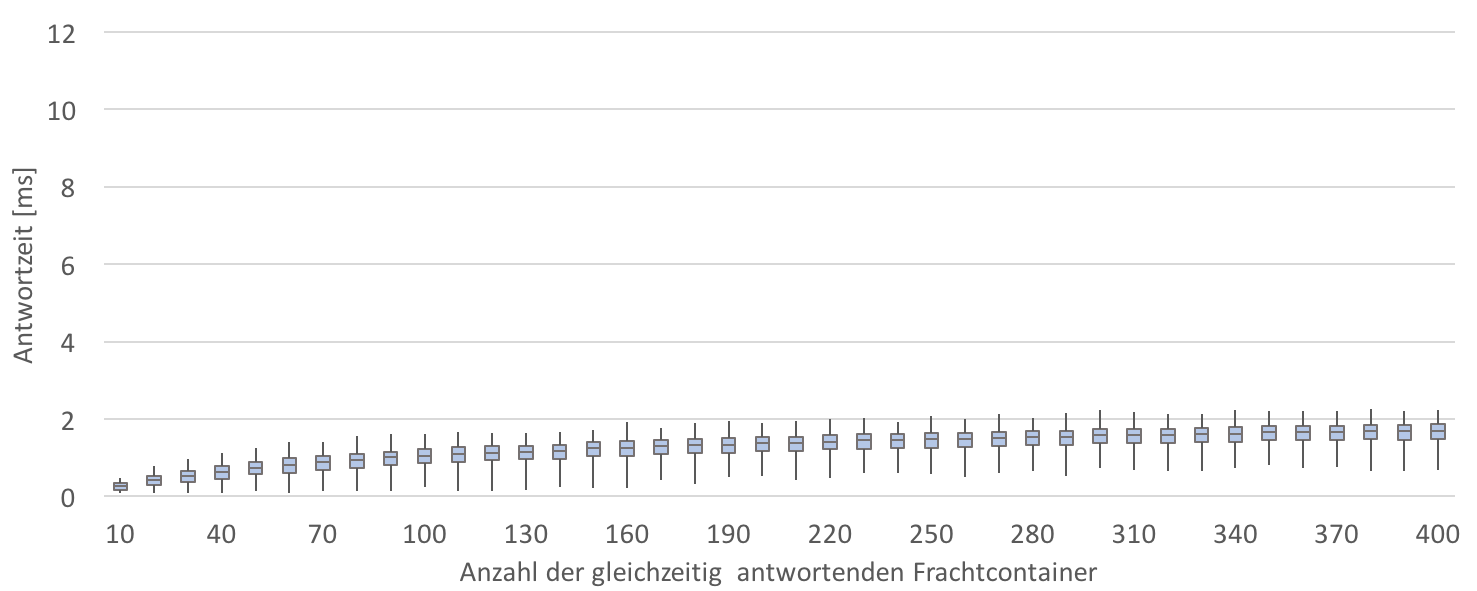
\includegraphics[width=1\linewidth]{gfx/Diag_Delay_std}} \\
        \subfloat[optimiert]
        {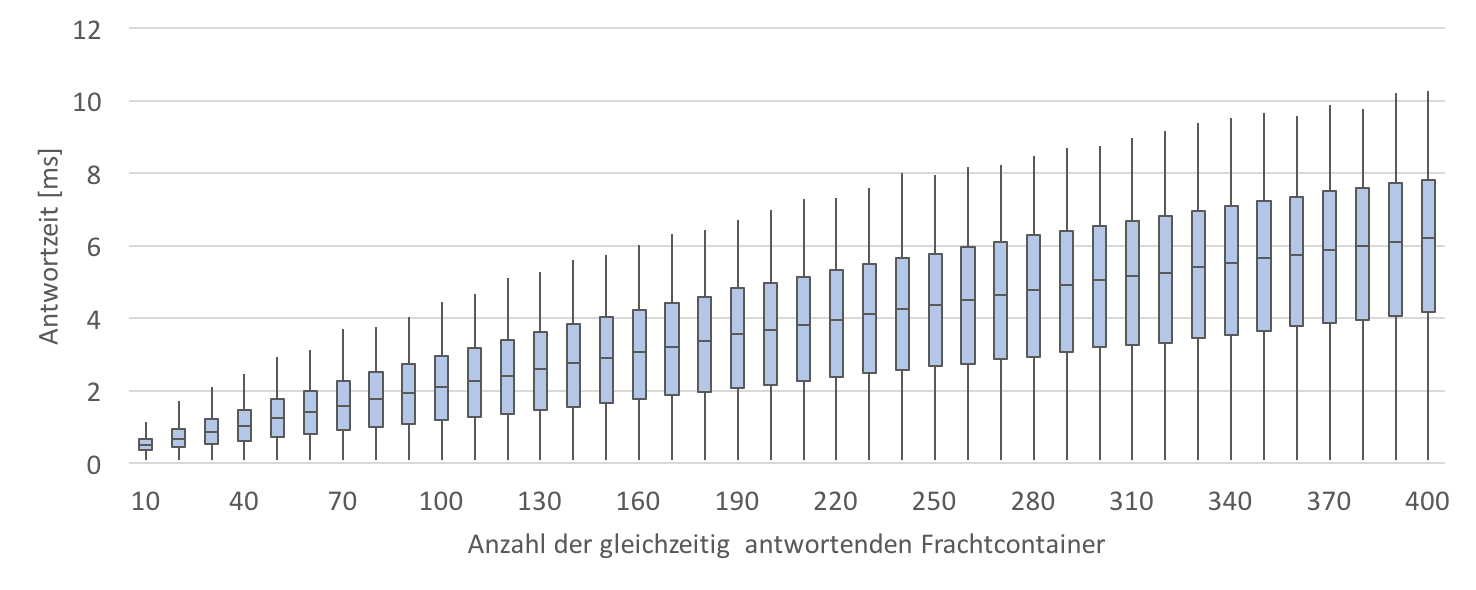
\includegraphics[width=1\linewidth]{gfx/Diag_Delay_opt}} 
        \caption[Verzögerung]{Boxplots der Antwortverzögerungen durch den \gls{csma} Algorithmus}\label{fig:diag_delay_1_400}
\end{figure}

Auswirkung der Algorithmus auf Antwortzeiten \\
Bezug und Bewertung dieses Effekts für das gegebene Szenario\\
Angabe von theoretischer oberer Schrake !? \\
Hinweis auf geringe Anzahl der Antworten insgesamt bei standard, wegen massiver Kollisionen
Hinweis zur Verteilung der einzelnen Antworten beim optimierten Verfahren\\
--> immer auch Anworten direkt nach Anfrage (Ausreißer nahe 0) --> effektive Kanalnutzung \\
dazu evtl noch Histogramm




%*****************************************
%*****************************************
%*****************************************
%*****************************************
%*****************************************





%************************************************
\chapter{Auswertung}\label{kap:auswertung}
%************************************************



%*****************************************
%*****************************************
%*****************************************
%*****************************************
%*****************************************





%************************************************
\chapter{Prototypische Implementierung}\label{kap:prototyp}
%************************************************

Beschreibung der Architektur \\

\section{Funktioinstest}

\begin{figure}[bth]
        \myfloatalign
        {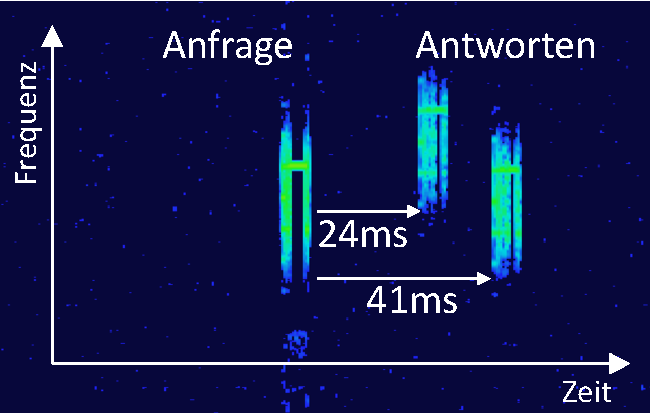
\includegraphics[width=0.6\linewidth]{gfx/Vers_01_Spac}} 
        \caption[Spektrumanalyzer]{ToDo}\label{fig:spac_2antworten}
\end{figure}

\begin{figure}[bth]
        \myfloatalign
        \subfloat[Terminal: Daten zur Übermittlung durch den \acs{ap}]
        {\label{fig:terminal-TX}%
         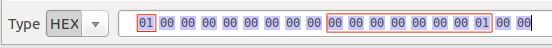
\includegraphics[width=0.8\linewidth]{gfx/ScS_Terminal_Send_markiert}} \\
        \subfloat[Terminal: Empfangene Daten am \acs{ap}]
        {\label{fig:terminal-RX}%
        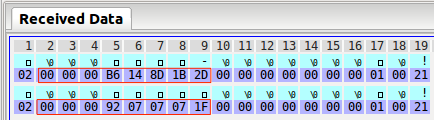
\includegraphics[width=0.8\linewidth]{gfx/ScS_Terminal_Rec_1x2Boxen_Vers_001_markiert}} 
        \caption[Terminal TX RX]{Ausschnitt aus dem Terminalprogramm \emph{hterm}. a) Sendezeile mit Bytes einer PAGE-Nachricht b) Empfagsbereich mit zwei QUANTITY-Nachrichten}\label{fig:terminal}
\end{figure}

\begin{figure}[bth]
        \myfloatalign
        {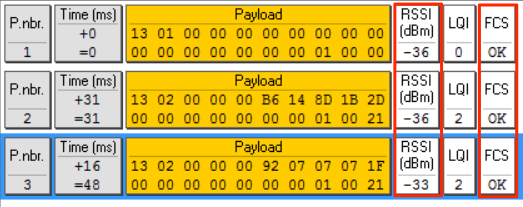
\includegraphics[width=0.8\linewidth]{gfx/ScS_Sniffer_AP_2Boxen_Vers_001_markiert}} 
        \caption[Sniffer]{Ausgabe der mitgeschnittenen Kommunikation in der \emph{Packet Sniffer} Software. Die Zusatzinforamtionen zu Signalstärke und Bitfehlern sind rot markiert.}\label{fig:sniffer}
\end{figure}

\begin{figure}[bth]
        \myfloatalign
        {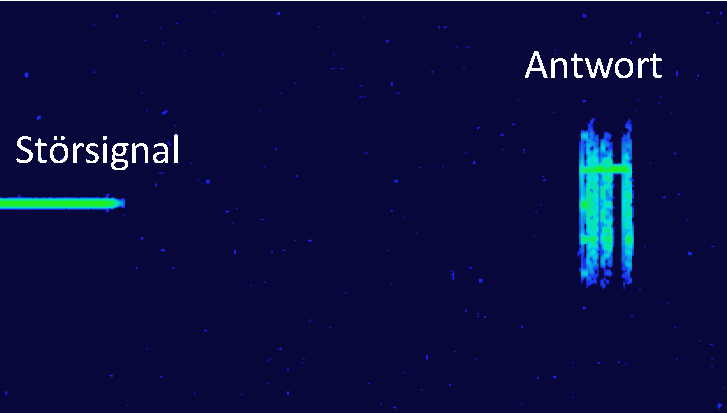
\includegraphics[width=0.6\linewidth]{gfx/Stoerer_Spac}} 
        \caption[Störsender]{Zeitlicher Verlauf der Kanalaktivität mit schmalbandigem Störsignal. Nachdem der Kanal frei ist, erscheint das Paket.}\label{fig:spac_stoerer}
\end{figure}

\section{Messungen}

\begin{figure}[bth]
        \myfloatalign
        \subfloat[Detaillierte Darstellung der Leistungsaufnahme über die Zeit bei $25ms$ Backoff]
        {\label{fig:power_csma_25zoom}%
         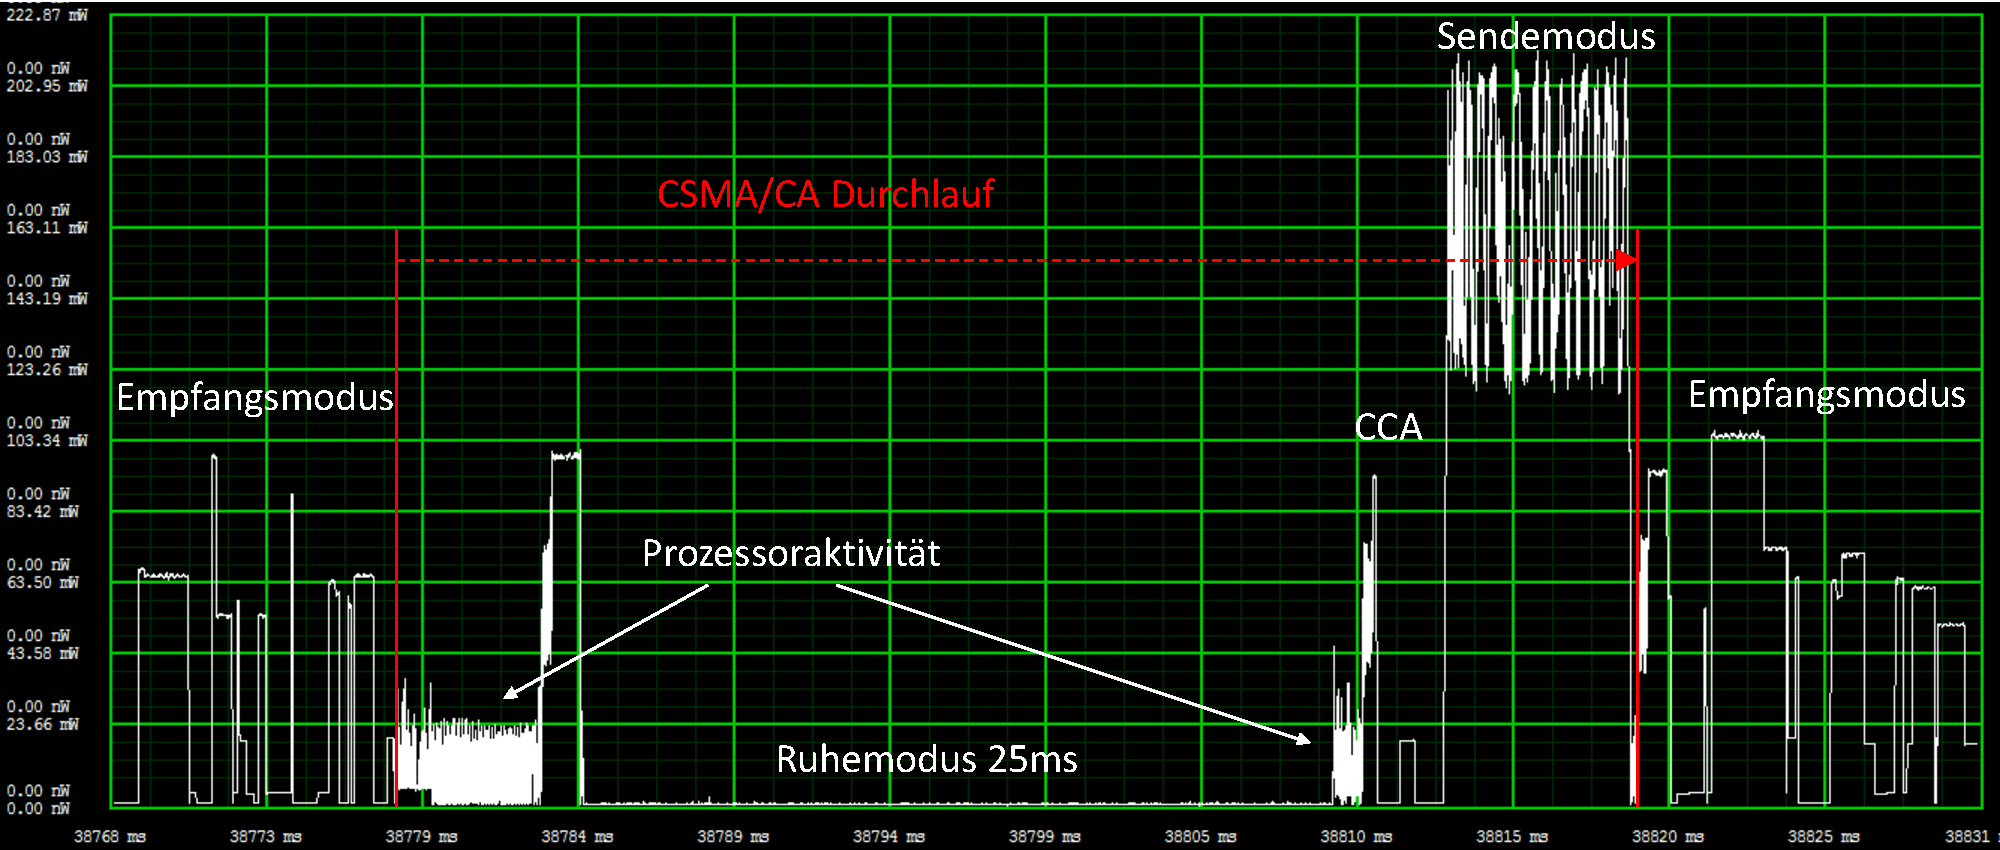
\includegraphics[width=1\linewidth]{gfx/Uebersicht_25_zoom_BO}} \\
        \subfloat[Leistungsaufnahme über die Zeit bei $34ms$ Backoff]
        {\label{fig:power_csma_34}%
        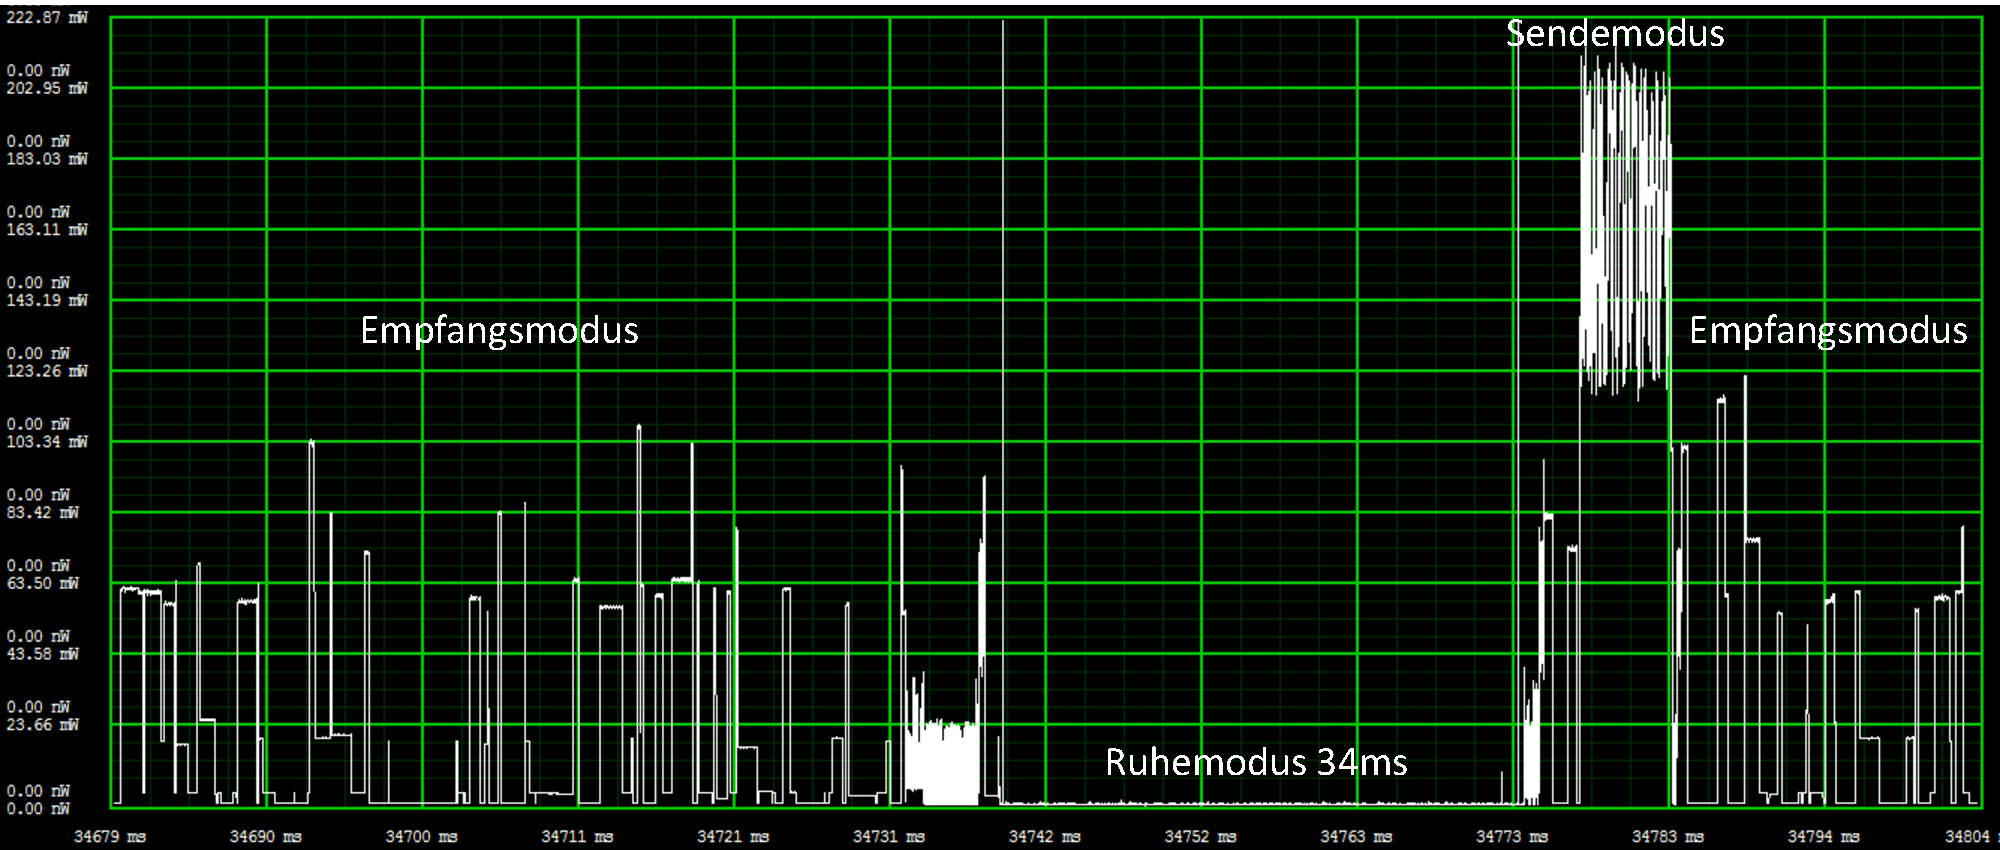
\includegraphics[width=1\linewidth]{gfx/Uebersicht_34_BO}} \\
        \subfloat[Leistungsaufnahme über die Zeit bei $101ms$ Backoff]
        {\label{fig:fig:power_csma_101}%
        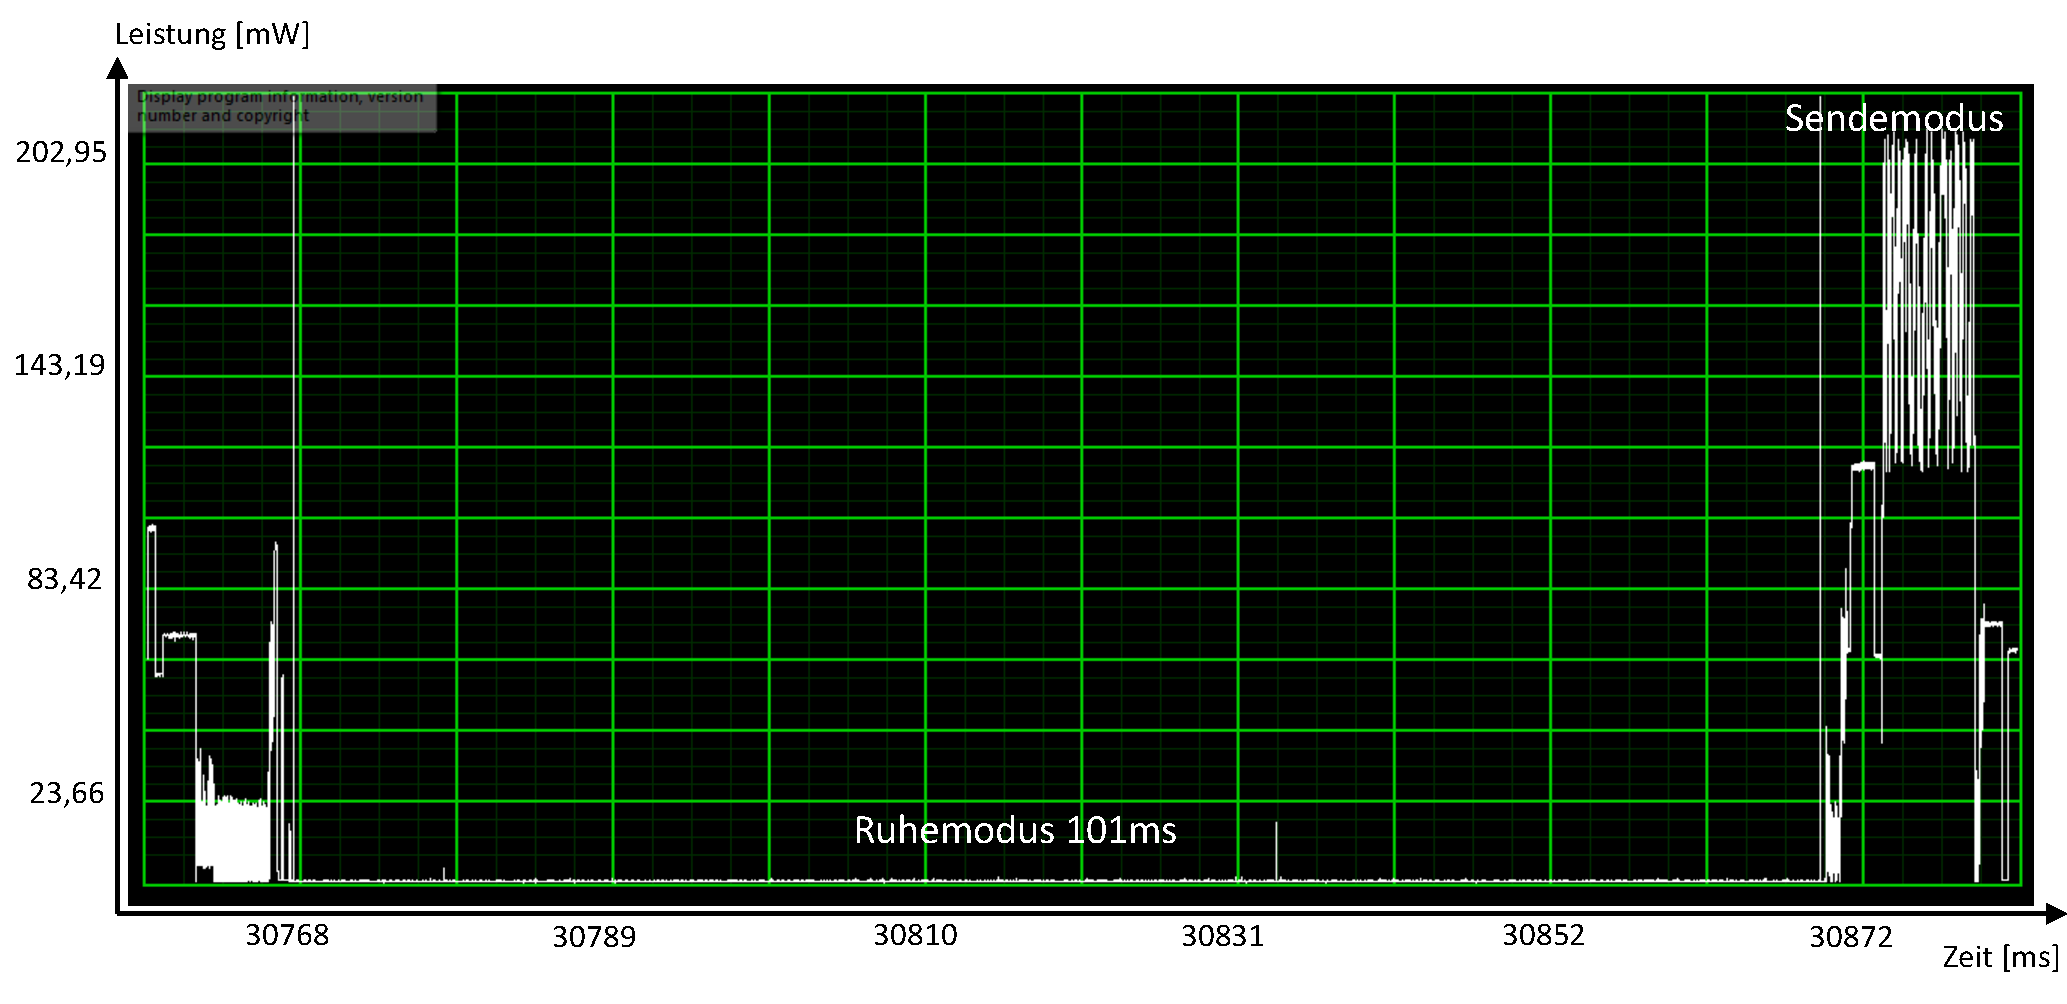
\includegraphics[width=1\linewidth]{gfx/Uebersicht_101_BO}} 
        \caption[Energiemessung CSMA/CA]{Drei Messungen des \emph{PowerScale} Systems zum Energieverbauch des cc1200 Funkchips während des \acs{csma} Algorithmus}\label{fig:power_csma}
\end{figure}

\begin{figure}[bth]
        \myfloatalign
        {\includegraphics[width=1\linewidth]{gfx/CCA_Stoerer_Power}} 
        \caption[Energiemessung CCA]{Analyse des Energieverbrauchs während des \acs{cca}. Da der Kanal durch ein Störsignalbelegt ist, werden währende des \acs{csma} Algorithmus wiederholt \acsp{cca} durchgeführt.}\label{fig:power_cca}
\end{figure}

\begin{figure}[bth]
        \myfloatalign
        \subfloat[]
        {\label{fig:diag_cca_dauer_leistung}%
         \includegraphics[width=0.75\linewidth]{gfx/Diag_CCA_Leistung_Dauer}} 
        \subfloat[]
        {\label{fig:diag_cca_energie}%
        \includegraphics[width=0.25\linewidth]{gfx/Diag_CCA_Boxplot_Energie}} 
        \caption[Energiemessung CCA]{Analyse des Energieverbrauchs: a) Punktdiagramm von 40 \acs{cca} Messungen. Ein Messpaar besteht aus der Dauer und der mittleren Leistungsaufnahme b) Boxplot zum resultierenden Energieverbrauch von 40 \acsp{cca}}\label{fig:diag_cca_dauer_leistung}
\end{figure}

\begin{figure}[bth]
        \myfloatalign
        {\includegraphics[width=0.6\linewidth]{gfx/Problem_Verarbeitung}} 
        \caption[Pakete mit kurzen Abstand]{Am \emph{Spectrum Analyzer} sind sieben Pakete zu sehen. Der Zwischenankunftszeit der letzten beiden Pakete liegt unter einer Millisekunde.}\label{fig:spec_pakete_mit_kurzem_abstand}
\end{figure}

%*****************************************
%*****************************************
%*****************************************
%*****************************************
%*****************************************





%************************************************
\chapter{Zusammenfassung}\label{kap:zusammenfassung}
%************************************************



%*****************************************
%*****************************************
%*****************************************
%*****************************************
%*****************************************





%\include{Chapters/VORLAGEN}
 

% ********************************************************************
% Backmatter
%*******************************************************
\appendix
%\renewcommand{\thechapter}{\alph{chapter}}
\cleardoublepage
%\part{Appendix}
%********************************************************************
% Appendix
%*******************************************************
% If problems with the headers: get headings in appendix etc. right
%\markboth{\spacedlowsmallcaps{Appendix}}{\spacedlowsmallcaps{Appendix}}
\chapter{CSMA/CA Blockdiagramm}\label{ahg:csmablock}
\begin{figure}[bth]
        \myfloatalign
        {\includegraphics[height=0.7\textheight]{gfx/CSMA-Block}} 
        \caption[CSMA/CA Blockdiagramm]{Blockdiagramm des \acs{csma} Algorithmus nach dem \acs{802154} Standard \citep{ieee}. }\label{fig:csma-block}
\end{figure}
%%********************************************************************
% Appendix
%*******************************************************
% If problems with the headers: get headings in appendix etc. right
%\markboth{\spacedlowsmallcaps{Appendix}}{\spacedlowsmallcaps{Appendix}}
\chapter{Energieverbrauch CSMA/CA }\label{ahg:messwerte_csma}
\begin{table}
    %\myfloatalign
  %\begin{tabularx}{1\textwidth}{Xll} \toprule
    \tableheadline{Messung} & \tableheadline{Energie \textrm{mWs}, 1 Sender} & \tableheadline{E in mWs, 10 Sender } \\ \midrule
    $1$  & $122mWh$ & $127mWh$ \\
    $2$  & $124mWh$ & $122mWh$ \\
    $3$ & $122mWh$ & $122mWh$ \\
    $4$  & $125mWh$ & $128mWh$ \\
    $5$  & $119mWh$ & $119mWh$ \\
    $6$  & $124mWh$ & $119mWh$ \\
    $7$  & $122mWh$ & $127mWh$ \\
    $8$  & $122mWh$ & $123mWh$ \\
    $9$  & $120mWh$ & $129mWh$ \\
    $10$  & $127mWh$ & $122mWh$ \\
    $11$  & $119mWh$ & $121mWh$ \\
    $12$  & $126mWh$ & $122mWh$ \\
    $13$  & $120mWh$ & $125mWh$ \\
    $14$  & $121mWh$ & $119mWh$ \\
    $15$  & $120mWh$ & $120mWh$ \\
    $16$  & $122mWh$ & $119mWh$ \\
    $17$  & $122mWh$ & $122mWh$ \\
    $18$  & $125mWh$ & $119mWh$ \\
    $19$  & $120mWh$ & $122mWh$ \\
    $20$  & $123mWh$ & $121mWh$ \\
    $21$  & $120mWh$ & $119mWh$ \\
    $22$  & $122mWh$ & $126mWh$ \\
    $23$  & $122mWh$ & $123mWh$ \\
    $24$  & $125mWh$ & $122mWh$ \\
    $25$  & $121mWh$ & $121mWh$ \\
    $26$  & $120mWh$ & $122mWh$ \\
    $27$  & $122mWh$ & $122mWh$\\
    $28$  & $122mWh$ & $120mWh$ \\
    $29$  & $122mWh$ & $122mWh$ \\
    $30$  & $122mWh$ & $121mWh$ \\
    $1$  & $122mWh$ & $127mWh$ \\
    $2$  & $124mWh$ & $122mWh$ \\
    $3$ & $122mWh$ & $122mWh$ \\
    $4$  & $125mWh$ & $128mWh$ \\
    $5$  & $119mWh$ & $119mWh$ \\
    $6$  & $124mWh$ & $119mWh$ \\
    $7$  & $122mWh$ & $127mWh$ \\
    $8$  & $122mWh$ & $123mWh$ \\
    $9$  & $120mWh$ & $129mWh$ \\
    $10$  & $127mWh$ & $122mWh$ \\
    $11$  & $119mWh$ & $121mWh$ \\
    $12$  & $126mWh$ & $122mWh$ \\
    $13$  & $120mWh$ & $125mWh$ \\
    $14$  & $121mWh$ & $119mWh$ \\
    $15$  & $120mWh$ & $120mWh$ \\
    $16$  & $122mWh$ & $119mWh$ \\
    $17$  & $122mWh$ & $122mWh$ \\
    $18$  & $125mWh$ & $119mWh$ \\
    $19$  & $120mWh$ & $122mWh$ \\
    $20$  & $123mWh$ & $121mWh$ \\
    $21$  & $120mWh$ & $119mWh$ \\
    $22$  & $122mWh$ & $126mWh$ \\
    $23$  & $122mWh$ & $123mWh$ \\
    $24$  & $125mWh$ & $122mWh$ \\
    $25$  & $121mWh$ & $121mWh$ \\
    $26$  & $120mWh$ & $122mWh$ \\
    $27$  & $122mWh$ & $122mWh$\\
    $28$  & $122mWh$ & $120mWh$ \\
    $29$  & $122mWh$ & $122mWh$ \\
    $30$  & $122mWh$ & $121mWh$ \\
    \midrule
    $\overline{x}$  & 122,1 & 122,2 \\
    \bottomrule
  %\end{tabularx}
  \caption[Messreihe EnergieVerbrauch]{Messreihen zum Energieverbrauch des \acs{csma} Algoithmus}  \label{tab:messreihe_csma_energie}
\end{table}

%********************************************************************
% Appendix
%*******************************************************
% If problems with the headers: get headings in appendix etc. right
%\markboth{\spacedlowsmallcaps{Appendix}}{\spacedlowsmallcaps{Appendix}}
\chapter{CC1200 Registerkonfiguration}\label{ahg:cc1200register}
\begin{lstlisting}[language=C,frame=b,captionpos=b,caption={Struktur mit Adresse-Wert Paaren für die Registerkonfiguration des CC1200 Funkchips},label=lst:cc1200register]
/*---------------------------------------------------
| File: fr_reg_config.h
|
| Save register configuration for CC1200 in rf_settings_t array.
| Defines register contents for CC1200 Register Space and
| Extended Register Space
|
| Created with TI Smart RF Studio 7
|
| Note: Uses #defines from rf.h
 --------------------------------------------------*/

#ifndef RF_REG_CONFIG_H
#define RF_REG_CONFIG_H

#include "rf.h"

static const rf_setting_t preferredSettings[]=
{
  {RF_IOCFG3,              0x06},
  {RF_IOCFG2,              0x0F}, /* TXONCCA_DONE*/
  {RF_IOCFG1,              0x30},
  {RF_IOCFG0,              0x06}, /* PKT_SYNC_RXTX*/
  {RF_SYNC3,               0x93},
  {RF_SYNC2,               0x0B},
  {RF_SYNC1,               0x51},
  {RF_SYNC0,               0xDE},
  {RF_SYNC_CFG1,           0xA9},
  {RF_SYNC_CFG0,           0x03},
  {RF_DEVIATION_M,         0x06},
  {RF_MODCFG_DEV_E,        0x0B},
  {RF_DCFILT_CFG,          0x4C},
  {RF_PREAMBLE_CFG1,       0x14},
  {RF_PREAMBLE_CFG0,       0x8A},
  {RF_IQIC,                0xC8},
  {RF_CHAN_BW,             0x10},
  {RF_MDMCFG1,             0x42},
  {RF_MDMCFG0,             0x05},
  {RF_SYMBOL_RATE2,        0x8F},
  {RF_SYMBOL_RATE1,        0x75},
  {RF_SYMBOL_RATE0,        0x10},
  {RF_AGC_REF,             0x27},
  {RF_AGC_CS_THR,          0x11}, /* -82dBm, add 99 due tue RSSI offset -> 17 -> 0x11*/
  {RF_AGC_GAIN_ADJUST,     0x00}, /* no RSSI offset stored, RSSI value will be 99dBm over reality, add -99 manually*/
  {RF_AGC_CFG3,            0xB1},
  {RF_AGC_CFG2,            0x20},
  {RF_AGC_CFG1,            0x11},
  {RF_AGC_CFG0,            0x9C}, /* 0x94 -> 0x9C RSSI_VALID_CNT = 9*/
  {RF_FIFO_CFG,            0x00},
  {RF_DEV_ADDR,            0x00},
  {RF_SETTLING_CFG,        0x0B},
  {RF_FS_CFG,              0x12},
  {RF_WOR_CFG1,            0x08},
  {RF_WOR_CFG0,            0x21},
  {RF_WOR_EVENT0_MSB,      0x00},
  {RF_WOR_EVENT0_LSB,      0x00},
  {RF_RXDCM_TIME,          0x00},
  {RF_PKT_CFG2,            0x04}, /* CCA_MODE = 001 (RSSI below threshold)*/
  {RF_PKT_CFG1,            0x03},
  {RF_PKT_CFG0,            0x20},
  {RF_RFEND_CFG1,          0x0F},
  {RF_RFEND_CFG0,          0x00},
  {RF_PA_CFG1,             0x7F},
  {RF_PA_CFG0,             0x56},
  {RF_ASK_CFG,             0x0F},
  {RF_PKT_LEN,             0xFF},
  {RF_IF_MIX_CFG,          0x1C},
  {RF_FREQOFF_CFG,         0x20},
  {RF_TOC_CFG,             0x03},
  {RF_MARC_SPARE,          0x00},
  {RF_ECG_CFG,             0x00},
  {RF_MDMCFG2,             0x02},
  {RF_EXT_CTRL,            0x01},
  {RF_RCCAL_FINE,          0x00},
  {RF_RCCAL_COARSE,        0x00},
  {RF_RCCAL_OFFSET,        0x00},
  {RF_FREQOFF1,            0x00},
  {RF_FREQOFF0,            0x00},
  {RF_FREQ2,               0x56},
  {RF_FREQ1,               0xCC},
  {RF_FREQ0,               0xCC},
  {RF_IF_ADC2,             0x02},
  {RF_IF_ADC1,             0xEE},
  {RF_IF_ADC0,             0x10},
  {RF_FS_DIG1,             0x07},
  {RF_FS_DIG0,             0xAF},
  {RF_FS_CAL3,             0x00},
  {RF_FS_CAL2,             0x20},
  {RF_FS_CAL1,             0x40},
  {RF_FS_CAL0,             0x0E},
  {RF_FS_CHP,              0x28},
  {RF_FS_DIVTWO,           0x03},
  {RF_FS_DSM1,             0x00},
  {RF_FS_DSM0,             0x33},
  {RF_FS_DVC1,             0xFF},
  {RF_FS_DVC0,             0x17},
  {RF_FS_LBI,              0x00},
  {RF_FS_PFD,              0x00},
  {RF_FS_PRE,              0x6E},
  {RF_FS_REG_DIV_CML,      0x1C},
  {RF_FS_SPARE,            0xAC},
  {RF_FS_VCO4,             0x14},
  {RF_FS_VCO3,             0x00},
  {RF_FS_VCO2,             0x00},
  {RF_FS_VCO1,             0x00},
  {RF_FS_VCO0,             0xB5},
  {RF_GBIAS6,              0x00},
  {RF_GBIAS5,              0x02},
  {RF_GBIAS4,              0x00},
  {RF_GBIAS3,              0x00},
  {RF_GBIAS2,              0x10},
  {RF_GBIAS1,              0x00},
  {RF_GBIAS0,              0x00},
  {RF_IFAMP,               0x09},
  {RF_LNA,                 0x01},
  {RF_RXMIX,               0x01},
  {RF_XOSC5,               0x0E},
  {RF_XOSC4,               0xA0},
  {RF_XOSC3,               0x03},
  {RF_XOSC2,               0x04},
  {RF_XOSC1,               0x03},
  {RF_XOSC0,               0x00},
  {RF_ANALOG_SPARE,        0x00},
  {RF_PA_CFG3,             0x00},
  {RF_WOR_TIME1,           0x00},
  {RF_WOR_TIME0,           0x00},
  {RF_WOR_CAPTURE1,        0x00},
  {RF_WOR_CAPTURE0,        0x00},
  {RF_BIST,                0x00},
  {RF_DCFILTOFFSET_I1,     0x00},
  {RF_DCFILTOFFSET_I0,     0x00},
  {RF_DCFILTOFFSET_Q1,     0x00},
  {RF_DCFILTOFFSET_Q0,     0x00},
  {RF_IQIE_I1,             0x00},
  {RF_IQIE_I0,             0x00},
  {RF_IQIE_Q1,             0x00},
  {RF_IQIE_Q0,             0x00},
  {RF_RSSI1,               0x80},
  {RF_RSSI0,               0x00},
  {RF_MARCSTATE,           0x41},
  {RF_LQI_VAL,             0x00},
  {RF_PQT_SYNC_ERR,        0xFF},
  {RF_DEM_STATUS,          0x00},
  {RF_FREQOFF_EST1,        0x00},
  {RF_FREQOFF_EST0,        0x00},
  {RF_AGC_GAIN3,           0x00},
  {RF_AGC_GAIN2,           0xD1},
  {RF_AGC_GAIN1,           0x00},
  {RF_AGC_GAIN0,           0x3F},
  {RF_CFM_RX_DATA_OUT,     0x00},
  {RF_CFM_TX_DATA_IN,      0x00},
  {RF_ASK_SOFT_RX_DATA,    0x30},
  {RF_RNDGEN,              0xFF}, // enable Rnd Num Gen NO RETENTION when going to sleep !!!
  {RF_MAGN2,               0x00},
  {RF_MAGN1,               0x00},
  {RF_MAGN0,               0x00},
  {RF_ANG1,                0x00},
  {RF_ANG0,                0x00},
  {RF_CHFILT_I2,           0x02},
  {RF_CHFILT_I1,           0x00},
  {RF_CHFILT_I0,           0x00},
  {RF_CHFILT_Q2,           0x00},
  {RF_CHFILT_Q1,           0x00},
  {RF_CHFILT_Q0,           0x00},
  {RF_GPIO_STATUS,         0x00},
  {RF_FSCAL_CTRL,          0x01},
  {RF_PHASE_ADJUST,        0x00},
  {RF_PARTNUMBER,          0x20},
  {RF_PARTVERSION,         0x11},
  {RF_SERIAL_STATUS,       0x00},
  {RF_MODEM_STATUS1,       0x10},
  {RF_MODEM_STATUS0,       0x00},
  {RF_MARC_STATUS1,        0x00},
  {RF_MARC_STATUS0,        0x00},
  {RF_PA_IFAMP_TEST,       0x00},
  {RF_FSRF_TEST,           0x00},
  {RF_PRE_TEST,            0x00},
  {RF_PRE_OVR,             0x00},
  {RF_ADC_TEST,            0x00},
  {RF_DVC_TEST,            0x0B},
  {RF_ATEST,               0x40},
  {RF_ATEST_LVDS,          0x00},
  {RF_ATEST_MODE,          0x00},
  {RF_XOSC_TEST1,          0x3C},
  {RF_XOSC_TEST0,          0x00},
  {RF_AES,                 0x00},
  {RF_MDM_TEST,            0x00},
  {RF_RXFIRST,             0x00},
  {RF_TXFIRST,             0x00},
  {RF_RXLAST,              0x00},
  {RF_TXLAST,              0x00},
  {RF_NUM_TXBYTES,         0x00},
  {RF_NUM_RXBYTES,         0x00},
  {RF_FIFO_NUM_TXBYTES,    0x0F},
  {RF_FIFO_NUM_RXBYTES,    0x00},
  {RF_RXFIFO_PRE_BUF,      0x00},
  {RF_AES_KEY15,           0x00},
  {RF_AES_KEY14,           0x00},
  {RF_AES_KEY13,           0x00},
  {RF_AES_KEY12,           0x00},
  {RF_AES_KEY11,           0x00},
  {RF_AES_KEY10,           0x00},
  {RF_AES_KEY9,            0x00},
  {RF_AES_KEY8,            0x00},
  {RF_AES_KEY7,            0x00},
  {RF_AES_KEY6,            0x00},
  {RF_AES_KEY5,            0x00},
  {RF_AES_KEY4,            0x00},
  {RF_AES_KEY3,            0x00},
  {RF_AES_KEY2,            0x00},
  {RF_AES_KEY1,            0x00},
  {RF_AES_KEY0,            0x00},
  {RF_AES_BUFFER15,        0x00},
  {RF_AES_BUFFER14,        0x00},
  {RF_AES_BUFFER13,        0x00},
  {RF_AES_BUFFER12,        0x00},
  {RF_AES_BUFFER11,        0x00},
  {RF_AES_BUFFER10,        0x00},
  {RF_AES_BUFFER9,         0x00},
  {RF_AES_BUFFER8,         0x00},
  {RF_AES_BUFFER7,         0x00},
  {RF_AES_BUFFER6,         0x00},
  {RF_AES_BUFFER5,         0x00},
  {RF_AES_BUFFER4,         0x00},
  {RF_AES_BUFFER3,         0x00},
  {RF_AES_BUFFER2,         0x00},
  {RF_AES_BUFFER1,         0x00},
  {RF_AES_BUFFER0,         0x00},
};

#endif
\end{lstlisting}

%********************************************************************
% Appendix
%*******************************************************
% If problems with the headers: get headings in appendix etc. right
%\markboth{\spacedlowsmallcaps{Appendix}}{\spacedlowsmallcaps{Appendix}}
\chapter{CSMA/CA Implementierung}\label{ahg:implementierung}

\begin{lstlisting}[language=C,frame=b,captionpos=b,caption={Auszug aus dem Quellcode des Prototypen: Implementierung der Sendefunktion.},label=lst:implementierung_send]
/////////////////////////////////////

//!  PUBLIC rf_send()
//!
/////////////////////////////////////
void rf_send_fix(com_frame_t* frame) {

	uint8  status = 0;
	uint8  cca_state;
	uint16 tx_on_cca_failed;
	uint8  writeByte;
	uint8  rnd;
	uint16 backoff;

	// Configure GPIO Interrupt
    // no ISR no INT enable just set the right edge select
    // for chekcing the ISR flag on P3.4 later for end of transmission.
    // Line connected to P3.4 looks like this:
    //
    //          start sending               send complete
    //               ___________________________
    // _____________|                           |_____
    //
    P3DIR &= ~BIT4;                 // Set P3.4 to input direction
    P3REN |= BIT4;                  // Set P3.4 pullup/down Resistor
    P3OUT &= ~BIT4;                 // Select P3.4 pull-down
    P3IE  &= ~BIT4;                 // Disable Interrupt on P3.4
    P3IES |= BIT4;                  // falling edge
    P3IFG &= ~BIT4;                 // clear P3.4 interrupt flag

	// copy data frame into txBuffer
	// add length byte
	txBuffer[0] = RF_PAYLOADLEN;
	uint16 i;
	for(i=0; i<RF_PAYLOADLEN; i++){
		txBuffer[i+1] = frame->array[(RF_PAYLOADLEN)-1-i];
	}


	// enter CSMA
	while(csma_state == BUSY){

	    // choose random backoff
	    status = spi_cmd_strobe(RF_SRX); // RX state for further randomized number
	    status = read_reg(RF_RNDGEN, &rnd, 1);
	    backoff = (uint16) (rnd & 0b0000000001111111); // use all 7 Bits -> 0 to 127
	    status = read_reg(RF_RNDGEN, &rnd, 1);
        backoff += (uint16) (rnd & 0b0000000001111111); // use all 7 Bits again -> 0 to 255

	    // put CC1200 into SLEEP during backoff
	    status = spi_cmd_strobe(RF_SIDLE);
	    status = spi_cmd_strobe(RF_SPWD);  // until CS goes LOW again

        // backoff (blocking)
        TA3CCR0 = 0;                       // stop timer
        TA3CTL |= TACLR;                   // clear count value
        TA3CCTL0 &= ~CCIFG;                // clear TACCR3 interrupt flag
        TA3CCR0 = 125;                     // start timer SMCLK/8/125 = 1kHz => 1ms
        while(backoff != 0){               // wait for backoff counter
            while(!(TA3CCTL0 & CCIFG));    // wait for interrupt flag -> (ISR disabled)
            TA3CCTL0 &= ~CCIFG;            // clear TACCR3 interrupt flag
            backoff --;
        }

        //Wake Up
        status = spi_cmd_strobe(RF_SIDLE); // wake up CC1200
        status = spi_cmd_strobe(RF_SNOP);  // debugging
        writeByte = 0xFF;
        status = write_reg(RF_RNDGEN, &writeByte, 1); // reactivate RNDGEN, no retention reg!


        // ensure RX mode and CARRIER_SENSE_VALID
        writeByte = 0x10;                  // 16->CARRIER_SENSE_VALID
        status = write_reg(RF_IOCFG2, &writeByte, 1);
        P3IFG &= ~BIT5;                    // clear P3.5 interrupt flag
        status = spi_cmd_strobe(RF_SRX);   // ensure RX to perform CCA
        status = spi_cmd_strobe(RF_SNOP);  // debugging
        while(!(P3IFG & BIT5));            // wait for CS to be valid -> interrupt an P3.5 (ISR disabled)
        P3IFG &= ~BIT5;                    // clear P3.5 interrupt flag

        // Write packet to TX FIFO
        status = write_tx_fifo(txBuffer, sizeof(txBuffer));

        // try to send
        writeByte = 0x0F;                  // 15->TXONCCA_DONE
        status = write_reg(RF_IOCFG2, &writeByte, 1);
        P3IFG &= ~BIT5;                    // clear P3.5 interrupt flag
        status = spi_cmd_strobe(RF_STX);   // try to send
        while(!(P3IFG & BIT5));            // wait for CCA decision -> interrupt an P3.5 (ISR disabled)
        P3IFG &= ~BIT5;                    // clear P3.5 interrupt flag

        // debugging
        status = read_reg(RF_RSSI1, &rssi, 1);

        //check CCA state
        status = read_reg(RF_MARC_STATUS0, &cca_state, 1);
        tx_on_cca_failed = (cca_state & 0b00000100);
        if(!tx_on_cca_failed){ // NOT TXONCCA_FAILED
            csma_state = SUCCESS;
        }
	}
	csma_state = BUSY;

	// wait for interruptflag that packet has been sent.
	// assuming the CC1200-GPIO connected to P3.4 is
	// set to GPIOx_CFG = 0x06 -> CC1200 PKT_SYNC_RXTX interrupt
	while(!(P3IFG & BIT4));
	status = spi_cmd_strobe(RF_SNOP);

	//flush TX FIFO
	status = spi_cmd_strobe(RF_SIDLE);
	status = spi_cmd_strobe(RF_SFTX);

	status = spi_cmd_strobe(RF_SRX);
	P3IFG &= ~BIT4;                 // clear P3.4 interrupt flag
	P3IE  |= BIT4;                  // Enable Interrupt on P3.4
	P3IFG &= ~BIT4;                 // clear P3.4 interrupt flag
}


//###################################
// interrupt service routines:
//###################################

/////////////////////////////////////////////////////////////////

//!  PORT3.4 ISR indicating 'TX complete' as well as 'new data arrived'
//!
/////////////////////////////////////////////////////////////////

#pragma vector=PORT3_VECTOR
__interrupt void Port_3(void)
{
	P3IE &= ~BIT4;                              // Disable Interrupt on P3.4

	uint8 status;
	status = read_rx_fifo(rxBuffer, sizeof(rxBuffer));

	if (rxBuffer[21] & 0b10000000) {       // chech CRC
		g_callback((rxBuffer), SRC_RF);       // pointer of secound byte, skip length byte
	}
	// flush RX-FIFO
	status = spi_cmd_strobe(RF_SIDLE);
	status = spi_cmd_strobe(RF_SFRX);

	status = spi_cmd_strobe(RF_SRX);

	P3IE  |= BIT4;                                  // Enable Interrupt on P3.4
	P3IFG &= ~BIT4;                             // clear P3.4 interrupt flag
}
\end{lstlisting}
%********************************************************************
% Appendix
%*******************************************************
% If problems with the headers: get headings in appendix etc. right
%\markboth{\spacedlowsmallcaps{Appendix}}{\spacedlowsmallcaps{Appendix}}
\chapter{Zufallszahlenerzeugung}\label{ahg:rnd}

\begin{figure}[bth]
        \myfloatalign
        \subfloat[]
        {\label{fig:diag_scatter_pseudo}%
         \includegraphics[width=1\linewidth]{gfx/Diag_RNG_pseudo}} \\
        \subfloat[]
        {\label{fig:diag_scatter_real}%
        \includegraphics[width=1\linewidth]{gfx/Diag_RNG_Rauschen}} 
        \caption[Zufallszahlen]{Analyse der vom CC1200 Funkchip erzeugten Zufallszahlen. a) Vom Prozessor erzeugte Pseudozufallszahlen b) Pseuduzufallszahlen kombiniert mit Empfängerrauschen}\label{fig:diag_scatter_rng}
\end{figure}
%********************************************************************
% Other Stuff in the Back
%*******************************************************
\cleardoublepage%********************************************************************
% Bibliography
%*******************************************************
% work-around to have small caps also here in the headline
\manualmark
\markboth{\spacedlowsmallcaps{\bibname}}{\spacedlowsmallcaps{\bibname}} % work-around to have small caps also
%\phantomsection 
\refstepcounter{dummy}
\addtocontents{toc}{\protect\vspace{\beforebibskip}} % to have the bib a bit from the rest in the toc
\addcontentsline{toc}{chapter}{\tocEntry{\bibname}}
\label{app:bibliography}
\printbibliography

%\cleardoublepage%*******************************************************
% Declaration
%*******************************************************
\refstepcounter{dummy}
\pdfbookmark[0]{Declaration}{declaration}
\chapter*{Declaration}
\thispagestyle{empty}
Put your declaration here.
\bigskip
 
\noindent\textit{\myLocation, \myTime}

\smallskip

\begin{flushright}
    \begin{tabular}{m{5cm}}
        \\ \hline
        \centering\myName \\
    \end{tabular}
\end{flushright}

\cleardoublepage\makeatletter
\cleardoublepage
\thispagestyle{empty}
%\onehalfspacing
\linespread{1.25}
\LARGE
\begin{center}
	\textbf{Eidesstattliche Versicherung}
\end{center}

\small
\vspace{\baselineskip}
\underline{\makebox[.4\textwidth][c]{\mySurname, \myForename}}
\hspace{.25\textwidth}
\underline{\makebox[.3\textwidth][c]{\myMatNr}}
\newline
\makebox[.4\textwidth][l]{Name, Vorname}
\hspace{.25\textwidth}
\makebox[.3\textwidth][l]{Matr.-Nr.}
\vspace{\baselineskip}

\noindent Ich versichere hiermit an Eides statt, dass ich die vorliegende \myDocType\space mit dem Titel

%\begin{center}
%underline{\makebox[0.97\textwidth][c]{\textit{\myTitle}}}
%\end{center}

\begin{center}
\textit{\myTitle}
%\underline{\makebox[0.97\textwidth][c]{\textit{\myTitle}}}
\end{center}

\noindent selbstständig und ohne unzulässige fremde Hilfe erbracht habe. Ich habe keine anderen als die 
angegebenen Quellen und Hilfsmittel benutzt sowie wörtliche und sinngemäße Zitate kenntlich 
gemacht. Die Arbeit hat in gleicher oder ähnlicher Form noch keiner Prü\-fungs\-be\-hörde 
vorgelegen. 
\vspace{\baselineskip}

\underline{\makebox[.4\textwidth][c]{\myLocation, \myDate}} % FIXME: Ort und Datum evtl. weglassen und handschriftlich nach Druck einfügen
\hspace{.25\textwidth}
\underline{\hspace{.3\textwidth}}
\newline
\makebox[.4\textwidth][l]{Ort, Datum}
\hspace{.25\textwidth}
\makebox[.3\textwidth][l]{Unterschrift}

\vspace{\baselineskip}

\noindent \textbf{Belehrung}: 

\noindent Wer vorsätzlich gegen eine die Täuschung über Prüfungsleistungen betreffende Regelung einer 
Hochschulprüfungsordnung verstößt, handelt ordnungswidrig. Die Ordnungswidrigkeit kann mit 
einer Geldbuße von bis zu 50.000,00\,€ geahndet werden. Zuständige Verwaltungs\-behörde für 
die Verfolgung und Ahndung von Ordnungswidrigkeiten ist der Kanzler/die Kanzlerin der 
Technischen Universität Dortmund. Im Falle eines mehrfachen oder sonstigen schwerwiegenden 
Täuschungs\-versuches kann der Prüfling zudem exmatrikuliert werden. (§ 63 Abs. 5 
Hochschulgesetz - HG - )  

\noindent Die Abgabe einer falschen Versicherung an Eides statt wird mit Freiheitsstrafe bis zu 3 Jahren 
oder mit Geldstrafe bestraft.  

\noindent Die Technische Universität Dortmund wird ggf. elektronische Vergleichswerkzeuge (wie z.B. die 
Software „turnitin“) zur Überprüfung von Ordnungswidrigkeiten in Prüfungsverfahren nutzen. 

\noindent Die oben stehende Belehrung habe ich zur Kenntnis genommen: 
\vspace{\baselineskip}

\underline{\makebox[.4\textwidth][c]{\myLocation, \myDate}}
\hspace{.25\textwidth}
\underline{\hspace{.3\textwidth}}
\newline
\makebox[.4\textwidth][l]{Ort, Datum}
\hspace{.25\textwidth}
\makebox[.3\textwidth][l]{Unterschrift}
\makeatother
%\cleardoublepage\pagestyle{empty}

\hfill

\vfill


\pdfbookmark[0]{Colophon}{colophon}
\section*{Colophon}
This document was typeset using the typographical look-and-feel \texttt{classicthesis} developed by Andr\'e Miede. 
The style was inspired by Robert Bringhurst's seminal book on typography ``\emph{The Elements of Typographic Style}''. 
\texttt{classicthesis} is available for both \LaTeX\ and \mLyX: 
\begin{center}
\url{https://bitbucket.org/amiede/classicthesis/}
\end{center}
Happy users of \texttt{classicthesis} usually send a real postcard to the author, a collection of postcards received so far is featured here: 
\begin{center}
\url{http://postcards.miede.de/}
\end{center}
 
\bigskip

\noindent\finalVersionString

%Hermann Zapf's \emph{Palatino} and \emph{Euler} type faces (Type~1 PostScript fonts \emph{URW
%Palladio L} and \emph{FPL}) are used. The ``typewriter'' text is typeset in \emph{Bera Mono}, 
%originally developed by Bitstream, Inc. as ``Bitstream Vera''. (Type~1 PostScript fonts were made 
%available by Malte Rosenau and
%Ulrich Dirr.)

%\paragraph{note:} The custom size of the textblock was calculated
%using the directions given by Mr. Bringhurst (pages 26--29 and
%175/176). 10~pt Palatino needs  133.21~pt for the string
%``abcdefghijklmnopqrstuvwxyz''. This yields a good line length between
%24--26~pc (288--312~pt). Using a ``\emph{double square textblock}''
%with a 1:2 ratio this results in a textblock of 312:624~pt (which
%includes the headline in this design). A good alternative would be the
%``\emph{golden section textblock}'' with a ratio of 1:1.62, here
%312:505.44~pt. For comparison, \texttt{DIV9} of the \texttt{typearea}
%package results in a line length of 389~pt (32.4~pc), which is by far
%too long. However, this information will only be of interest for
%hardcore pseudo-typographers like me.%
%
%To make your own calculations, use the following commands and look up
%the corresponding lengths in the book:
%\begin{verbatim}
%    \settowidth{\abcd}{abcdefghijklmnopqrstuvwxyz}
%    \the\abcd\ % prints the value of the length
%\end{verbatim}
%Please see the file \texttt{classicthesis.sty} for some precalculated 
%values for Palatino and Minion.
%
%    \settowidth{\abcd}{abcdefghijklmnopqrstuvwxyz}
%    \the\abcd\ % prints the value of the length





% ********************************************************************
% Game Over: Restore, Restart, or Quit?
%*******************************************************
\end{document}
% ********************************************************************
